% !TEX encoding = UTF-8
% !TEX TS-program = pdflatex
% !TEX root = ../thesis.tex

%**************************************************************
\chapter{STATO DELL'ARTE}
\label{Capitolo2}
\thispagestyle{empty}

Il tema della guida autonoma si sta sempre più affermando come importante 
oggetto di studio nella comunità scientifica. Visto il grande impiego di sistemi 
basati sul Machine Learning, in particolare le reti neurali, in questa sezione 
verranno introdotti alcuni concetti atti a rappresentare sia la struttura di tali 
sistemi che la loro influenza nell'ambiente automotive. 

\section{Reti Neurali Biologiche}
Il cervello umano ha la capacità di sfruttare la sua struttura di neuroni in modo 
da eseguire più calcoli rispetto a un comune computer. Mediamente ogni cervello 
contiene un numero di neuroni pari a $10^{11}$. La struttura di un neurone biologico 
è quello mostrata in figura (\ref{biological neuron}):
\begin{figure}
    \centering
    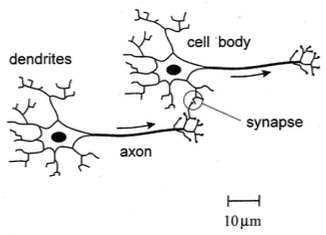
\includegraphics[width = 0.6 \linewidth]{images/biological neuron.png}
    \centering
    \caption{Composizione di due neuroni biologici.}
    \label{biological neuron}
\end{figure}
Da come possiamo notare, esistono vari componenti che costituiscono un 
neurone. In particolare, abbiamo i \emph{dendriti} che rappresentano gli ingressi di un 
neurone mentre le uscite sono rappresentare dagli \emph{assoni}. Su ogni assone viaggia 
un impulso elettrico generato dal neurone stesso quando questo si trova in uno 
stato attivo. Ogni neurone è connesso a migliaia di suoi simili ed ogni 
comunicazione fra questi avviene mediante le sinapsi. Quando l'impulso raggiunge 
proprio le sinapsi, questo provoca il rilascio di sostanze chimiche che attraversano 
la giunzioni ed entrano all'interno di altri neuroni. Ci sono due tipologie di sinapsi, 
eccitatori e inibitori. La prima tipologia permette di aumentare la probabilità che 
un neurone si attivi. Tale probabilità è determinata dal peso associato ad ogni 
sinapsi. Avendo multipli collegamenti, ogni neurone effettua una specie di somma 
pesata degli ingressi che, se maggiore di una determinata soglia, può provocare la 
sua attivazione. 

\section{Reti Neurali Artificiali}\label{Reti neurali}
Una rete neurale artificiale è un modello computazionale che, a partire da dei dati 
di input, riesce a produrre un output mediante un meccanismo ispirato a quello 
del cervello umano. Alla base di questa similitudine, tali reti prendono il nome di 
\emph{Artificial Neural Networks (ANN)}. Le prime reti neurali, nate attorno gli anni 
'50, basavano il loro funzionamento sui cosiddetti \emph{percettroni}, neuroni artificiali in 
grado di apprendere e di accumulare esperienza. Ogni rete neurale è composta da 
strati di neuroni, comunemente chiamati \emph{layers}. I dati di input saranno processati 
dai neuroni presenti nell'input layer e da qui, i risultati ottenuti, si propagheranno 
verso i layer nascosti (hidden layers) fino a raggiungere il layer finale di output (Fig. \ref{network structure}).
\begin{figure}
    \centering
    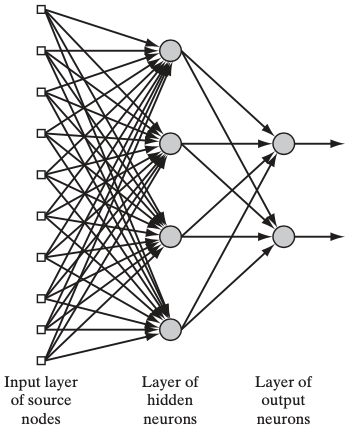
\includegraphics[width = 0.6 \linewidth]{images/netwrok structure.png}
    \centering
    \caption{Struttura di una rete neurale a più livelli.}
    \label{network structure}
\end{figure}
Una componente importante, riguarda la presenza di un insieme di valori 
$w=(w_{j1}, \dots, w_{jm})$ chiamati pesi. Ogni peso è rappresentato da un numero reale 
che riflette il grado di importanza di una data connessione, tra due neuroni, in 
una rete neurale. I pesi possono subire dei cambiamenti in base alla tipologia 
di apprendimento della rete. Una buona configurazione dei pesi riduce l'errore di 
predizione e pertanto migliora l'output del modello. Riprendendo il discorso 
dei neuroni, McCulloch e Pitts  \cite{Chakraverty2019} definirono un modello matematico in grado di 
rappresentarli. In particolare, il compito di ogni singolo neurone è rappresentato 
nella figura (\ref{neural neuron}).
\begin{figure}
    \centering
    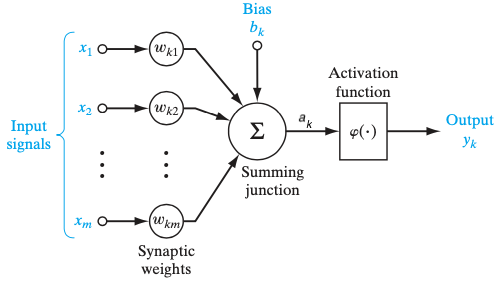
\includegraphics[width = \linewidth]{artificial neuron.png}
    \centering
    \caption{Neurone artificiale.}
    \label{neural neuron}
\end{figure}
Da come possiamo notare, un neurone è una semplice funzione non lineare 
che riceve in input una serie di input $X_{ji}$ e produce in output una variabile $y_k$. 
Il calcolo dell'output, di ogni singolo neurone, è composto da una sommatoria 
degli input, di segno positivo o negativo, moltiplicati prima con i corrispettivi 
pesi e successivamente sommati con una variabile, chiamata bias (pregiudizio), 
che corrisponde alla soglia di attivazione del neurone.
\begin{equation}\label{artificial}
    a_j = \sum_{i=0}^m w_{i}x_i + b_i 
\end{equation}
Una soglia è utile per determinare se l'informazione in ingresso “$x$” debba essere 
elaborata oppure scartata. Di solito vi è sempre un input $X_0=1$ che renderebbe 
il bias $ b_i $ uguale uguale al primo peso $W_0$, pertanto la formula (\ref{artificial}) può anche 
essere scritta come:
\begin{equation}\label{artificial without bias}
    a_j = \sum_{i=0}^m w_{i}x_i
\end{equation}
Per poter determinare il valore $y$, dopo aver ottenuto “$a$”, si utilizza una “\emph{funzione 
di attivazione}” non lineare $\varphi(\cdot)$:
\begin{equation}\label{activation function 1}
    y_j = \varphi(a) = \varphi\left(\sum_{i=0}^m w_ix_i\right)
\end{equation}
L'uscita $y$ determinerà l'attivazione del prossimo neurone. Se il valore ricevuto è 
maggiore di zero, allora il neurone si attiverà, altrimenti resterà spento.
\begin{equation}\label{activation function 2}
    y_j = \left\{
        \begin{array}{rl}
        1 & \mbox{if } a_j \geq 0 \\
        0 & \mbox{if } a_j < 0
        \end{array}
        \right.
\end{equation}
Esistono varie funzioni di attivazione, diverse sono elencate in figura (\ref{activation functions}).
\begin{figure}
    \centering
    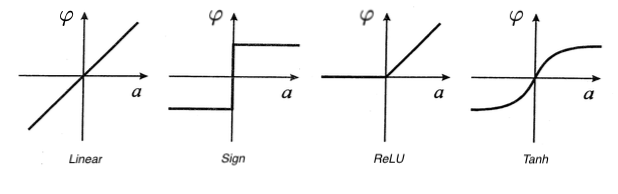
\includegraphics[width = \linewidth]{activation functions.png}
    \centering
    \caption{Varie funzioni di attivazione.}
    \label{activation functions}
\end{figure}
Grazie a questa massiccia interconnessione, le reti neurali artificiali sono in 
grado non solo di imitare il comportamento del cervello umano ma anche di 
svolgere diversi compiti grazie a una opportuna fase di apprendimento. 

\section{Algoritmi di apprendimento}
Lo scambio di dati tra i vari neuroni consente alla rete neurale di poter generalizzare 
anche con dati mai visti nel training set. Questo processo prende il nome di 
“\emph{Apprendimento}”. L'apprendimento di un modello di rete è tipicamente effettuato 
a partire da un insieme di dati di addestramento chiamato training test. All'interno 
di questi insiemi abbiamo la presenza di esempi formati da coppie $(x^j, y^j)$, con 
$j=1, \dots ,n$, dove $y^j$ sta a rappresentare il valore di output desiderato in funzione 
del dato di input $x^j$. Per ricavare il valore target è necessario ricercare gli 
opportuni valori dei pesi, indispensabili a minimizzare l'errore commesso. La 
quantità dell'errore commesso, dal singolo neurone $j$, è esprimibile mediante (\ref{error function}):
\begin{equation}\label{error function 1}
    \emph{$e_j$}=(\hat{y}_j-y_j)^2
\end{equation}
Si può osservare che il calcolo di (\ref{error function 1}) è riconducibile alla somma dei quadrati 
residua tra il valore stimato $\hat{y}_j$ e quello desiderato $y_j$. L'errore totale derivato da 
tutta la rete è calcolabile prendendo in considerazione la \emph{Funzione di Errore}, a 
volte chiamata anche di \emph{Costo}, esprimibile dal calcolo della seguente formula:
\begin{equation}\label{error function}
    \emph{$E$}=\frac{1}{2}\sum_{j=1}^me_j
\end{equation}
dove $m$ rappresenta il numero totale di neuroni presenti nell'output layer.
La funzione di errore $E$ risulta essere molto importate nella fase di apprendimento in quanto misura la distanza 
dalla soluzione ottimale. In generale, la funzione di errore ha diversi minimi (Fig. \ref{minimum and maximum})
\begin{figure}
    \centering
    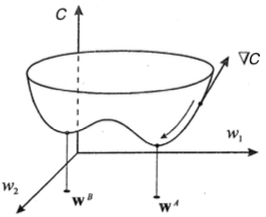
\includegraphics[width = 0.7\linewidth]{cost-function.png}
    \centering
    \caption{Esempio di minimo globale ($w^A$) e locale ($w^B$).}
    \label{minimum and maximum}
\end{figure}
Per ottenere un valore della funzione relativamente basso, l'obiettivo è racchiuso 
nella ricerca del minimo globale. Tale ricerca avviene in maniera iterativa, partendo 
da dei pesi a valori casuali, fino a definirne dei valori fissi. La ricerca dei pesi 
ottimali avviene mediante calcolo delle derivate parziali sulla funzione di errore, 
ovvero del suo vettore gradiente $\nabla{E}$ (\ref{gradient vector}). 
\begin{equation}\label{gradient vector}
    \nabla{E}[\vec{w}]\equiv\left[\frac{\partial E}{\partial w_{0}}, \frac{\partial E}{\partial w_{1}}, \dots, \frac{\partial E}{\partial w_{j}}\right]
\end{equation}
Questo vettore è utile a definire la direzione ed il verso della funzione di errore, 
in base al set di pesi considerato. Il calcolo delle derivate viene svolto da una ben 
nota tecnica presente allo stato dell'arte, chiamata \emph{Back Propagation} (discussa 
nella sezione \ref{BP} di questo elaborato). Una rete neurale artificiale può avere vari 
tipi di apprendimento: \emph{Supervisionato, Semi-Supervisionato, Non-Supervisionato} 
e con \emph{Rinforzo}. La scelta di quale usare dipende dalla tipologia della rete e dal 
suo campo di applicazione.

\subsection{Apprendimento Supervisionato}
In questa tipologia di apprendimento, l'input fornito alla rete contiene una serie di 
dati etichettati. L'apprendimento supervisionato è solitamente utilizzato sia nel 
conteso della classificazione, dove  si vuole mappare le etichette di input a quelle 
di output, che nel contesto della regressione, dove si mira a mappare l'input a un 
output continuo. La corretta associazione comporta una buona generalizzazione 
da parte del modello. L'apprendimento migliora grazie ad una continua variazione 
dei pesi. Questo tipo di apprendimento è svolto utilizzando la tecnica della 
\emph{Back-Propagation}. La complessità di questo tipo di apprendimento deriva dalla 
quantità di dati presenti nel training set. Affinché la rete riesca a generalizzare al 
meglio, il training set dev'essere composto da un numero di esempi adeguato. La 
giusta quantità di esempi è utile a prevenire spiacevoli situazioni di underfitting o 
di overfitting della rete. In questa categoria di apprendimento fanno parte diversi metodi deep 
learning, incluse le \emph{Deep Neural Networks (DNN)}, le \emph{Convolutional Neural 
Networks (CNN)}, le \emph{Recurrent Neural Networks (RNN)} come le \emph{Long 
Short-Term Memory (LSTM)} \cite{LSTM}.

\subsection{Apprendimento Non-Supervisionato}
Quando una rete neurale è sottoposta ad un simile apprendimento, questa 
riceve in input dei dati privi di etichettatura o non strutturati. Lo scopo 
della rete, o del modello, è quello di estrarne una rappresentazione e creare 
dei cluster rappresentativi. Ci sono delle tecniche a supporto di questa 
tipologia di apprendimento, una fra queste è la riduzione della dimensionalità 
che è applicata in fase di pre-elaborazione delle features avente l'obiettivo di 
eliminare il rumore dai dati quando questi sono presenti in grandi quantità. 
Nel dominio dell'apprendimento non supervisionato fanno parte quei metodi 
utili per effettuare il clustering e la riduzione della dimensionalità non lineare, 
come gli \emph{Auto Encoders (AE)} e le \emph{Generative Adversarial Networks (GAN)}. 
Anche le RNN, come le LSTM, vengono utilizzate anche per l'apprendimento 
non supervisionato in molti domini applicativi.  

\subsection{Apprendimento Semi-Supervisionato}
Un set di input composto da dati etichettati e non, costituisce un sistema di apprendimento 
semi-supervisionato. Questa tipologia di apprendimento rappresenta 
un sistema che si interpone tra i due precedentemente spiegati. I modelli che fanno 
uso di questo approccio di solito utilizzano una piccola quantità di dati etichettati 
e una grande quantità di dati non etichettati. Tale apprendimento porta alla 
creazione di un modello più flessibile rispetto a quello ottenuto dall'apprendimento 
supervisionato. Nel dominio semi-supervisionato, come tipologia di reti troviamo le GAN, le RNN, incluse le LSTM.

\subsection{Apprendimento con Rinforzo}
L'ultimo tipo di apprendimento automatico è chiamato Apprendimento con 
Rinforzo. Il suo scopo è quello di costruire un sistema, comunemente chiamato 
\emph{agente}, che abbia l'obiettivo di migliorare le sue performance interagendo con 
l'ambiente che lo circonda. Il miglioramento dell'intero sistema avviene mediante 
dei feedback chiamati appunto rinforzi. Quest'ultimi non hanno nulla a che fare 
con etichette o valori di verità, ma rappresentano un livello di qualità delle azioni 
intraprese dal sistema. Pertanto, differentemente da un sistema supervisionato, 
non ci sono mappature tra l'input e l'output. In questo dominio fanno parte le \emph{Deep Q-Netwroks (DQN)}.


\subsection{Algoritmo di Back-Propagation}\label{BP}
Il termine \emph{Back-Propagation} è stato introdotto una prima volta quando si è 
trattato l'argomento dell'apprendimento Supervisionato. Una prima definizione 
del termine venne data nel 1986 in \cite{03}. L'algoritmo di Back-Propagation agisce 
durante la fase di training del modello, che a sua volta si suddivide in due fasi:
\begin{enumerate}
    \item \emph{Fase in avanti (forward)}: i dati si propagavano dai neuroni di input fino 
    a raggiungere i neuroni di output. I pesi sono fissati e i cambiamenti sono 
    limitati.
    \begin{figure}
        \centering
        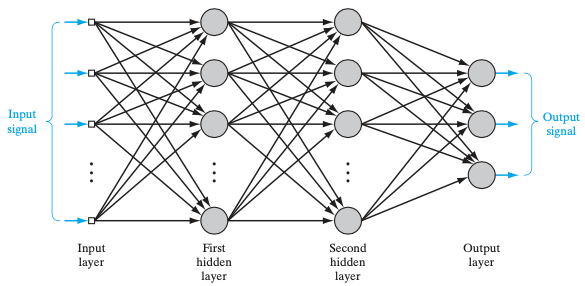
\includegraphics[width = \linewidth]{feedforward.png}
        \centering
        \caption{Esempio fase di propagazone dei dati in avanti di una rete \emph{feedforward}.}
        \label{feedforward net}
    \end{figure}
    \item \emph{Fase in indietro (backward)}:  si confronta il risultato ottenuto, da un primo 
    step in avanti, con il risultato atteso. Tale valore rappresenterà l'errore 
    commesso, descritto in precedenza dalla funzione di errore $E$ (\ref{error function}). A questo 
    punto, tale errore si propagherà indietro nella rete. Questo meccanismo è 
    utile ad adeguare i vari pesi presenti nella rete affinché le prossime iterazioni 
    diano un errore relativamente basso (caso ottimale in cui l'output stimato è 
    simile all'output desiderato).
    \begin{figure}
        \centering
        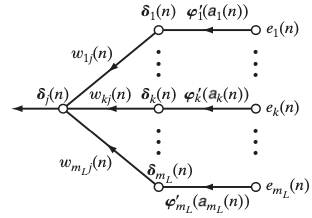
\includegraphics[width = 0.7\linewidth]{BP.png}
        \centering
        \caption{Esempio fase di retropropagazione degli errori.}
        \label{BP error}
    \end{figure}
\end{enumerate}
Sappiamo che una minima variazione ai pesi e al bias comporta allo stesso modo 
una variazione della funzione di errore E. Tralasciando un'attimo il bias, il discorso 
che segue è incentrato sulla gestione dei pesi. L'algoritmo di Back-propagation 
applica una correzione chiamata {\bfseries{Delta Rule ($\Delta{W_{ji}}$)}}  ad ogni peso $w_{ji}$, andando 
a calcolare, tramite la regola della \emph{Chain Rule} \ref{chain rule}, la derivata parziale della funzione 
di errore $E$, rispetto alla derivata della parziale del peso $w_{ji}$ in considerazione.
\begin{equation}\label{chain rule}
    \frac{\partial E}{\partial w_{ji}} = \frac{\partial E}{\partial e_{j}} 
    \frac{\partial e_{j}}{\partial y_{j}}
    \frac{\partial y_{j}}{\partial a_{j}}
    \frac{\partial a_{j}}{\partial w_{ji}}
\end{equation}
dove:
\begin{equation}\label{derivation solved 1}
    \frac{\partial E}{\partial e_{j}} = e_j
\end{equation}
\begin{equation}\label{derivation solved 2}
    \frac{\partial e_{j}}{\partial y_{j}} = -1
\end{equation}
\begin{equation}\label{derivation solved 3}
    \frac{\partial y_{j}}{\partial a_{j}} = \varphi_j^{'}(a_j)
\end{equation}
\begin{equation}\label{derivation solved 4}
    \frac{\partial a_{j}}{\partial w_{ji}} = y_i
\end{equation}
Ogni elemento definito dalla chain rule sarà utile, oltre che a formare il vettore 
del gradiente $\nabla{E}$ (\ref{gradient vector}), a determinare la direzione di ricerca all'interno dello spazio 
dei pesi, per un singolo peso $w_{ji}$. Questa operazione, in letteratura, è nominata 
come \emph{“Discesa del gradiente”}. Ricapitolando, la (\ref{chain rule}) diventa:
\begin{equation}\label{chain rule update}
    \frac{\partial E}{\partial w_{ji}} = -e_j\varphi_j^{'}(a_j)y_i
\end{equation}
Giunti a questo punto, è possibile calcolare la \emph{Delta Rule} ($\Delta{W_{ji}}$) sul peso $w_{ji}$:
\begin{equation}\label{delta rule 1}
    \Delta{W_{ji}} = -\alpha \frac{\partial E}{\partial w_{ji}}
\end{equation}
dove $-\alpha$ simboleggia un parametro, chiamato \emph{Learning Rate}, che rappresenta 
un indicatore di velocità di apprendimento della rete. Il segno negativo è utile 
per agevolare la discesa del gradiente affinché si riduca il valore della funzione di
errore $E$. Dalla (\ref{delta rule 1}) possiamo definire il \emph{gradiente locale $\delta_j$}:
\begin{eqnarray}\label{local gradient of output layer}
    \delta_j & = & \frac{\partial E}{\partial a_{j}} \nonumber \\
             & = & \frac{\partial E}{\partial e_{j}} \frac{\partial e_{j}}{\partial y_{j}} \frac{\partial y_{j}}{\partial a_{j}} \nonumber \\
             & = & e_j\varphi_j^{'}(a_j)
\end{eqnarray}
Il gradiente locale sta ad indicare i cambiamenti richiesti nei pesi e questo dipende 
dalla tipologia di neurone:
\begin{enumerate}
    \item Se il neurone \emph{j} è un neurone di output, $\delta_j$ è uguale al prodotto della derivata 
    $\varphi_j^{'}(a_j)$ e il singolo errore $e_{j}$, entrambi associati al neurone $j$ (\ref{local gradient of output layer});
    \item Se il neurone \emph{j} è un neurone nascosto, $\delta_j$ è uguale al prodotto tra la derivata 
    $\varphi_j^{'}(a_j)$ e la sommatoria dei vari $\delta$ calcolati sui neuroni posti nel layer nascosto, 
    o nel layer di output, connessi al neurone \emph{j} (\ref{local gradient of hidden neuron}).
    \begin{equation}\label{local gradient of hidden neuron}
        \delta_j = \varphi_j^{'}(a_j)\sum_{k}\delta_kw_{kj}
    \end{equation}
\end{enumerate}
Sostituendo in (\ref{chain rule update}) la (\ref{local gradient of output layer}), possiamo modificare la (\ref{delta rule 1}) in:
\begin{equation}\label{delta rule 2}
    \Delta{W_{ji}} = -\alpha \delta_jy_i 
\end{equation}
Infine, grazie alla definizione della \emph{Delta Rule}, nell'iterazione $n+1$ sarà possibile 
aggiornare il peso $w_{ji}$ in questione, rispetto all'iterazione $n$ precedente:
\begin{equation}\label{weight change}
    w_{ji}(n+1) = w_{ji}(n)+\Delta{w_{ji}(n)}
\end{equation}
In precedenza, si era preferito mettere da parte il concetto di bias per concentrarci 
maggiormente sui pesi. Essendo la funzione di errore sensibile anche al cambiamento 
del bias, l'algoritmo di back-propagation ha lo scopo di aggiornare anche i 
vari bias esistenti integrando, nel vettore gradiente $\nabla{E}$, le derivate parziali della 
funzione di Errore rispetto al bias $b$:
\begin{equation}\label{gradient vector with bias}
    \nabla{E}[\vec{b}]\equiv\left[\frac{\partial E}{\partial b_{0}}, \frac{\partial E}{\partial b_{1}}, \dots, \frac{\partial E}{\partial b_{j}}\right]
\end{equation}
I successivi calcoli sono identici a quelli dell'aggiornamento dei pesi. Il processo 
di back-propagation avviene in maniera iterativa e si ferma quando vengono 
soddisfatte le seguenti caratteristiche:
\begin{enumerate}
    \item Raggiungimento del numero massimo di epoche;
    \item L'errore è più basso della soglia;
    \item Non vi è nessun cambiamento dei pesi.
\end{enumerate}

\section{Tipologie di reti neurali}
Esistono diverse tipologie di reti neurali, tra queste abbiamo:
\begin{enumerate}
    \item \emph{Feed Forward Neural Networks (FNN)}
    \item \emph{Deep Neural Networks (DNN)}
    \item \emph{Convolutional Neural Netoworks (CNN)}
    \item \emph{Recurrent Neural Networks (RNN)}
    \item \emph{Generative Adversarial Networks (GAN)}
\end{enumerate}
Nel seguente elaborato verranno trattate principalmente le reti neurali convoluzionali 
ma, prima di introdurle, al fine di capire il loro funzionamento, è necessario 
introdurre prima le reti neurali feed-forward, dette anche reti neurali a catena 
aperta.

\subsection{Feed Forward Neural Networks}
Per facilitare la comprensione del funzionamento di una comune rete neurale, 
si potrebbe partire dallo studio del comportamento di una feed-forward neural 
network. Questa tipologia di rete può essere vista come una funzione matematica 
non lineare capace di trasformare dei dati di input $x=(x_1, \dots, x_m)$, in dati in 
output $y=(y_{j1}, \dots, y_{jn})$. Quello che accade è quindi una transizione delle variabili 
indipendenti ($X_j$) in variabili dipendenti($Y_j$). Possiamo quindi considerare la 
rete come una funzione nella forma $y = y(x;w)$, dove $y$ sta a rappresentare una funzione di $x$ 
e che a sua volta è parametrizzata da $w$. In una rete feed-forward, il 
processo di calcolo è unilaterale, ovvero procede solamente in avanti, raggiungendo 
l'ultimo layer. Rispetto a una rete semplice, una rete feedforward può essere 
composta da più layer nascosti in cui vi sono più neuroni nascosti. L'aggiunta 
di un numero sostanziale di layer nascosti può aiutare ad estrarre statistiche di 
ordine superiore dai dati di input. Secondo \cite{04}, la presenza di più connessioni 
sinaptiche tra i neuroni, provoca una maggiore iterazione tra questi che a sua 
volta aiuta alla rete a raggiungere una prospettiva globale. Una rete che ha più di 
un layer nascosto, e quindi probabilmente con un alto numero di connessioni, in 
gergo è chiamata rete \emph{fully connected}. Al contrario, se alcuni collegamenti sono 
assenti, tale tipologia di rete viene chiamata \emph{partially connected}.

\subsection{Convolutional Neural Networks}\label{RNC}
Una rete neurale convoluzionale (CNN o ConvNet) è una tipologia di rete feed-
forward che si sta affermando come stato dell'arte per una svariata gamma di 
applicazioni nel campo della computer vision. Una loro prima diffusione avvenne 
negli anni '90 grazie a uno studio di LeCun e Boser \cite{NIPS1989_53c3bce6}. L'architettura delle CNN 
si distinguono grazie al numero di layer presenti.  La loro particolarità sta nel 
rilevare i tratti più rilevanti e di apprendere i pattern, il tutto con un alto grado di 
invariata rispetto a traslazione, ridimensionamento, inclinazione e altre forme di 
distorsione. I primi strati hanno il compito di estrarre le features di basso livello, 
come per esempio i bordi o i blob, al contrario, gli ultimi strati hanno lo scopo di 
estrarre le features di alto livello tipo i contorni, classificazione, riconoscimento 
etc. All'interno di una rete convoluzionale possiamo riconoscere due tipologie di 
neuroni:
\begin{itemize}
    \item \emph{Neuroni di elaborazione}: hanno lo scopo di elaborare una sezione specifica 
    dell'immagine, comunemente chiamata campo ricettivo, utilizzando 
    un'operazione di \emph{convoluzione};
    \item \emph{Neuroni di aggregazione}: hanno lo scopo di eseguire un'operazione di \emph{pooling}.
\end{itemize}
I neuroni contenuti in uno strato adibito alla convoluzione, e quelli completamente 
connessi, dispongono di funzioni di attivazione e di pesi, quest'ultimi sottoposti a 
processo di aggiornamento durante la fase di apprendimento. Per quanto riguarda 
gli strati di pooling, questi non dispongo di alcun tipi di peso. Riassumendo, 
le operazioni svolte dalle CNN sono essenzialmente quattro: {\bfseries{Convoluzione}}, {\bfseries{Non 
Linearità (ReLU)}}, {\bfseries{Pooling (o Sub Sampling)}} e {\bfseries{Classificazione}} (nei layer 
fully connected). 
\begin{figure}
    \centering
    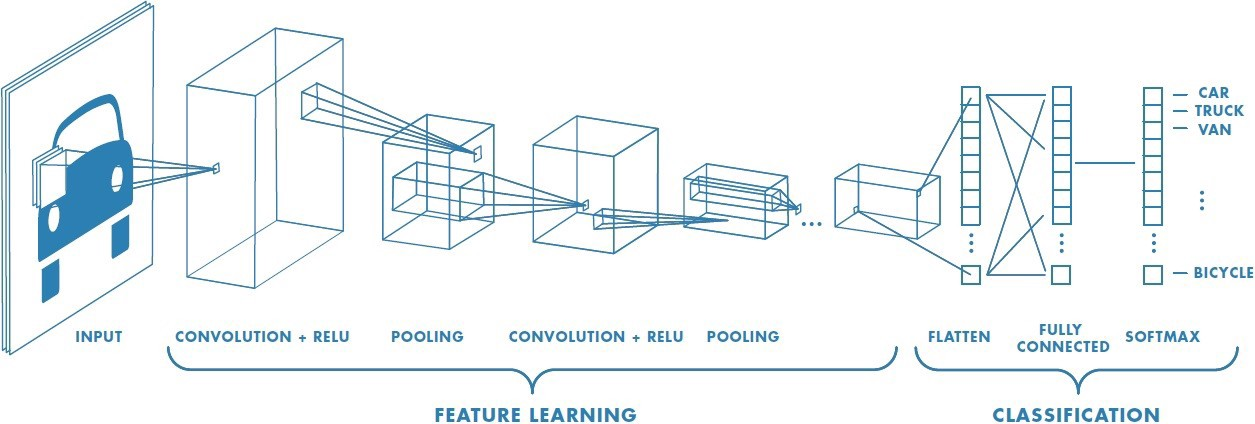
\includegraphics[width = \linewidth]{cnn complete.png}
    \centering
    \caption{Esempio di architettura di una rete CNN.}
    \label{CNN complete}
\end{figure}

\subsubsection{Convoluzione}
Lo scopo del layer di convoluzione è quello di attuare un'operazione di {\bfseries{feature 
extraction}}. In questa fase ogni neurone prende in input un campo ricettivo 
locale del layer precedente e da qui ne estrae le feature locali. Un filtro, che in 
gergo prende il nome di {\bfseries{\emph{kernel}}}, trasla sull'immagine originale con l'intenzione di 
creare una feature map mediante moltiplicazione tra i valori presenti nel filtro, 
corrispondenti ai pesi, e la regione dell'immagine in cui si trova. Di seguito, i 
valori di ogni feature map sono calcolati tramite la seguente formula:
\begin{equation}\label{sum convolution}
    G[m,n] = (f*h)[m,n] = \sum_j\sum_kh[j,k]f[m-j,n-k]
\end{equation}
dove:
\begin{itemize}
    \item $f$: immagine in input;
    \item $h$: kernel;
    \item $m,n$: indici di riga e colonna del campo ricettivo dell'immagine;
    \item $i,j$: indici di riga e colonna del kernel;
\end{itemize}
\begin{figure}
    \centering
    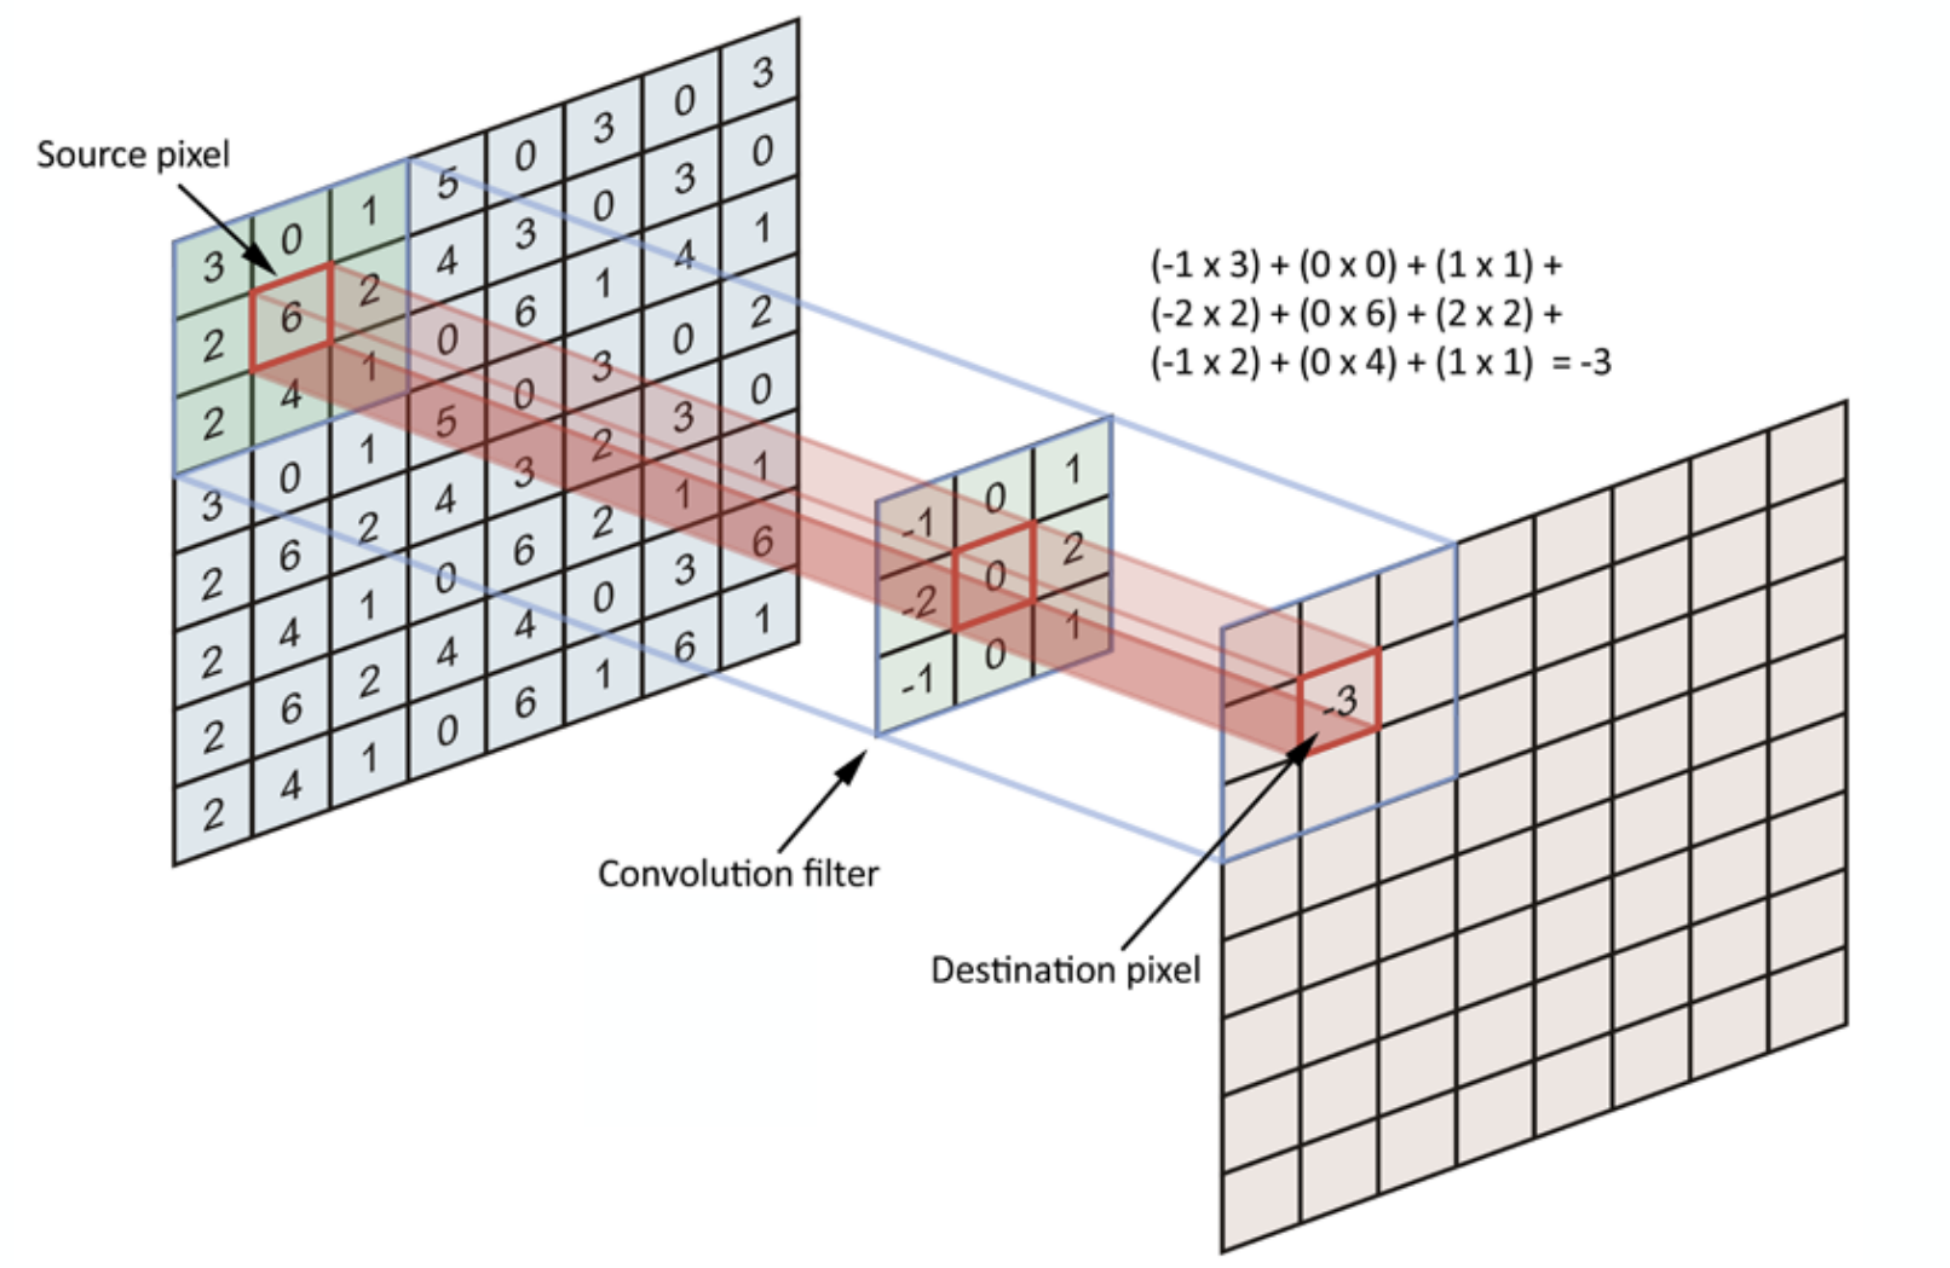
\includegraphics[width = 0.8\linewidth]{convolution.png}
    \centering
    \caption{Esempio di dimensione filtro e di campo ricettivo.}
    \label{filter dimension}
\end{figure}
Dopo aver posizionato il filtro su un campo ricettivo, vero preso ogni valore dal 
kernel e moltiplicato con i valori corrispondenti al campo ricettivo dell'immagine. 
Successivamente, il valore risultante verrà inserito nella giusta posizione della 
feature map. Il numero di feature map sarà uguale al numero di filtri applicato 
sull'immagine. La generazione di ogni feature map dipende da quattro tipi di 
parametri, detti 
\emph{iperparametri}:
\begin{enumerate}
    \item \emph{Dimensione dei filtri}: pari alla dimensione del campo ricettivo ovvero della 
    porzione dell'immagine che si vuole analizzare;
    \item \emph{Profondità (depth)}: numero di filtri “$N$” usati durante la convoluzione 
    ($H \times W \times N$). Ogni filtro produrrà una propria feature map;
    \begin{figure}
        \centering
        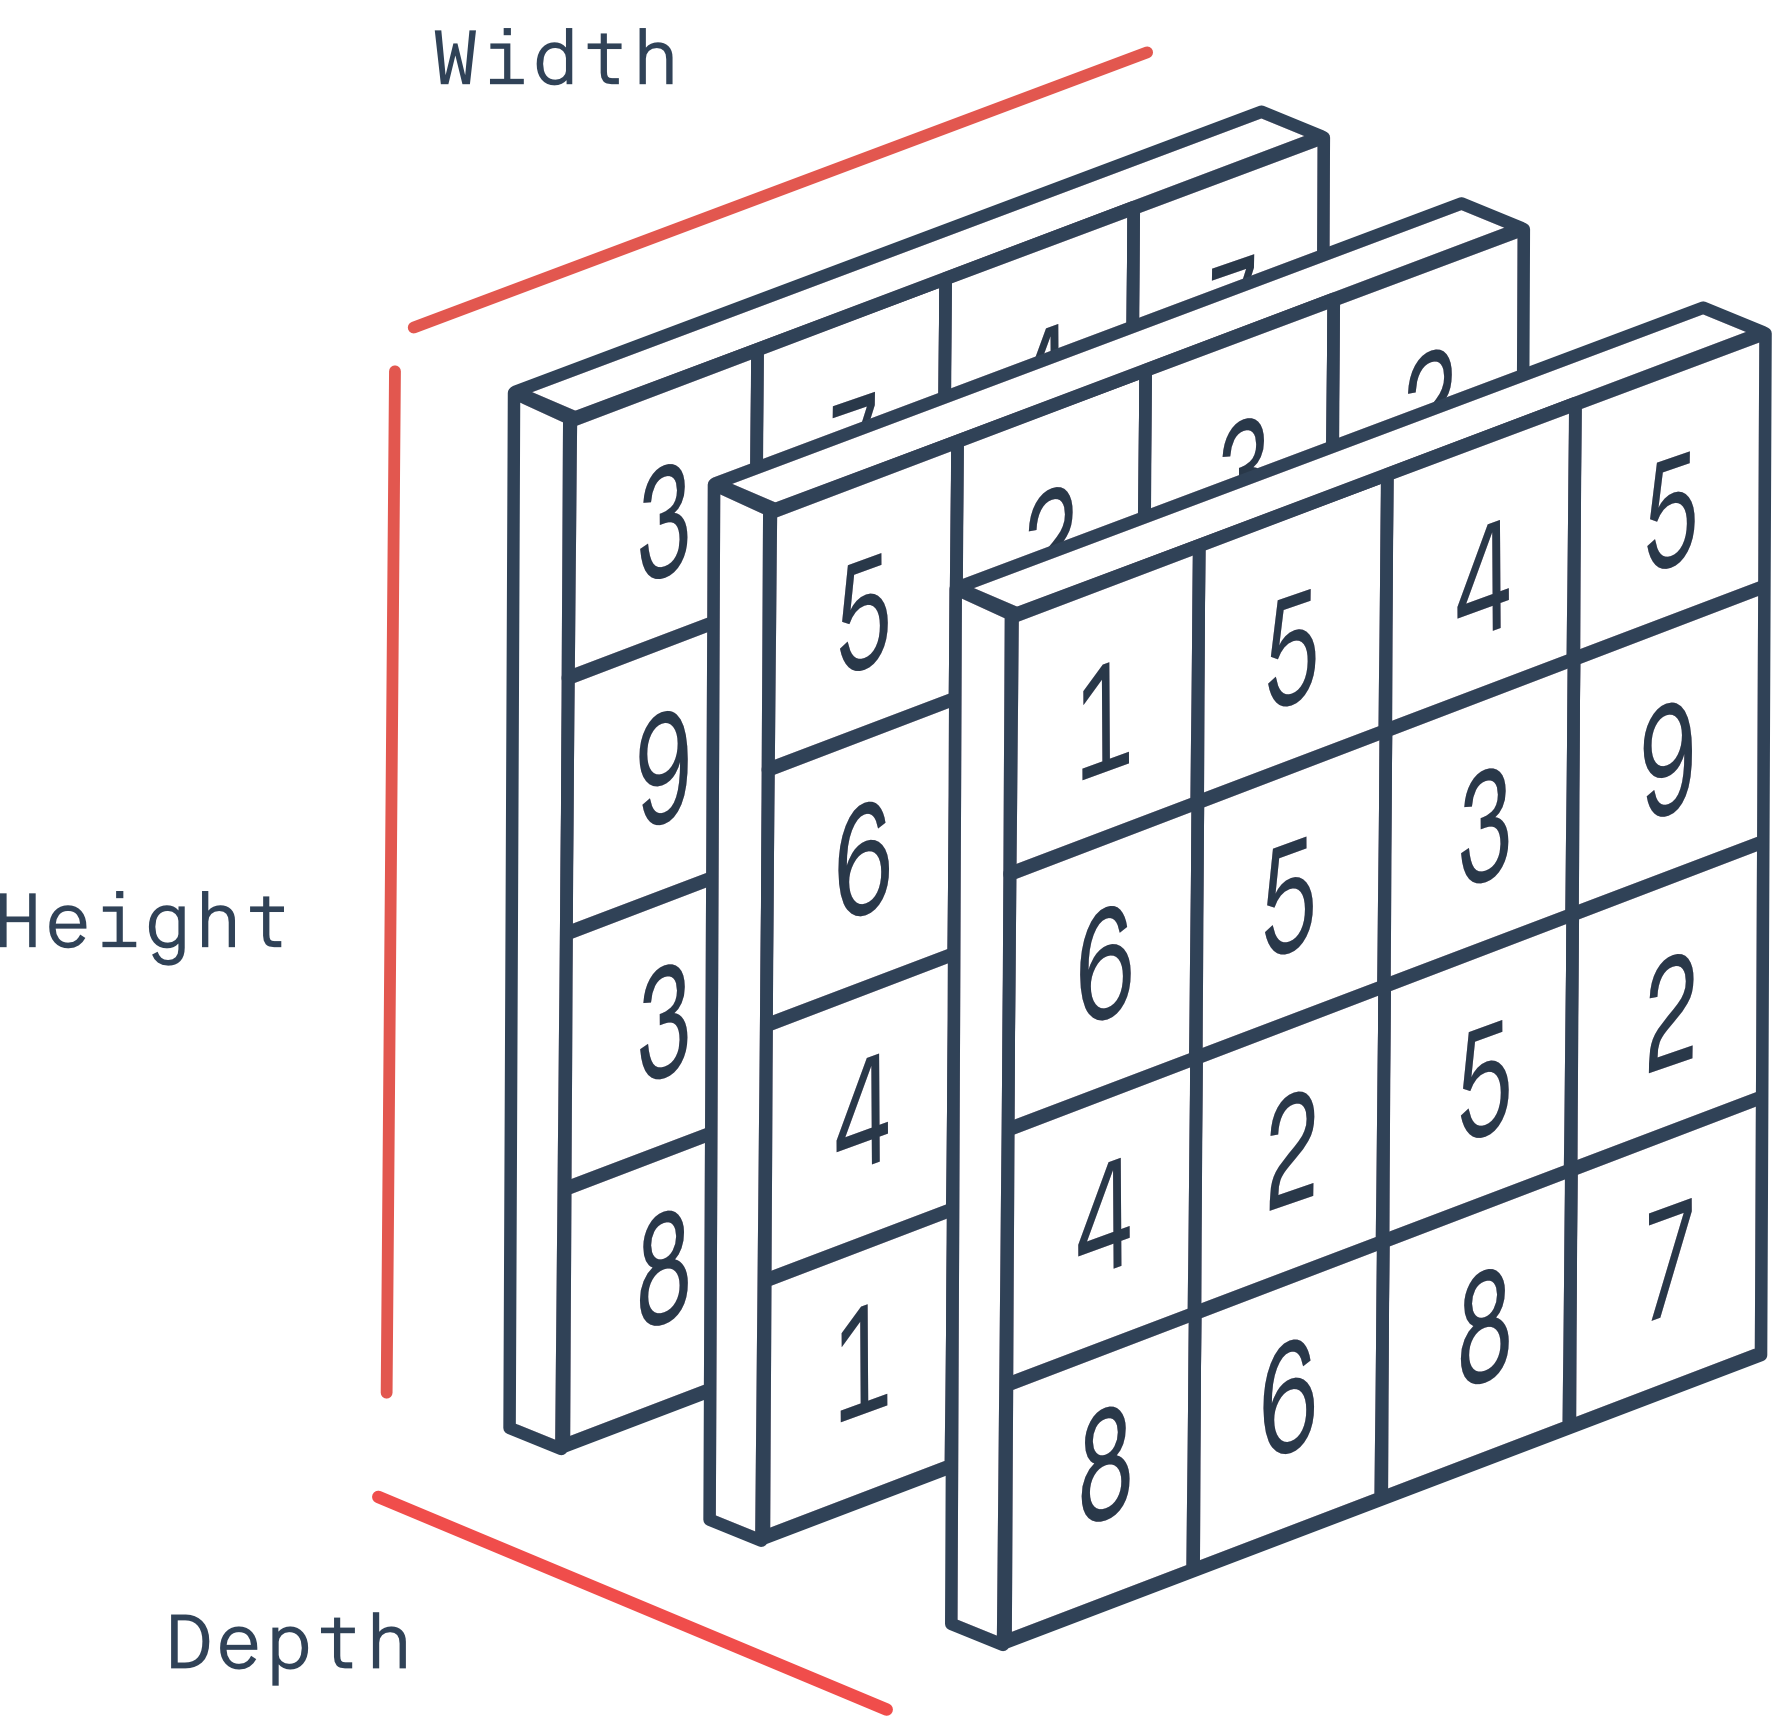
\includegraphics[width = 0.5\linewidth]{filter.png}
        \centering
        \caption{Esempio di profondità composto da più filtri.}
        \label{filters depth}
    \end{figure}
    \item \emph{Passo (stride)}: rappresenta il numero di pixel su cui viene fatto traslare il 
    kernel ogni volta che esegue una moltiplicazione. Per ottenere una buona 
    feature map è consigliato avere un valore di stride relativamente basso;
    \begin{figure}
        \centering
        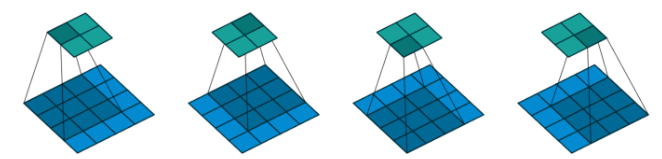
\includegraphics[width = \linewidth]{stride.png}
        \centering
        \caption{Esempio convoluzione con kernel=3x3 e stride=1.}
        \label{stride}
    \end{figure}
    \item \emph{Riempimento (Padding)}: affinché venga generata una corretta feature map 
    di dimensioni pari ($padding=1$) o maggiore ($padding>1$) a quella dell'immagine 
    di partenza, la matrice dell'immagine deve essere riempita di valori uguali, 
    esempio di zeri, presso le sue estremità.
    \begin{figure}
        \centering
        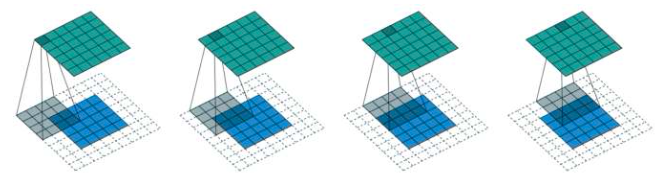
\includegraphics[width = \linewidth]{padding and stride.png}
        \centering
        \caption{Esempio convoluzione con kernel=4x, padding=2 e stride=1.}
        \label{padding e stride}
    \end{figure}
\end{enumerate}
La scelta degli iperparametri non è standard ma dipende maggiormente dalla 
tipologia dei dati a disposizione.

\subsubsection{Rectified Linear Unit (ReLU)}
Ogni feature map, dopo la convoluzione, è composta da dei valori positivi e negativi. 
Come brevemente accennato in (\ref{Reti neurali}), esistono varie funzioni di attivazione che, in 
base all'input ricevuto, decidono se attivare o disattivare un neurone. La 
funzione di attivazione maggiormente usata è la ReLU (Rectified Linear Unit). 
Questa funzione esegue delle operazioni non lineari ponendo a zero tutti i valori 
negativi e lasciando invariati i valori positivi (Fig. \ref{relu}), generando in questo modo delle 
attivazioni sparse.  L'operazione prende il nome di element-wise su tutti i pixel. 
L'implementazione di questa funzione, rispetto alle sue concorrenti, è utile ad accelerare 
il processo di apprendimento (backpropagation) del modello semplificando 
le operazioni nei vari layer.
\begin{figure}
    \centering
    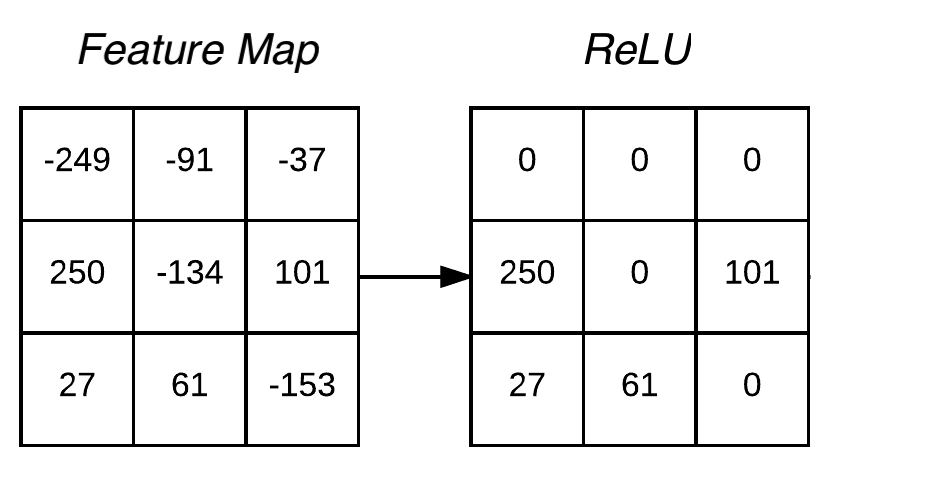
\includegraphics[width = 0.8\linewidth]{relu.png}
    \centering
    \caption{Esempio funzione di attivazione ReLU sui valori di una feature map.}
    \label{relu}
\end{figure}
Rispetto alla sigmoide, la funzione ReLU pone a zero la derivata di un numero 
negativo, mentre per i numeri positivi la derivata è uguale a uno evitando la 
saturazione del gradiente.

\subsubsection{Pooling}
La tecnica di Pooling, chiamata anche di subsampling o downsamping, ha il 
compito di ridurre la dimensionali di ogni feature map mantenendo però le 
informazioni più importanti. Il funzionamento di basa nel far scorrere una finestra, 
senza alcun tipo di valore o peso al suo interno, di dimensione inferiore rispetto 
alla grandezza della feature map, con lo scopo di aggregare i valori sottostanti. 
Esistono varie operazioni di aggregazione, le più comuni sono: somma, massimo, 
minimo e media. Così come la convoluzione, anche qui gli iperparametri Stride 
e Kernel size, entrambi solitamente uguale a 2, sono fondamentali al fine di gestire 
la finestra sovrastante. Ogni neurone, nello strato di pooling, è connesso a un 
numero limitato di neuroni nello strato precedente
\begin{figure}
    \centering
    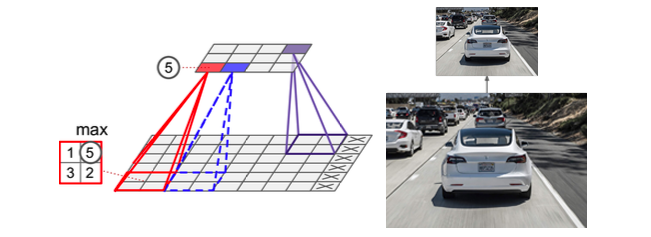
\includegraphics[width = \linewidth]{pooling tesla.png}
    \centering
    \caption{Esempio funzione di operazioni di pooling su una feature map.}
    \label{pooling}
\end{figure}
In (Fig. \ref{pooling}), applicando al funzione di \emph{Max-Pooling} al campo ricettivo in 
basso a sinistra, verrà selezionato il valore 5 che sarà propagato al prossimo 
layer. Avendo uno stride pari a 2, la matrice prodotta avrà una dimensione 
uguale alla metà della matrice di partenza (subsamplig),  che in questo caso è 
stata arrotondata per difetto. La riduzione delle dimensioni a sua volta riduce 
il numero di operazioni di calcolo, l'occupazione della memoria e il numero di 
parametri, limitando anche il rischio di overfitting in quanto si ha un numero 
minore di paramenti da apprendere. La funzione di Max-Pooling introduce quella che viene 
chiamata \emph{invarianza}, fattore importante che non permette ai cambiamenti di 
stravolgere il risultato finale, aggiungendo robustezza ai dati.

\subsubsection{Fully Connected}
Il layer \emph{Fully Connected (FC)} è una tradizionale \emph{Multilayer Perceptron (MLP)} 
che include una funzione di attivazione \emph{Softmax} nel layer di output. Lo scopo di 
tale layer è quello di utilizzare le feature estratte, dagli strati precedenti, in modo 
da predire le loro classi di appartenenza precedentemente fornite nel training 
set. Un vettore di numeri reali conterrà tutte le predizioni che, se sommate tra 
loro, produrranno un valore uguale a uno. Quest'ultimo passaggio sarà possibile 
grazie all'utilizzo di una funzione chiamata Softmax, posta alla fine dell'intera 
rete convoluzionale, che è in grado di “schiacciare” un vettore K-dimensionale 
a valori reali arbitrali, in un vettore K-dimensionale a valori reali, compresi nel 
range $(0,1)$. 

\subsection{Recurrent Neural Networks}
A differenza delle CNN, le Recurrent Neural Networks consentono operazioni 
su una sequenza di valori temporali (\emph{Time series}). Uno dei modelli 
migliori rappresentante le RNN, venne introdotto da Gers and Schmidhuber, 
intitolato Long Short-Term Memory (LSTM) \cite{LSTM}. La RNN rappresenta 
una classe di reti artificiali avente lo scopo di effettuare delle previsioni 
su fattori futuri, come per esempio le variazioni di prezzo di un bene, la 
traiettoria di un veicolo etc. In particolare, la peculiarità di queste reti 
sta nel trattare un input di lunghezza arbitraria differenziandosi da altre 
architetture che richiedono un input a lunghezza prefissata (es: CNN). Nelle 
reti precedentemente introdotte, l'input veniva trasportato dallo strato di 
input verso lo strato di output. A differenza di queste, le RNN hanno una 
connessione simile alle CNN che li permette di retro propagare i dati in direzione 
opposta. Per capire meglio, immaginiamo che una RNN sia composta 
da un solo neurone che, all'istante di tempo $t$, prende in input un dato $X_t$, 
lo elabora e produce un output $Y_{t+1}$ che lo re-invia a se stesso creando una specie di loop (Fig. 
(\ref{neuron-rnn})).
\begin{figure}
    \centering
    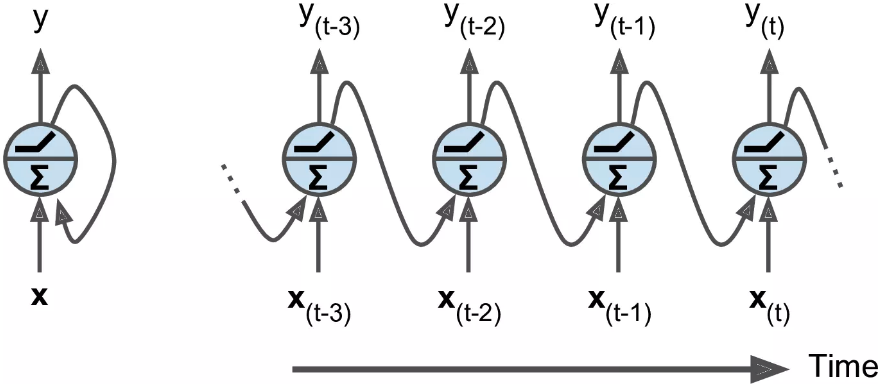
\includegraphics[width = \linewidth]{RNN.png}
    \centering
    \caption{Esempio di neurone in una Recurrent Neural Network. A destra viene mostrata la struttura e i compiti di un singolo neurone nell'istante di tempo $t$. A sinisitra invece viene mostrata una sequenza di azioni svolte dallo stesso neurone in una sequenza temporale.}
    \label{neuron-rnn}
\end{figure}
Seguendo questa ricorsione, nell'istante di tempo successivo, ogni nuovo input $X_t$ corrisponderà 
all'output $Y_{t-1}$ e così via.  Se considerassimo ogni output, corrispondente all'istante di 
tempo $t$, in funzione di tutti gli input del precedente istante di tempo, allora possiamo 
considerare questo concetto di ricorrenza come un concetto di memoria della rete. Ogni 
neurone quindi rappresenta una cella di memoria capace di preservare qualche stato nel 
tempo. Questo stato, denotato con $h_t$ (dove h sta per hidden), è una funzione che dipende:
\begin{itemize}
    \item dall'input appartenente a un determinato istante di tempo $t$;
    \item dal suo stato $h$ precedente.
\end{itemize}
\begin{equation}
    h_t = f(h_{t-1}, x_t)
\end{equation}
\begin{figure}
    \centering
    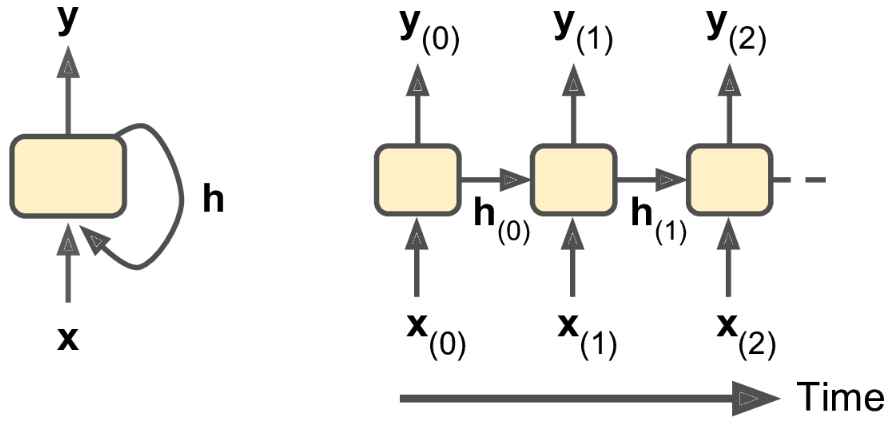
\includegraphics[width = 0.9\linewidth]{state RNN.png}
    \centering
    \caption{Esempio di stato $h$ di un neurone in una RNN.}
    \label{state-neuron-rnn}
\end{figure}
Individualmente, l'output di ogni neurone corrisponde allo stato stesso 
(Fig. (\ref{state-neuron-rnn})). Esistono diverse versioni di RNN che differiscono 
in base alla sequenza di input e di output. Distinguiamo almeno quattro versioni:
\begin{enumerate}
    \item \emph{Sequence to Sequence}: utile per quei problemi che richiedono il calcolo 
    di una previsione futura basandosi sul una serie temporale di dati;
    \item \emph{Sequence to Vector}: tipologia di RNN che prende una sequenza di 
    valori input e tiene in considerazione solo un valore di output, ignorando 
    tutti gli output intermedi;
    \item \emph{Vector to Sequence}: al contrario del sequence-to-vector, questa volta 
    si fornisce un solo input e si considerano tutti gli output prodotti ad 
    ogni istante di tempo;
    \item \emph{Delayed sequence to sequence}: in questa tipologia abbaino un'architettura 
    RNN composta da una prima parte chiamata \emph{Encoder} che 
    effettua operazioni di tipo sequence-to-vector ed una seconda parte 
    chiamata \emph{Decoder} che si occupa di effettuare la vector-to sequence. 
    Questa tipologia di rete è molto utilizzata per effettuare le 
    traduzioni linguistiche. 
\end{enumerate}

\subsection{Generative Adversarial Networks}
Le Generative Adversarial Networks (GAN) vennero proposte da Goodfellow 
nel 2014 \cite{GAN}. Questa famiglia di reti appartiene all'approccio non 
supervisionato ma vengono utilizzate anche a supporto dei sistemi con 
apprendimento rinforzato. Gli utilizzi di una GAN riguardano la stima dei 
modelli generativi attraverso un processo composto da due reti indipendenti, 
una generativa (G) e l'altra discriminatoria (D). La prima ha il compito di 
catturare una distribuzione originale mentre la seconda si occupa di stimare 
la probabilità che un dato provenga dal dataset di riferimento anzichè dalla 
prima rete G. Spiegata in altri termini, la prima rete viene sottoposta a 
un processo di training atto a massimizzare la probabilità che la rete D 
sbagli la sua predizione. Tramite un continuo processo di back and forward, 
fra il generatore che fornisce dei dati inizialmente casuali e il discriminante 
che rilascia un feedback che attesti la loro veridicità, le reti di tipo GAN 
possono essere utilizzate per vari scopi. Fra questi ricadono i metodi di 
Image enhancement, predizione del traffico stradale a supporto dei veicolo 
a guida autonoma \cite{GAN-ADAS}, generazione di volti fasulli e generazione di dipinti 
simili a quelli originali. Il discriminante elabora l'immagine ricevuta dal 
generatore e produce una probabilità D(x) che ne attesti la sua reale autenticità 
con l'immagine del training set. A questo punto, lo scopo del 
generatore è quello appunto di generare più versioni modificate di questa 
immagine fino a quando la probabilità D è maggiore di una soglia che porti 
il discriminante a considerare l'immagine come autentica. Un esempio del 
lavoro svolto da una rete GAN è illustrato nella FIgura (\ref{gan-nn})
\begin{figure}
    \centering
    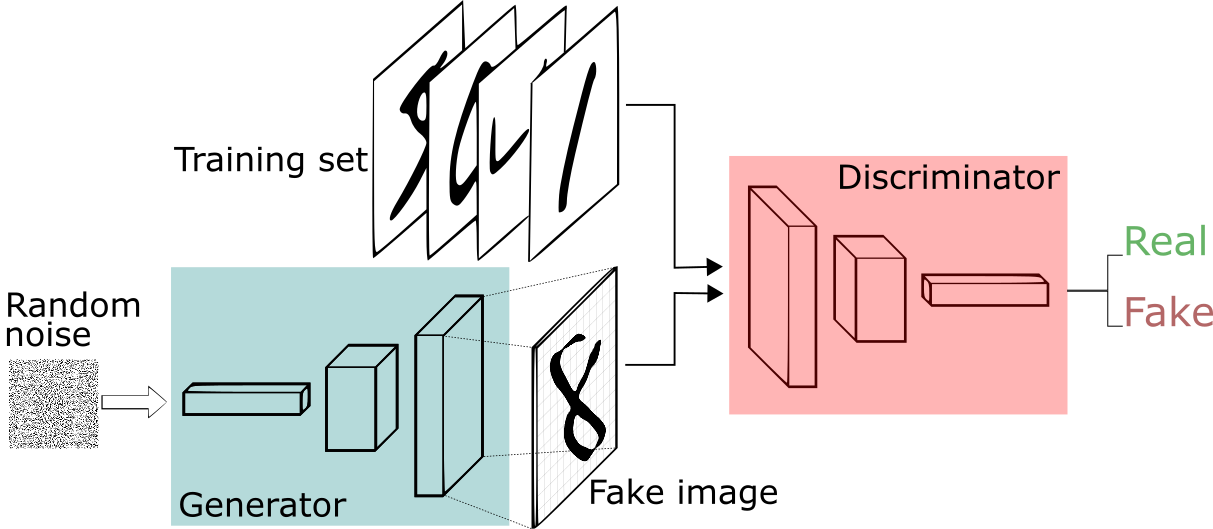
\includegraphics[width = 0.9\linewidth]{GAN.png}
    \centering
    \caption{Esempio di generatore e discriminante in una rete GAN.}
    \label{gan-nn}
\end{figure}


\section{Utilizzi delle reti neurali}
L'introduzione delle reti neurali, sia nel campo della computer vision che del deep 
learning, ha portato vari benefici nel risolvere problemi complessi nella vita reale. 
Il supporto offerto da questi sistemi è basato su tecniche di elaborazione delle 
immagini in grado di estrarre diverse informazioni utili per un determinato scopo. 
I task principali, eseguiti su un'immagine, possono essere:
\begin{itemize}
    \item \emph{Image classification}: viene effettuata un'analisi dell'immagine con lo scopo 
    di assegnare un'etichetta in base al suo contenuto;
    \item \emph{Object detection}: analisi degli elementi presenti all'interno di un'immagine;
    \item \emph{Image segmentation}: estrazione di regioni di interesse che identificano il 
    target in base al contesto;
    \item \emph{Face recognition}: basato sul riconoscimento facciale delle persone;
    \item \emph{Action recognition}: analisi incentrata sull'identificazione e sulla descrizione 
    di azioni compiute da parte di soggetti che interagiscono nel tempo e nello 
    spazio circostante;
    \item \emph{Visual Relationship Detection}: analisi mirata alla relazione che intercorre 
    tra gli oggetti presenti nell'immagine;
    \item \emph{Emotion Recognition}: processo atto a identificare le emozioni umane mediante 
    vari fattori come quello vocale e/o visivo;
    \item \emph{Image editing}: analisi delle immagini che portano l'algoritmo a riconoscere 
    le parti più rilevanti di un'immagine, come per esempio quelle più sensibili, 
    ed a attuare delle specifiche azioni, come ad esempio il loro oscuramento.
\end{itemize}
Il presente elaborato farà riferimento solamente alle prime tre tecniche, soffermandosi 
maggiormente sull'object detection e la semantic segmentation (branca 
dell'image segmentation).

\subsection{Object Detection}\label{OBJD}
L'object detection costituisce la base per risolvere compiti di visione complessi, 
o di alto livello, come la segmentazione, comprensione della scena, tracciamento 
degli oggetti, rilevamento degli eventi e riconoscimento delle attività. La tecnica 
di object detection supporta un ampio range di applicazioni, tra queste abbiamo 
la visione robotica, sicurezza, guida autonoma, segnali stradali, interazione uomo 
macchina, recupero delle immagini basato sui contenuti, videosorveglianza, realtà 
aumentata e ambito medico. Dal grafico \ref{obj det performance} possiamo vedere che dopo l'anno 
2012, periodo corrispondente all'introduzione del deep learning, le prestazioni 
della tecnica di object detection aumentarono notevolmente.
\begin{figure}
    \centering
    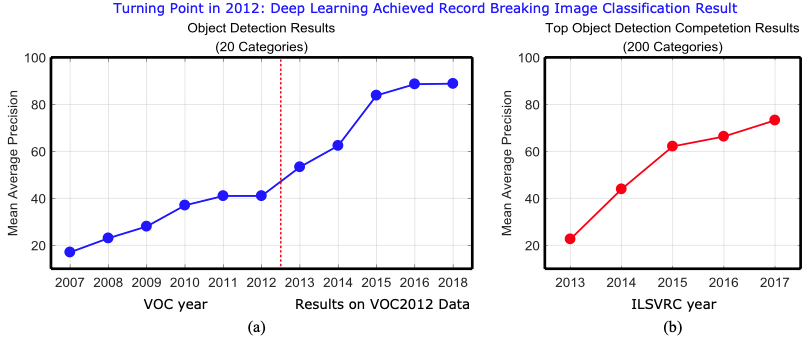
\includegraphics[width = \linewidth]{obj detection performance.png}
    \centering
    \caption{(a) Risultati object detection, in termini di mean average Precision, nelle competizioni VOC2007-2012 e (b) risultati della competizione per il rilevamento degli oggetti in ILSVRC2013-2017 su un numero di categorie maggiore}
    \label{obj det performance}
\end{figure}
Ogni oggetto è caratterizzato dalle sue proprietà come colore, forma, texture 
o altri tratti. Lo scopo della tecnica può essere visto come un problema di 
classificazione in grado di definire se un'immagine contiene un oggetto e, in caso 
affermativo, indicarne la posizione nell'immagine mediante l'utilizzo di un riquadro 
di delimitazione chiamato bounding box (Fig. \ref{object detection}). 
\begin{figure}
    \centering
    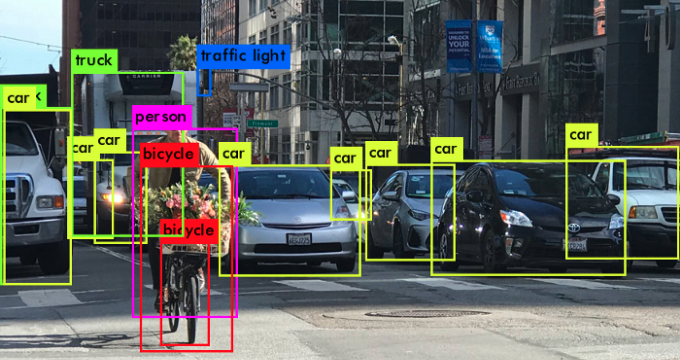
\includegraphics[width = 0.9\linewidth]{object detection.png}
    \centering
    \caption{Esempio di object detection.}
    \label{object detection}
\end{figure}
Se invece di un'immagine si sta elaborando un insieme di frame, come un video, 
allora lo scopo è quello di tracciare la posizione e  la dimensione dell'oggetto in 
tutti i frame (tecnica comunemente chiamata object tracking). Il rilevamento 
degli oggetti generici è strettamente correlato a:
\begin{enumerate}
    \item \emph{Segmentazione Semantica}: ha lo scopo di assegnare a ciascun pixel dell'immagine 
    un'etichetta corrispondente ad una classe (Fig. \ref{segmentation} (a));
    \item \emph{Instance segmentation}: tecnica che, al contrario della segmentazione semantica, 
    mira a distinguere diverse istanze appartenenti alla stessa classe di 
    oggetti (Fig. \ref{segmentation} (b)).
\end{enumerate}
\begin{figure}
    \centering
    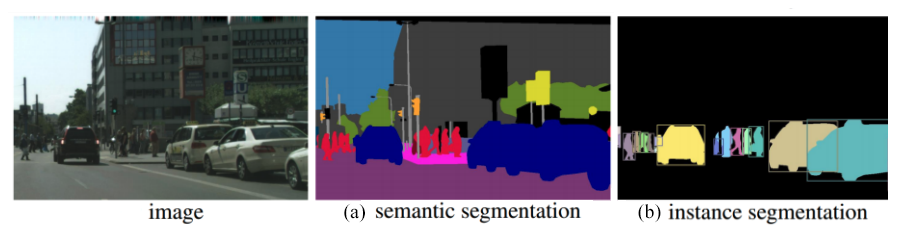
\includegraphics[width = \linewidth]{segmentation.png}
    \centering
    \caption{Problemi di riconoscimento relativi al rielvamento di automobili e pedoni: (a) Pixel-wise semantic segmentation, (b) Instance level semantic segmentation. }
    \label{segmentation}
\end{figure}
Uno dei principali obiettivi in questo campo è scegliere le feature che sono 
più caratteristiche dell'oggetto ricercato o, in altre parole, che sono altamente 
discriminanti, in modo da ottenere dei buoni risultati da parte del classificatore. Un 
aspetto fondamentale da tenere in considerazione è la complessità computazionale 
a cui i sistemi vanno incontro \cite{cyganek2013object}. I primi modelli di object detection basavano 
il loro funzionamento su delle feature estratte a mano \cite{viola2001rapid} \cite{dalal2005histograms}. Purtroppo, questi 
modelli erano molto lenti, imprecisi e non erano in grado di riconoscere i dati mai 
visti in precedenza. Le reti neurali convoluzionali (CNN) e del deep learning hanno 
cambiato il panorama della percezione visiva. Il problema di object detection è 
generalmente visto come un problema di apprendimento supervisionato. Nella 
computer vision sono stati raggiunti traguardi importanti negli ultimi dieci anni, 
tuttavia ci sono ancora grandi sfide da superare. Di seguito sono riportate alcune 
delle sfide chiave affrontate dalle reti neurali \cite{zaidi2021survey}:
\begin{itemize}
    \item \emph{Variabilità Intra-classe}: problematica che si verifica quando delle istanze appartenenti allo stesso oggetto differiscono pur appartenendo alla stessa classe. Nello specifico, questa problematica può essere suddivisa in due tipi \cite{liu2020deep}:
    \begin{enumerate}
        \item \emph{Fattori intrinseci}: multipli oggetti possono appartenere ad una stessa 
        categoria. A loro volta, queste istanze possono essere differenti in 
        termini di colore, consistenza, materiale, forma e dimensione, come per 
        esempio la categoria automobile (Fig. \ref{auto}):
        \begin{figure}
            \centering
            \hspace*{1.5cm}
            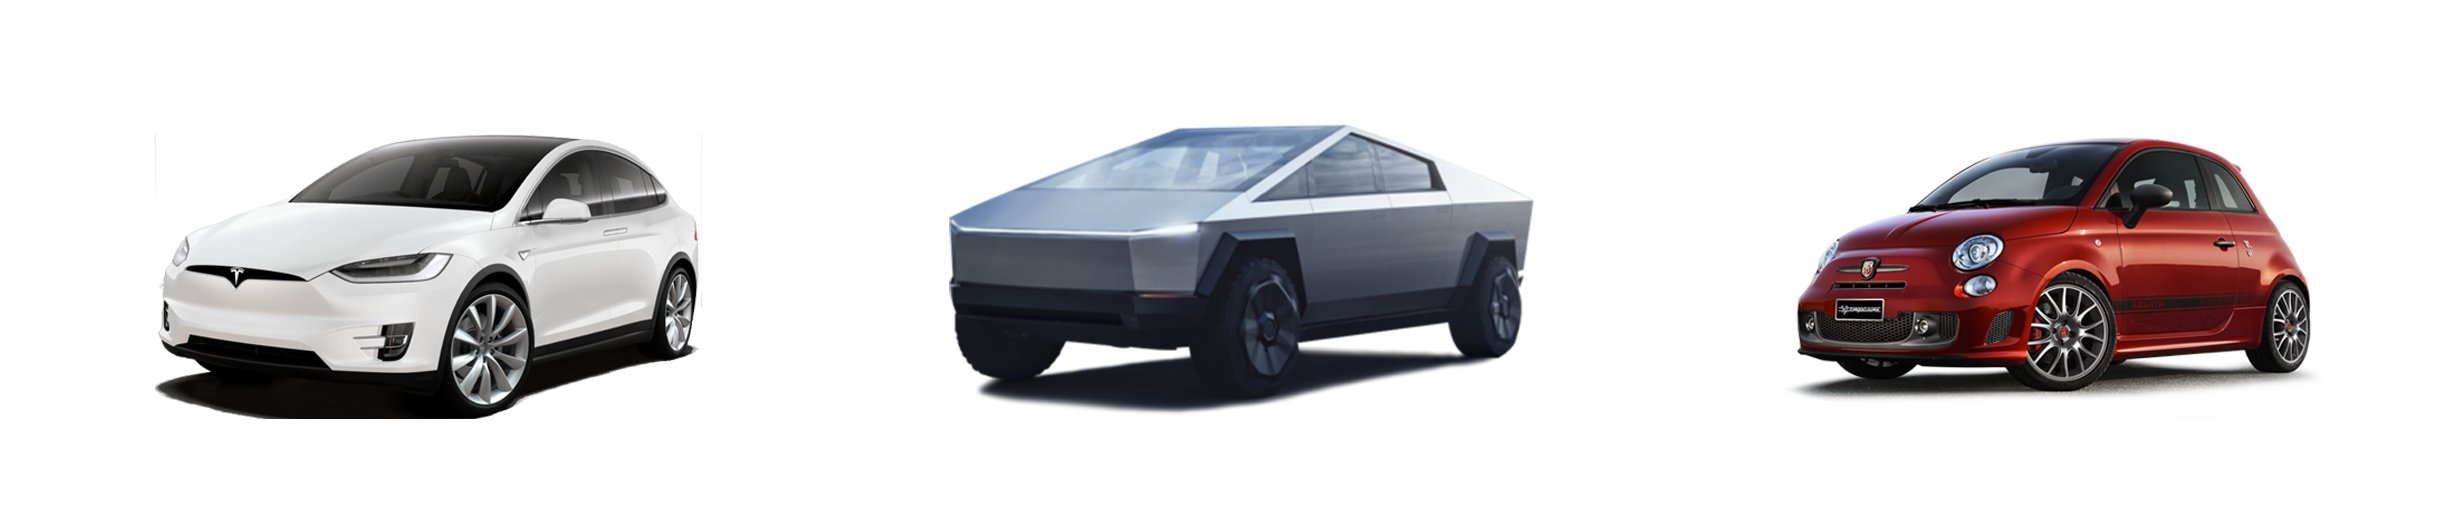
\includegraphics[width = 0.9\linewidth]{AUTO.png}
            \centering
            \caption{Esempio di veicoli con feature differenti ma appartenenti alla stessa categoria (automobile)}
            \label{auto}
        \end{figure}
        \item \emph{Condizioni dell'immagine}: Oltre al concetto temporale, i motivi che 
        portano ad una variabilità intra-calasse possono essere l'occlusione, 
        l'illuminazione, posa, punto di vista, ambiente circostante, condizioni 
        meteorologiche etc. Questi fattori influenzanti possono incidere 
        negativamente sull'aspetto di un oggetto. Ulteriori problematiche possono 
        riguardare l'aggiunta di artefatti di digitalizzazione, presenza del 
        rumore, bassa risoluzione e distorsioni varie (Fig. \ref{agenti atmosferici}).
        \begin{figure}
            \centering
            \hspace*{1.7cm}
            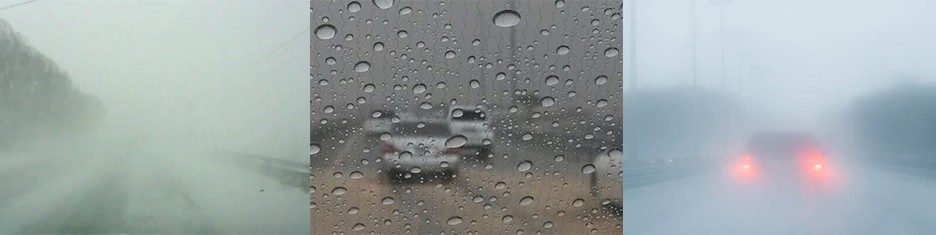
\includegraphics[width = 0.8\linewidth]{nebbia.png}
            \centering
            \caption{Esempio di immagini con scarsa visibilità e a basso contenuto informativo.}
            \label{agenti atmosferici}
        \end{figure}
    \end{enumerate}
    \item \emph{Numero di categorie}: il numero di classi può rilevarsi un problema quando 
    queste sono numerose. Un elevato numero di classi, oltre che ad aumentare 
    la probabilità di avere una bassa variabilità inter-calasse, richiede un alto 
    numero di etichette che a loro volta sono difficili da reperire. In questo caso 
    è favorita un'alta variabilità inter-classe (oggetti diversi appartenenti a classi 
    diverse). Ad oggi, l'utilizzo dell'esatto numero di esempi per addestrare un 
    modello è una domanda di ricerca ancora aperta;
    \item \emph{Efficienza}: attualmente non è possibile eseguire un modello complesso su 
    dispostivi sprovvisti di elevate risorse di calcolo. La ricerca è rivolta nell'ottimizzazione 
    di tali modelli affinché questi vengano eseguito anche su dispositivi mobili.
\end{itemize}

\subsubsection{Metriche di valutazione Object detection}
Le prestazioni di un modello vengono calcolate utilizzando alcune metriche, come 
per esempio i \emph{Frame Per Secondo (FPS)}, \emph{Precisione} e \emph{Recall}, ma la più usata è la 
\emph{mean Average Precision (mAP)}. La precisione misura la percentuale di previsioni 
corrette mentre il richiamo misura le previsioni corrette rispetto alla verità 
di base (\emph{ground truth}).
\begin{eqnarray}\label{precision}
    Precision & = & \frac{True \ Positive}{True \ Positive + False \ Positive} \nonumber \\
             & = & \frac{True \ Positive}{All \ Observations}
\end{eqnarray}
\begin{eqnarray}\label{recall}
    Recall & = & \frac{True \ Positive}{True \ Positive + False \ Negative} \nonumber \\
             & = & \frac{True \ Positive}{All \ Ground \ Truth}
\end{eqnarray}
Gli output standard di un rilevatore, su un'immagine di test $I$, al fine di 
identificare un oggetto $j$, sono:
\begin{itemize}
    \item $b_j$: \emph{Bounding-Box (BB)} disegnata sull'oggetto di interesse;
    \item $c_j$: categoria predetta;
    \item $p_j$: livello di confidenza che verrò comparato con una soglia $\beta$ per determinare 
    l'accettabilità o meno dell'etichetta della classe predetta. 
\end{itemize}
Una predizione $(b,c,p)$ è considerata come un vero positivo $(TP)$ se:
\begin{enumerate}
    \item La categoria predetta $c$ è uguale all'etichetta $c_g$ fornita nel ground truth;
    \item \emph{L'Intersection Over Union (IoU)} (\ref{iou}), è maggiore di una soglia $\epsilon$. L'IoU 
    rappresenta il rapporto tra l'area della bounding box predetta $b$ e l'area 
    della bounding box $b_g$ presente nel ground truth, dove $\cap$ e $\cup$ indicano 
    rispettivamente l'intersezione e l'unione delle varie aree.
    \begin{eqnarray}\label{iou}
        IoU(b,b_g) & = & \frac{area(b \cap b_g)}{area(b \cup b_g)} \nonumber \\
                 & = & \frac{Area \ of \ overlap}{Area \ of \ union}
    \end{eqnarray}
    Quando il modello prevederà una bounding box con un valore IoU maggiore 
    o uguale alla soglia,  tipicamente pari a 0.5, allora questo vuol dire che ci 
    sarà un'elevata sovrapposizione tra questa e una delle bounding box presenti 
    nel ground truth. D'altra parte, quando il valore di IoU è minore della 
    soglia, questo sintomo sarà ritenuto come una previsione errata da parte 
    del modello in quanto non c'è sovrapposizione fra le varie bounding box. 
    Questo comportamento fa si che la regione rilevata venga classificata come 
    un Falso Positivo \emph{(FP)}. Se invece il modello non riesce a rilevare un oggetto 
    presente nell'immagine, allora si parlerà di Falso Negativo $(FN)$.
    \begin{equation}\label{iou values}
        class(IoU) = \left\{
            \begin{array}{rl}
            TP & \mbox{if } IoU \geq \epsilon \\
            FP & \mbox{if } IoU < \epsilon \\
            FN & \mbox{if } IoU = \emptyset
            \end{array}
            \right.
    \end{equation}
\end{enumerate}
A questo punto, per poter calcolare l'Average Precision, consideriamo la $IoU$ come 
la nostra precisione \cite{rosebrock2017deep}. L'average precision, calcolata su una singola classe $i$, sarà 
quindi definita come:
\begin{equation}\label{average precision}
    AP_i = \frac{IoU}{L_i}
\end{equation}
Dove $L_i$ rappresenta il numero totale delle label appartenenti a una specifica classe 
$i$. La \emph{mean Average Precision (mAP)} sarà possibile calcolarla con la seguente formula:
\begin{equation}\label{mean average precision}
    mAP = \frac{1}{N}\sum_{i=1}^NAP_i
\end{equation}
dove N rappresenta il numero totali di classi e $AP_i$ rappresenta l'\emph{Average Precision} 
della classe $i$.

\subsection{Image Segmentation}
Nella Figura (\ref{segmentation}) è stato introdotto brevemente l'argomento della segmentazione 
delle immagini.  I recenti risultati, raggiunti nella segmentazione delle immagini, 
derivano dai progressi svolti nell'ottimizzazione delle \emph{Deep Convolutional Neural 
Networks (DCNN)}, in particolare dalle Convolutional Neural Networks (CNN). 
Nel 1989, sempre LeCun inventò \emph{LeNet-5} \cite{LeNet-5}, una rete neurale convoluzionale 
sviluppata per riconoscere i numeri scritti a mano. Grazie a questa, venne spianata 
la strada verso il continuo successo delle CNN nello svolgere vari compiti di visione 
artificiale di alto livello, oltre che a motivare i ricercatori ad esplorare le capacità 
di tali reti per problemi di classificazione pixel-wise, come la segmentazione delle 
immagini. La segmentazione di un'immagine è uno dei  compiti indispensabili 
nella visione artificiale in quanto è utile in diversi campi scientifici, come per 
esempio la guida autonoma, ambito medico, ambito biometrico, ambito militare, 
riconoscimento etc. Per poter svolgere questo complicato compito, a differenza 
della classificazione e dell'object detection, è necessario reperire delle informazioni 
spaziali di basso livello o a livello di pixel.
L'image segmentation si suddivide in due categorie:
\begin{enumerate}
    \item \emph{Semantic segmentation}
    \item \emph{Instance segmentation}
\end{enumerate}
Esiste un'ulteriore categoria, chiamata \emph{Panoptic Segmentation}, derivata dalla 
fusione dei risultati provenienti dalle due principali categorie. In questo elaborato 
verrà discussa solamente la tecnica di Semantic Segmentation. prima di introdurre 
la tecniche citata, è doveroso specificare che la segmentazione delle immagini è 
un argomento trattato anche nell'elaborazione dei video.

\subsubsection{Semantic Segmentation}
Il deep learning ha fortemente promosso la ricerca sulla segmentazione semantica. 
La comunità industriale sta facendo enormi sforzi nello sviluppo di sistemi avanzati 
in grado di effettuare una segmentazione semantica. Per esempio, una fotocamera, 
installata nei diffusi dispositivi mobili, è in grado di produrre un ritratto mediante 
l'effetto di profondità, comunemente chiamato effetto bokeh, incorporando la tecnica 
di segmentazione. Nella segmentazione semantica ogni pixel viene classificato 
in base alla classe di appartenenza dell'oggetto presente nell'immagine (es: strada, 
automobile, pedone, edificio etc.). In questo caso, i pixel dell'immagine aventi la 
stessa etichetta, condividono determinate caratteristiche come colore, intensità, 
consistenza etc. In altre parole, la segmentazione semantica tende a suddividere 
l'immagine in sottoinsiemi che si escludono a vicenda, in cui ogni sottoinsieme 
rappresenta una regione significativa dell'immagine originale. Rispetto alle altre 
tecniche, la tecnica di semantic segmentation ha esigenze più elevate in quanto 
non si limita solamente a classificare gli oggetti presenti (image classification) e a 
rilevarne la loro posizione (object detection) mediante delle bounding box, ma 
mira a partizionare ogni regione dell'oggetto (foreground) rispetto alla regione 
di sfondo (background). Per esempio, le auto presenti nella Figura (\ref{semantic segmentation}), vengono 
raggruppate come un unica porzione di pixel \cite{aurelien}.
\begin{figure}
    \centering
    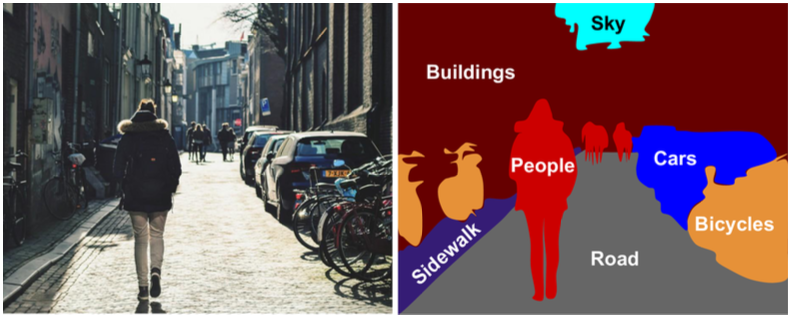
\includegraphics[width = 0.9\linewidth]{sem seg.png}
    \centering
    \caption{Esempio Semantic segmentation.}
    \label{semantic segmentation}
\end{figure}
Allo stato dell'arte esistono varie tipologie di architetture di reti neurali 
comunemente utilizzate per produrre delle segmentazioni semantiche \cite{semantic_segmentation_networks}:
\begin{enumerate}
    \item \emph{Fully convolutional networks (FCN)}
    \item \emph{Dilation/Atrous convolution}
    \item \emph{Top-Down/Bottom-up approach}
    \item \emph{Global Context}
    \item \emph{Receptive field enlargement and multi-scale context incorporation}
\end{enumerate}

\subsubsection{FULLY CONVOLUTIONAL NETWORKS}
Long et al. \cite{fcn} propose la pietra miliare Fully Convolutional Network (FCN), 
che diede un gran contributo all'incremento dell'accuratezza della segmentazione 
semantica. Lo studio si basò sull'utilizzo di svariati classificatori come: AlexNet \cite{alexnet}, 
VGGNet\cite{vggNet} e GoolgeNet \cite{googleNet}, tutte pre-addestrare con gli stessi dati. 
Ogni classificatore, come precedentemente spiegato in \ref{RNC}, ha lo scopo di prendere 
un'immagine in input e ridimensionarla tramite l'attraversamento dei layer 
convoluzionali, fino a giungere ai layer fully connected (FC). L'output prodotto 
sarà sotto forma di label predetta (Fig. \ref{CNN complete}). Per convertire questi modelli da 
classificatori a modelli FCN densi, bisogna sostituire i layer fully connected con 
layer convoluzionali di dimensione $1 \times 1 \times 21$, dove 21 rappresenta il numero delle 
classi esistenti in PASCAL VOC (20), più la classe di background. Tramite una 
procedura di \emph{Upsampling}, viene effettuata un'operazione di \emph{deconvoluzione}, spesso 
chiamata \emph{convoluzione trasposta}, utile a restituire in ouput l'immagine di partenza 
ricostruita. Esistono varie tipologie di upsampling, fra queste abbiamo:
\begin{enumerate}
    \item \emph{Nearest-Neighboor}: Copia il valore del pixel più vicino;
    \item \emph{Up-Sampling Bilineare}: calcola il valore dei pixel attraverso l'interpolazione lineare e l'uso dei pixel adiacenti;
    \item \emph{Up-sampling Bicubico}: Calcola il valore dei pixel attraverso l'interpolazione polinomiale. Questa operazione ha un alto tasso computazionale ma allo stesso tempo produce risultati migliori rispetto alle sue concorrenti. 
\end{enumerate}
Quando si sarà giunti a un layer di pooling pari alla dimensione di $1 \times 1$, allora 
si potrà attuare l'upsampling per poter ricostruire l'immagine di partenza (Fig. \ref{FCN}). 
\begin{figure}
    \centering
    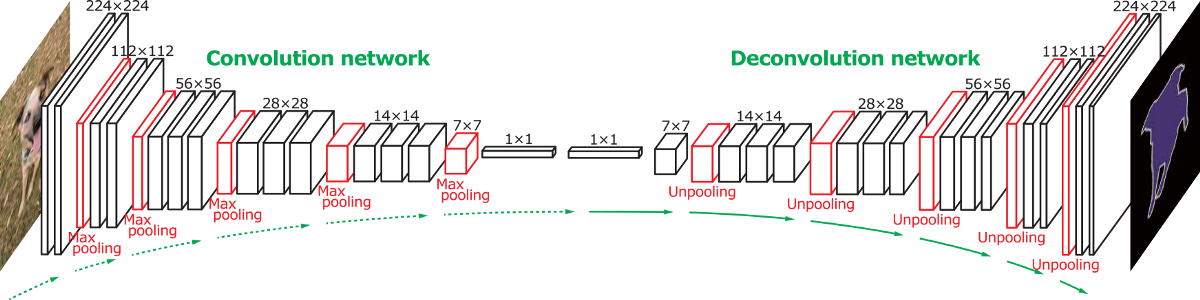
\includegraphics[width = \linewidth]{FCN.png}
    \centering
    \caption{Esempio di architettura Fully Convolutional Network}
    \label{FCN}
\end{figure}
Tale architettura è composta da un \emph{Encoder} e da un \emph{Decoder}.
\begin{itemize}
    \item \emph{Encoder}: sezione dell'architettura adibita all'estrazione del contesto dell'immagine. 
    La sua struttura è composta da livelli di convoluzione e di max 
    pooling, come una comune CNN, che riducono (down-sample) l'immagine 
    in ingresso; 
    \item \emph{Decoder}: sezione dell'architettura adibita alla localizzazione degli elementi 
    presenti nell'immagine attraverso l'utilizzo di convoluzioni trasposte. Il compito 
    di un decoder è quello di amplificare le feature map tramite operazioni 
    di deconvoluzione utili a ricostruire l'immagine di ingresso includendone i 
    suoi artefatti.
\end{itemize}
Esitono diverse reti FCN che adottano questa tipologia di architettura (es: \emph{Autoencoder}). 
Per quanto riguarda le operazioni 
svolte, un confronto tra l'operazione di Pooling (downsampling) e di Unpooling 
(upsampling), o di convoluzione e deconvoluzione, sono mostrate nella 
Figura \ref{deconvolution}.
\begin{figure}
    \centering
    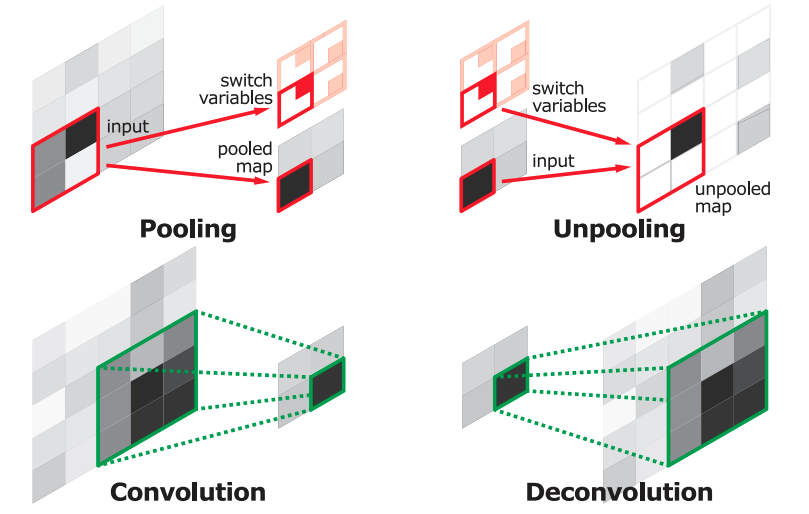
\includegraphics[width = 0.7\linewidth]{deconvolution.png}
    \centering
    \caption{Esempio di Deconvoluzione e di Unpooling (Upsampling).}
    \label{deconvolution}
\end{figure}
In base al numero di layer convoluzionali presenti, esistono diverse architetture 
di Fully Convolutional Networks. Una fra queste, la \emph{FCN-32}, è composta da 
un encoder che ha il compito di ridurre l'immagine iniziale di 32 volte e da un 
decoder che svolgerà il processo inverso di ricostruzione. Avendo pochi dati a 
disposizione, la rete farà fatica a ricostruire un output simile a all'input, questo si 
verifica a causa della perdita delle informazione significative nel processo svolto 
dall'encoder. Per avere una rappresentazione più fedele dell'immagine in output, 
vengono in auto altre due tipologie di architetture: \emph{FCN-16} e \emph{FCN-8}.
\begin{figure}
    \centering
    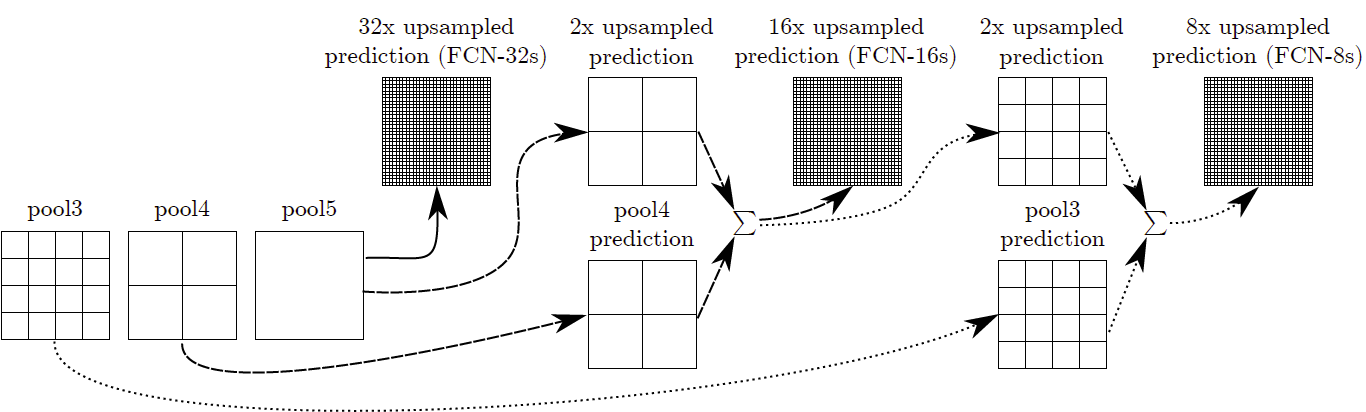
\includegraphics[width = \linewidth]{FCN-32.png}
    \centering
    \caption{Esempio derivazione delle varie architetture FCN.}
    \label{FCN-models}
\end{figure}
Quest'ultime utilizzano una strategia intelligente per poter ricostruire l'immagine. 
Per giungere a un buon risultato, oltre che a fare riferimento alla sola feature 
map, utilizzano i livelli di pooling precedenti nella quale ci sono maggiori informazioni. 
Per giungere ad un'architettura FCN-8, bisognerà svolgere un processo 
iterativo che va ad effettuare una somma di ogni singolo elemento (element-wise) 
tra l'upsampling del pooling layer $n$ con il pooling layer $n-1$ (Fig. (\ref{FCN-models})). La ricostruzione 
risultante sarà quella più fedele al ground truth. Questa architettura 
ha permesso di convertire i modelli precedenti in \emph{FCN-AlexNet}, \emph{FCN-VGG16} e 
\emph{FCN-GoogleNet}.

\subsubsection{DILATATION/ATROUS CONVOLUTION}
\subsubsection{DilatedNet}
Per rimediare alla bassa qualità prodotta in output da una comune rete CNN, Yu 
e Koltun introdussero un versione modificata chiamata {\bfseries{Convoluzione Dilatata}} 
o {\bfseries{DilatedNet}} \cite{DilatedNet}. Questo modello consentiva di estrarre le informazioni che 
consentivano una migliore segmentazione che non comportasse a sua volta alla 
perdita di dati rilevanti. L'idea della Convoluzione dilatata, chiamata anche 
\emph{Convoluzione Dilatata}, o \emph{"Atrous Algorithm"} (il termine deriva dal francese \emph{à trous} che significa "buco" o "foro"),  deriva dalla decomposizione wavelet. A differenza del 
tradizionale operatore di convoluzione, la convoluzione dilatata introduce un tasso 
di dilatazione \emph{(dilated rate)} $l$, utile a saltare alcuni punti, presenti nel 
campo ricettivo, durante la convoluzione. La formula matematica per il calcolo della 
convoluzione dilatata è la seguente:
\begin{equation}
    (F*_lk)(p) = \sum_{s+lt=p}F(s)k(t)
\end{equation}
dove:
\begin{equation}\label{dilated rate}
    Conv(l) = \left\{
        \begin{array}{rl}
        Standard & \mbox{if } l = 1\\
        Dilated & \mbox{if } l > 1
        \end{array}
        \right.
\end{equation}
Con un dilated rate pari a 2, otterremmo la seguente convoluzione dilatata (Fig. (\ref{dilated})):
\begin{figure}
    \centering
    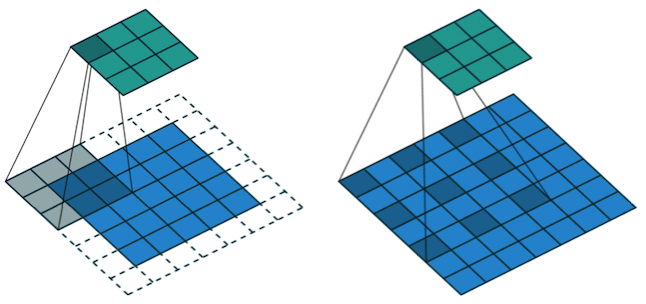
\includegraphics[width = 0.8\linewidth]{dilated.png}
    \centering
    \caption{Esempio di convoluzione standard ($l=1$)(Sinistra) e di Convoluzione Dilatata ($l=2$) (Destra).}
    \label{dilated}
\end{figure}
Maggiore sarà il valore del tasso di dilatazione, maggiore sarà il campo ricettivo 
e minore saranno i calcoli da svolgere. 

\subsubsection{DeepLab}\label{DeepL}
DeepLab è un modello utilizzato allo stato dell'arte per la segmentazione semantica 
progettato da Google. Per la costruzione della rete sono state affrontate due 
problematiche: il down-sampling e l'invarianza spaziale. Il primo problema, legato 
alla riduzione della risoluzione delle feature, è stato risolto grazie all'applicazione 
dell'algoritmo soprannominato “atrous”. Ogni encoder è composto dalla combinazione 
di layer di pooling che riducono la risoluzione spaziale delle feature map. 
Per poter ricostruire le informazioni perse, si può utilizzare la deconvoluzione. 
Quest'ultima richiede però un quantitativo importante di memoria e di tempo. 
L'algoritmo offre un metodo alternativo alla deconvoluzione. Il suo scopo 
è quello di applicare una convoluzione che permetta di allargare efficacemente il 
campo visivo dei filtri senza aumentare il numero di parametri preservando la 
quantità di computazione richiesta. La tecnica della convoluzione atrosa può essere 
vista come come un espediente della tecnica di upsampling. Per poter risolvere il 
secondo problema, legato alla precisione ridotta a causa dell'invarianza spaziale, 
questa tipologia di rete, al fine di catturare dettagli più fini, applica un \emph{Conditional 
Random Field (CRF)} completamente connesso. Questa classe di modelli 
discriminanti utilizzano le informazioni contestuali delle label per effettuare delle 
buone previsioni. Restando ad un discorso più ad alto livello, le potenzialità del 
CRF riguardano l'utilizzo di termini leviganti (\emph{smoothness}) utili a massimizzare la 
relazione tra le etichette di pixel simili che esaltano il foreground dal background. 
Questi termini permetto quindi di avere una mappa di segmentazione migliore 
anche dopo aver applicato poche volte, in maniera iterativa, l'algoritmo del CRF. 
L'architettura generale di un modello DeepLab (Fig. (\ref{CRF})) consiste nel prendere in input 
un'immagine e di elaborarla da una comune DCNN in cui ci sono degli strati 
atrosi, per poter generare una prima Score map su cui verrà fatto l'upsampling 
con un'interpolazione bilineare. Dopo aver estratto un'immagine avente le stesse
dimensioni dell'immagine di partenza, verrà applicato il CRF.
\begin{figure}
    \centering
    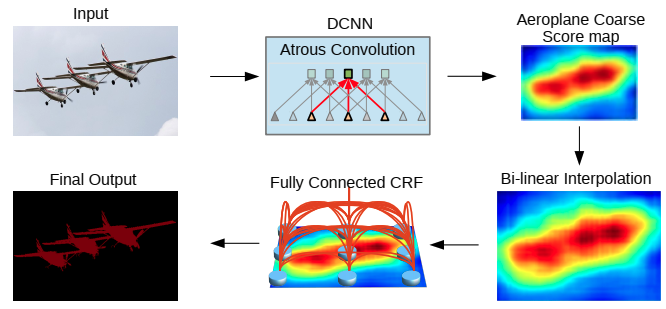
\includegraphics[width = \linewidth]{CRF.png}
    \centering
    \caption{Esempio architettura DeepLab.}
    \label{CRF}
\end{figure}

\subsubsection{TOP-DOWN/BOTTOM-UP APPROACH}
\subsubsection{U-Net}
La rete U-Net \cite{unet} è una rete di segmentazione semantica, con una architettura a forma 
di U (Fig. (\ref{unet})) composta anch'essa da un encoder, o percorso di contrazione, e 
un decoder, o percorso di espansione.
\begin{figure}
    \centering
    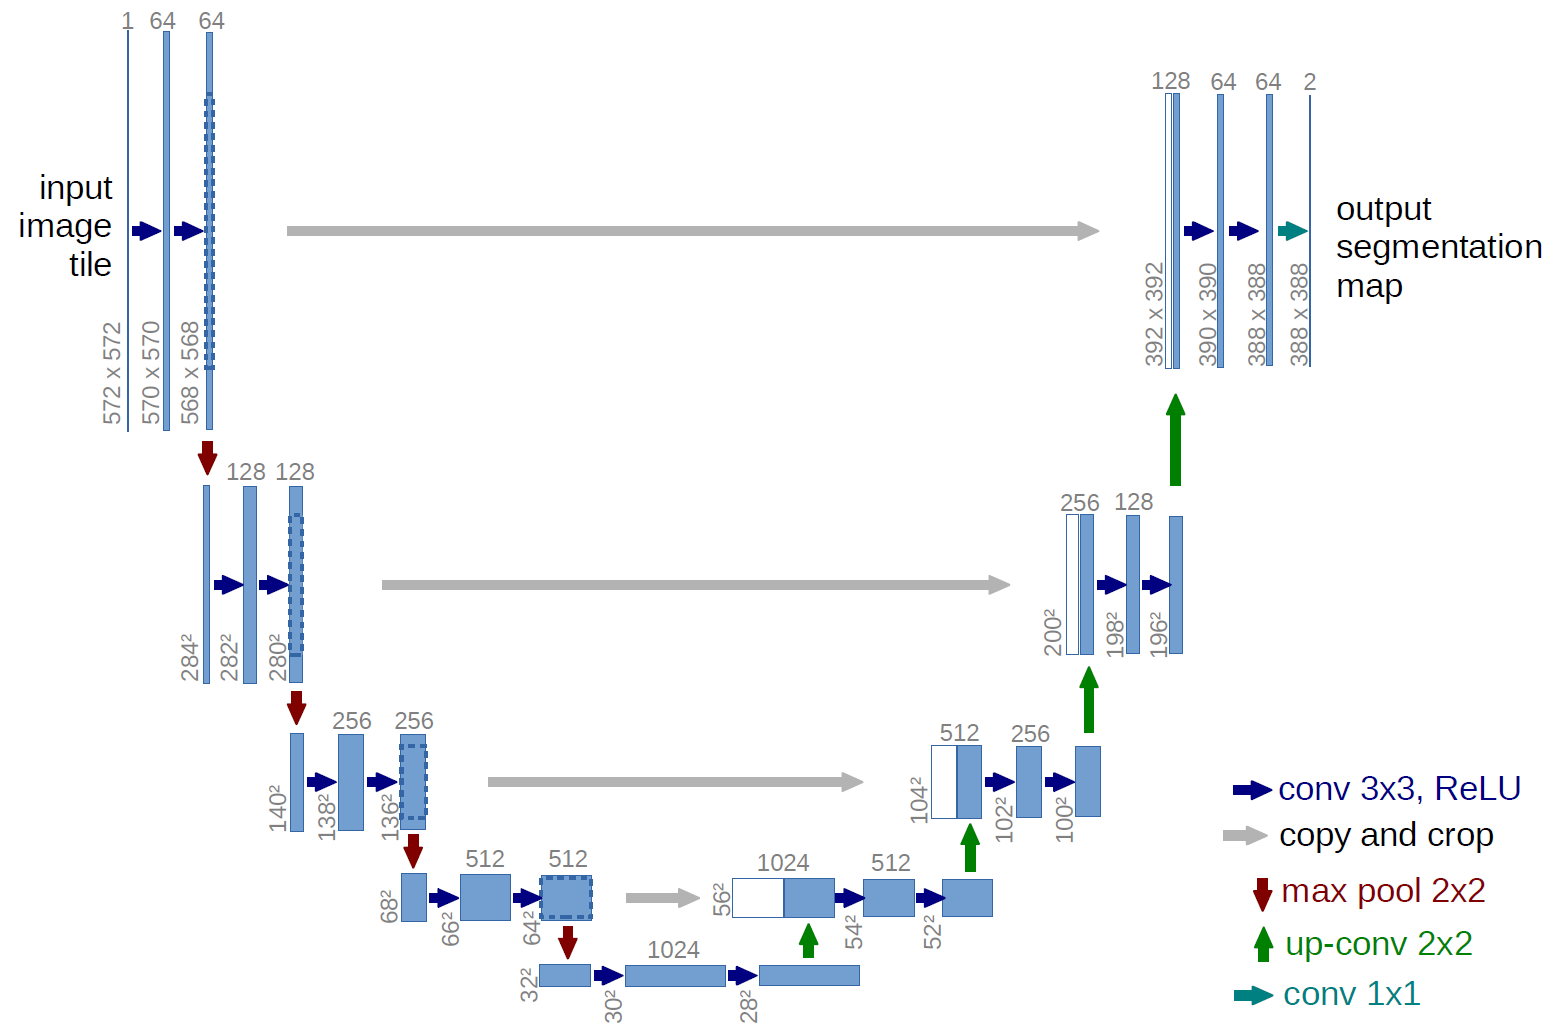
\includegraphics[width = \linewidth]{Unet.png}
    \centering
    \caption{Esempio architettura rete U-Net.}
    \label{unet}
\end{figure}
Nell'immagine, ogni riquadro blu rappresenta una feature map multicanale. Il 
numero dei canali (specificati sopra ogni riquadro) e le dimensioni (specificate in 
basso a sinistra di ogni riquadro), variano in base alla profondità della rete. I 
riquadri bianchi, presenti nello strato di decoder, stanno a rappresentare le feature 
map copiate dallo strato dell'encoder. Fra i vari layer esistenti in entrambe le 
parti, esistono delle connessioni, chiamate \emph{Shortcut connection}, capaci di creare 
un collegamento utile a trasferire le informazioni estratte dall'encoder verso il 
decoder. Questi collegamenti sono utili a velocizzare il processo di up-sampling e 
migliorare nel contempo il risultato finale. La sezione dell'encoder è formata da 
due convoluzioni $3 \times 3$ consecutive, seguite dalla funzione di attivazione ReLU e 
da un'operazione di max-pooling avente una finestra di dimensioni $2 \times 2$ con 
passo 2. Dalla parte del decoder invece abbiamo l'operazione di up-sampling delle 
feature map seguita da una deconvoluzione $2 \times 2$. La mappa delle caratteristiche 
risultati viene concatenata con la mappa delle caratteristiche ritagliata estratta 
dall'encoder. Successivamente, vengono applicate due operazione di convoluzioni 
consecutive aventi finestra di dimensione pari a $3 \times 3$.

\subsubsection{SegNet}
Così come i modelli già visti, anche SegNet ha un'architettura composta da un 
encoder e un decoder. La parte adibita all'encoder utilizza 13 layer convoluzionali, 
mentre la parte destinata al decoder contiene anch'essa 13 layer per la deconvoluzione. 
In ogni layer della sezione encoder, viene utilizzato un banco di filtri 
per produrre le feature map. Per poter ridurre lo spostamento della covarianza 
interna, problema legato all'input che porta la rete a non essere abbastanza 
efficiente e/o ad avere una scarsa generalizzazione, viene utilizzata una tecnica 
nota come batch normalization \cite{batchNorm} seguita da una funzione attivazione ReLU. Su 
ogni feature map viene applicato un max-pooling con una finestra di dimensioni 
$2\times 2$ e passo 2. Come già noto, un alto numero di operazioni si sub-sampling 
comporta una maggiore precisione di classificazione, ma allo stesso tempo provoca 
una riduzione di ogni feature map che, tradotto in altri termini, causa la perdita 
dei dati. La riduzione del numero di dati determina la creazione di bordi sfocati 
il quale rappresenta un problematica centrale per un'operazione di segmentazione. 
Per risolvere il problema della perdita dei dati, SegNet effettua solo una memorizzazione 
degli indici di pooling per ciascuna feature map prodotta dall'encoder. 
Tali indici saranno utili al decoder per effettuare l'operazione di upsampling 
al fine di costruire delle feature map ad alta risoluzione che avessero l'obiettivo di 
produrre un'immagine in output avente le stesse dimensioni di quella in input. 
Per giungere al risultato finale, anche il decoder utilizza un banco di filtri, a loro 
volta aggiornabili in fase di addestramento, per poter effettuare la deconvoluzione. 
La feature map prodotta da un decoder verrà inserità in un classificatore softmax 
multi-classe addestrabile che effettuerà l'etichettatura di ogni singolo pixel (Fig. (\ref{segnet})).
\begin{figure}
    \centering
    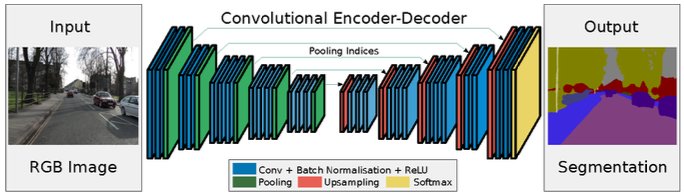
\includegraphics[width = \linewidth]{segnet.png}
    \centering
    \caption{Esempio architettura SegNet.}
    \label{segnet}
\end{figure}

\subsubsection{GLOBAL CONTEXT}
\subsubsection{ParseNet}
Un significativo miglioramento delle reti FCN ebbe inizio con l'introduzione della 
rete ParseNet \cite{parsenet}. Codesta, a differenza delle reti FCN, utilizza le informazioni 
inerenti le feauture globali, o contesto globale, per poter produrre in output una 
buona segmentazione dell'immagine (Fig. (\ref{global context})).
\begin{figure}
    \centering
    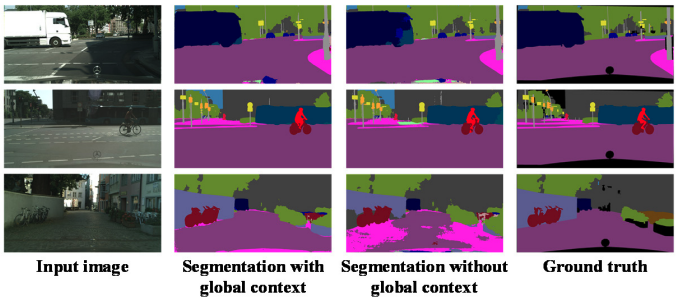
\includegraphics[width = \linewidth]{gloabal context.png}
    \centering
    \caption{Esempio di applicazione del contesto globale alla segmentazione.}
    \label{global context}
\end{figure}
Le feature globali sono utili per poter rappresentare un oggetto nella sua 
totalità. Per poter ricavare queste informazioni, vengono utilizzate delle feature 
map sulla quale viene eseguito il pooling mediante una media globale. Dopo aver 
effettuato il pooling, viene eseguita l'operazione inversa (\emph{un-pooling}) per poter 
riportare l'immagine alle sue dimensioni di partenza. Successivamente, le feature 
map di partenza e quelle ricavate vengono combinate per effettuare una previsione 
sul punteggio di classificazione finale. Ogni feature map appartiene a un layer 
diverso, pertanto la combinazione di queste sarà formata da feature map diverse 
in termini di scala e di norma. Affinché tutto funzioni, vengono applicate due 
normalizzazioni L2 (\ref{L2}), una dopo il pooling globale e l'altra dopo la feature 
map di partenza estratta contemporaneamente dalla FCN. 
\begin{equation}\label{L2}
    \norm{x}_2 = \left(\sum_{i=1}^d \abs{x_i}^2 \right)^\frac{1}{2}
\end{equation}
Dove $x$ rappresenta l'input e $d$ rappresenta la sua dimensionalità. Nel percorso 
inferiore, viene eseguita una normalizzazione L2, a ciasun livello di convoluzione, 
per ciascun canale. Nel percorso superiore invece, viene effettuato un pooling 
medio delle feature map in ogni specifico livello di convoluzione. Dopo aver 
ottenuto le feature globali, viene effettuata una normalizzazione L2. L'unpooling 
è utile a poter far combaciare le dimensioni dei vettori superiori con i vettori 
inferiori, in modo che questi possano essere concatenati. La figura (\ref{parsenet}) riassume 
i passaggi precedenti.
\begin{figure}
    \centering
    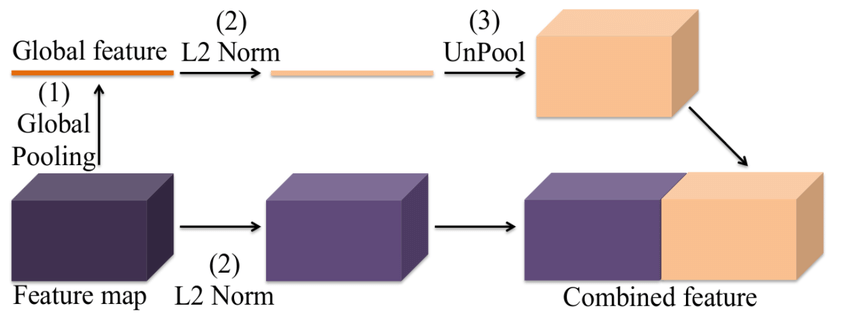
\includegraphics[width = 0.8\linewidth]{parsenet.png}
    \centering
    \caption{Modulo ParseNet.}
    \label{parsenet}
\end{figure}

\subsubsection{GCN}
La segmentazione semantica basa il suo principio di funzionamento su due aspetti: 
classificazione e localizzazione. Quest'ultimi sono ritenuti come due concetti 
di natura opposta in quanto, una piccola trasformazione dell'input, come ad 
esempio una traslazioni o rotazioni, rende la classificazione invariante mentre, allo 
stesso tempo, la localizzazione potrebbe risentirne negativamente, pertanto risulta 
essere più sensitiva rispetto alla classificazione. Per sopperire alle problematiche 
delle trasformazioni su entrambe le tecniche, venne introdotto il modello \emph{Global 
Convolutional Network (GCN)} \cite{gcn}. La rete è basata sui seguenti due principi:
\begin{enumerate}
    \item Dal punto di vista della \emph{localizzazione}, la struttura del modello dev'essere 
    completamente convolutiva per poter mantenere le informazioni utili alla 
    localizzazione degli oggetti in quanto, se la struttura fosse stata a livelli 
    completamente connessi (fully-connected layers), o pooling globali, questi 
    scarterebbero tutte le informazioni spaziali;
    \item Dal punto di vista della \emph{classificazione}, devono essere utilizzati dei kernel 
    di grandi dimensioni, circa $15\times 15$, al fine di consentire la realizzazione di 
    connessioni dense tra le feature map e le classificazioni pixel-wise. Questi 
    filtri consentono di effettuare delle convoluzioni globali che rendono la rete 
    invariante alle trasformazioni.
\end{enumerate}
Per poter migliorare il contorno della segmentazione, viene utilizzata il blocco 
\emph{Boundary Refinement (BR)} dopo l'applicazione del modulo GCN e durante 
il processo di deconvoluzione.
\begin{figure}
    \centering
    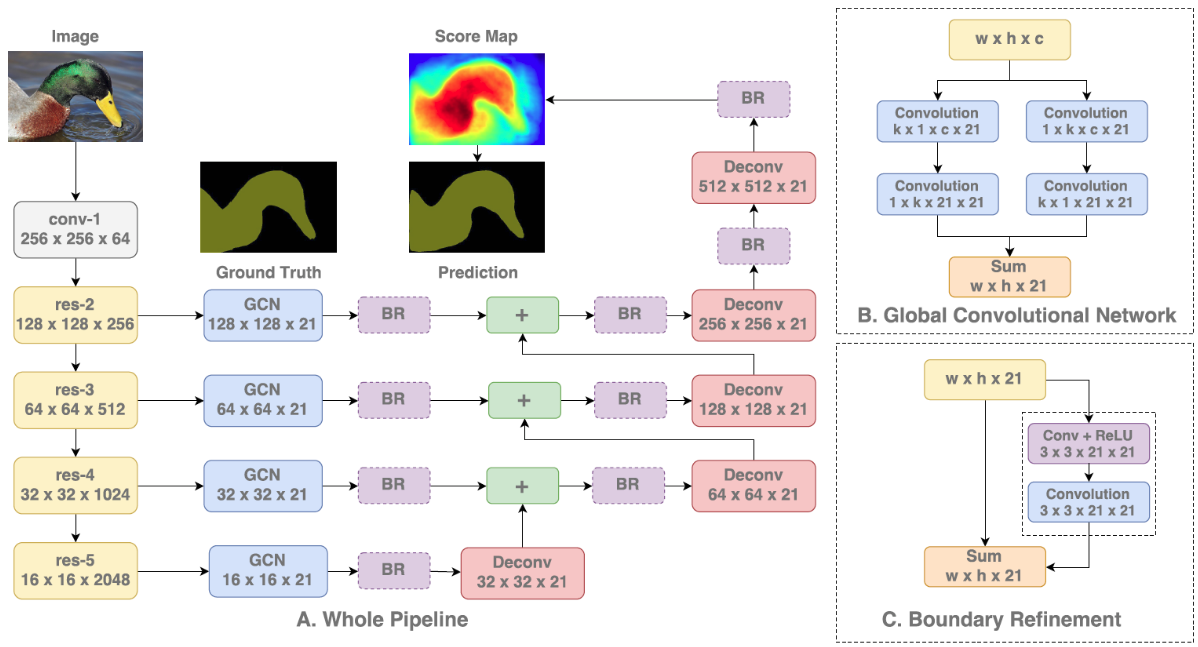
\includegraphics[width = \linewidth]{GCN.png}
    \centering
    \caption{Architettura modello GCN.}
    \label{gcn}
\end{figure}
Come visto in Figura (\ref{gcn}), ResNet è la rete che viene utilizzata come 
backbone (spina dorsale), pre-addestrata con le immagini contenute nel dataset 
ImageNet. Sulle mappe dei punteggi di bassa risoluzione viene effettuata un'operazione 
di upsampling con un layer di deconvoluzione. Le mappe ottenute dalla 
deconvoluzione verranno aggiunte con quelle più alte per poter generare nuove 
mappe dei punteggi utili alla segmentazione finale.

\subsubsection{RECEPTIVE FIELD ENLARGEMENT AND MULTI-SCALE CONTEXT INCORPORATION}
\subsubsection{DeepLabv2 e DeepLabv3}
La prima versione del modello DeepLab ha subito delle modifiche che hanno 
portato a dei miglioramenti in termini di performance. Gli stessi autori di 
DeepLab introdussero altre versioni del loro modello, in particolare introdussero 
DeepLabv2 \cite{deeplabv2} e DeepLabv3 \cite{deeplabv3}. La prima, rispetto alla prima versione, utilizza 
una tecnologia aggiuntiva chiamata \emph{Atrous Spatial Pyramid Pooling (ASPP)}.  
Quest'ultima ha il compito di aggregare diverse feature multi-scala per una 
migliore localizzazione. Per ogni tasso di dilatazione $l$ differente, la tecnica 
effettua una convoluzione dilatata ad ogni feature map di input che unirà con le 
restanti (Fig. (\ref{aspp})).
\begin{figure}
    \centering
    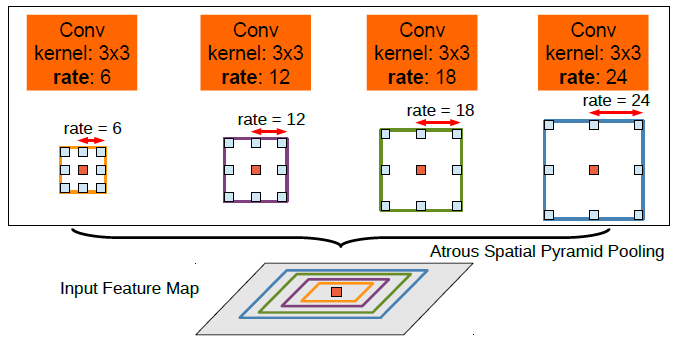
\includegraphics[width = 0.9\linewidth]{aspp.png}
    \centering
    \caption{Atrous Spatial Pooling Pyramid.}
    \label{aspp}
\end{figure}
Oltre a questa, l'architettura di DeepLabv2 utilizza non solo VGGNet come 
backbone , ma utilizza anche ResNet. Per quanto riguarda DeepLabv3, questo 
modello venne introdotto per poter catturare i bordi degli oggetti mediante il 
recupero delle informazioni spaziali. Per ottenere quanto detto, DeepLabv3 incorpora 
un encoder e un decoder con una convoluzione dilatata separata. L'encoder 
e il decoder sono utili per poter ricavare i contorni degli oggetti nitidi mentre 
la convoluzione dilatata viene applicata in profondità per aumentare l'efficienza 
computazionale. Per ottenere ciò viene fattorizzata una convoluzione standard in 
una \emph{convoluzione depth-wise}, seguita da una \emph{convoluzione point-wise} (convoluzione 
con kernel di dimensione 1x1). Una convoluzione di tipo depth-wise ha il compito 
di eseguire una convoluzione spaziale in maniera indipendente su ciascun canale, 
mentre una convoluzione point-wise effettua una combinazione delle uscite della 
convoluzione depth-wise su tutti i canali contemporaneamente (Fig. (\ref{depth and point})). È bene ricordare 
che il kernel utilizzato per la convoluzione depth-wise ha un numero di canali pari 
a quello presenti nell'immagine di input.
\begin{figure}
    \centering
    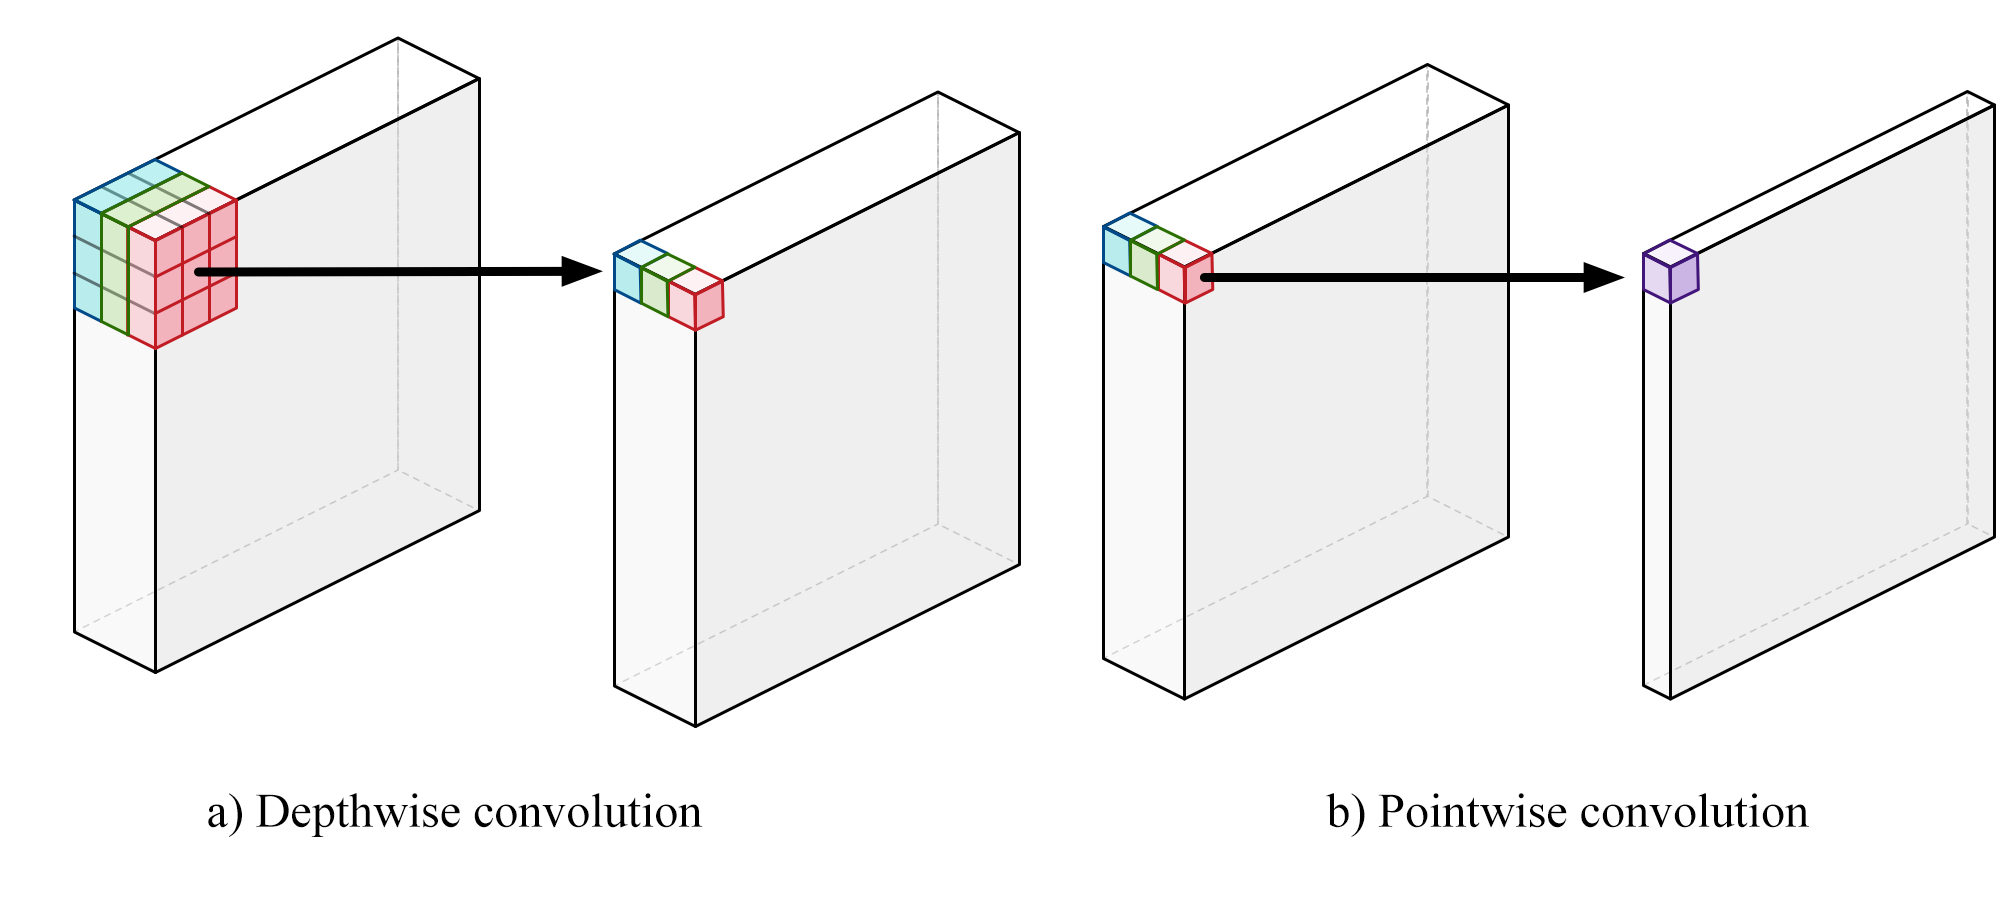
\includegraphics[width = \linewidth]{depth and point.png}
    \centering
    \caption{Differenza tra convoluzione depth-wise (a) e convoluzione point-wise (b).}
    \label{depth and point}
\end{figure}

\subsubsection{PSPNet}
L'ultima tipologia di rete mostrata è chiamata \emph{Pyramid Scene Parsing Network 
(PSPNet)} \cite{pspnet}. All'interno di questa rete viene utilizzato il modulo \emph{Pyramid 
Pooling} che ha il compito di effettuare un pooling, su ogni feature map iniziale, 
utilizzando quattro differenti scale corrispondenti a quattro differenti livelli 
piramidali, corrispettivamente di dimensione $1\times 1$, $2\times 2$, $3\times 3$ e $6\times 6$, 
come mostrato in Figura (\ref{pspnet}).
\begin{figure}
    \centering
    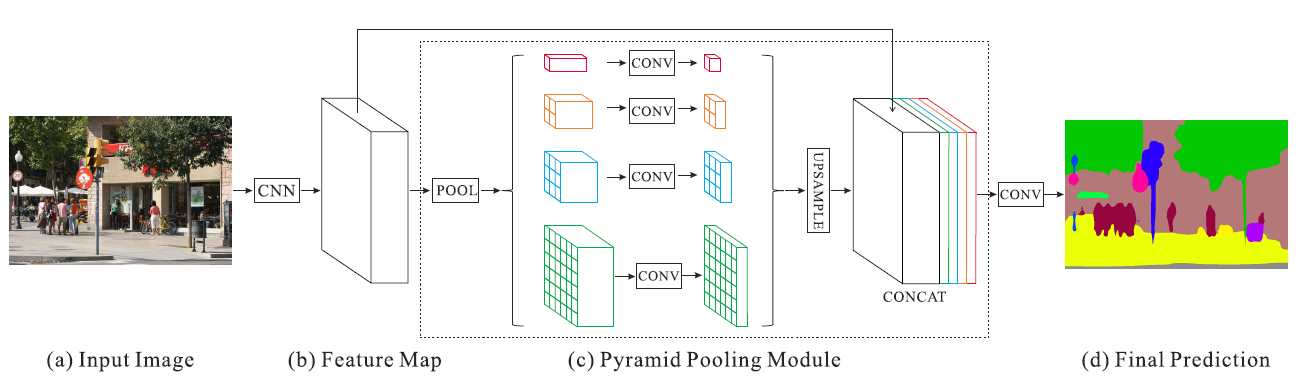
\includegraphics[width = \linewidth]{pspnet.png}
    \centering
    \caption{Architettura PSPNet.}
    \label{pspnet}
\end{figure}
Anche in questa rete viene utilizzata ResNet per poter estrarre le feature. La 
convoluzione dilatata è come quella eseguita in DeepLab. Le dimensioni della 
feature map è ridotta di circa $1/N$ rispetto all'immagine di input, dove $N$ sta ad 
indicare i livelli della piramide. Nella figura (\ref{pspnet}), il numero di livelli piramidali 
è pari a 4, pertanto $N=4$, che a sua volta si traduce in un a riduzione pari a 
$1/4$ dell'immagine di partenza. Per ridurre le dimensioni dei layer di pooling, 
viene effettuata una convoluzione di dimensioni $1\times 1$. Gli output prodotti dalle 
varie convoluzioni sono sottoposti a processo di upsampling e concatenati con 
le feature map iniziali per poter combinare le informazioni contestuali locali e 
globali. Infine, l'intera concatenazione sarà convoluta per poter generare una 
predizione pixel-wise utile a realizzare la segmentazione semantica finale.

\subsubsection{Metriche di valutazione Image Segmentation}
Così come per l'Object detection, anche l'Image Saegmentation dispone di tecniche 
per poter valutare la segmentazione effettuata da un modello. Immaginiamo di 
avere un numero $k$ di classi esistenti e che a questo venga sommata un'ulteriore 
classe di background, per un totale di $k+1$ classi. Denotiamo inoltre con $Y$ il 
numero di pixel totali dell'immagine da segmentare. Secondo \cite{metric_semantic_seg}, immaginiamo di dover segmentare i pixel di una classe $i$, definiamo tre 
tipologie di valori associati a $Y$:
\begin{enumerate}
    \item $Y_{ii}$: denotano il numero di pixel predetti appartenenti alla classe $i$ ed 
    effettivamente corrispondenti alla classe $i$ (\emph{True Positive (TP)});
    \item $Y_{ij}$: denotano il numero di pixel predetti appartenenti alla classe $j$ e quindi 
    non corrispondenti alla classe $i$ (\emph{False Positive (FP)});
    \item $Y_{ji}$: denotano il numero di pixel predetti appartenenti alla classe $i$ ma 
    corrispondenti alla classe $j$ (\emph{False Negative (FN)});
\end{enumerate}
Di seguito vengono elencate le cinque più famose tecniche per poter valutare 
l'accuratezza della segmentazione semantica:
\begin{itemize}
    \item {\bfseries{\emph{Pixel Accuracy (PA)}}}: rappresenta il rapporto tra il numero di pixel 
    correttamente segmentati e il numero totale di pixel. In altre parole, tale 
    rapporto può essere rappresentato come $TP/(TP+FN)$. La formula per 
    ricavare la PA è la seguente:
    \begin{equation}
        PA = \frac{\sum_{i=0}^kY_{ii}}{\sum_{i=0}^k\sum_{j=0}^kY_{ij}}
    \end{equation}

    \item {\bfseries{\emph{Mean Pixel Accuracy (MPA)}}}: rappresenta un'estensione della Pixel 
    Accuracy. Ha lo scopo di calcolare l'accuratezza media dei pixel per ogni 
    classe. La MAP può essere ottenuta dalla seguente formula:
    \begin{equation}
        MPA = \frac{1}{k+1}\sum_{i=0}^k\frac{Y_{ii}}{\sum_{j=0}^kY_{ij}}
    \end{equation}

    \item {\bfseries{\emph{Intersection Over Union (IoU)}}}: seppur incontrata nella sezione inerente 
    l'object detection (\ref{OBJD}), l'IoU per la semantic segmentation non rappresenta 
    più il rapporto tra la sovrapposizione di una bounding box predetta con 
    la bounding box del ground truth, ma questa volta sta a rappresentare la 
    percentuale di sovrapposizione tra la regione predetta e la regione target 
    appartenente al ground truth (\ref{predSegIoU}). In altre parole, l'IoU può essere rappresentata 
    come $TP/(TP+FP+FN)$, che da un punto di vista matematica è espresso come:
    \begin{equation}\label{predSegIoU}
        IoU = \frac{target\cap prediction}{target\cup prediction}
    \end{equation}
    \begin{equation}
        IoU = \frac{\sum_{i=0}^kY_{ii}}{\sum_{i=0}^k\sum_{j=0}^kY_{ij}+\sum_{i=0}^k\sum_{j=0}^kY_{ji}-\sum_{i=0}^kY_{ii}}
    \end{equation}

    \item {\bfseries{\emph{Mean Intersection over Union (MIoU)}}}: l'IoU viene calcolata separatamente 
    per ogni classe. La MIoU rappresenta la media di tutte le IoU, e 
    quindi su tutte le classi, utile a fornire un punteggio globale del modello che 
    può essere calcolato con la seguente formula:
    \begin{equation}
        MIoU = \frac{1}{k+1}\sum_{i=0}^k\frac{Y_{ii}}{\sum_{j=0}^kY_{ij}+\sum_{j=0}^kY_{ji}-Y_{ii}}
    \end{equation}

    \item {\bfseries{\emph{Frequency-Weighted Intersection over Union (FWIoU)}}}: questa metrica 
    rappresenta un'estensione della MIoU. La FWIoU utilizza la frequenza 
    di occorrenza per poter regolare l'importanza di ciascuna classe. La formula 
    per il suo calcolo è la seguente:
    \begin{equation}
        FWIoU = \frac{1}{\sum_{i=0}^k\sum_{j=0}^kp_{ij}}\sum_{i=0}^k\frac{\sum_{j=0}^kY_{ij}Y_{ii}}{\sum_{j=0}^kY_{ij}+\sum_{j=0}^kY_{ji}-Y_{ii}}
    \end{equation}
\end{itemize}
Nella segmentazione semantica è importante valutare il modello nella sua efficienza 
per applicazioni real-time. Per calcolare la complessità di un modello, possono 
essere tenute in considerazione due metriche come il numero dei parametri e le 
operazioni in virgola mobile (\emph{Floating Point Operations - FLOPs}). Maggiori 
sono questi due valori e minori saranno le prestazioni del modello. Entrambe 
le metriche sono indipendenti dall'ambiente. Per quanto riguarda la velocità di 
implementazione, possono essere utilizzate due metriche: \emph{Runtime} e, come per 
la tecnica di Object detection, i \emph{Frame al secondo (Frame Per Second - FPS)}. 
Quest'ultime due metriche, a differenza delle precedenti, dipendono dall'ambiente 
software e hardware.

\subsection{Il Deep Learning nella guida autonoma}
I progressi delle precedenti tecnologie, riportate in questo elaborato, hanno 
avuto un impatto significativo sulla guida autonoma (\emph{Autonomous Driving 
(AD)}). Gli scopi comuni sono quelli di migliorare la sicurezza di guida, 
riducendo al minimo gli sforzi del guidatore, e ridurre il numero di incidenti 
mortali e non, tramite opportune tecniche avanzate di intelligenza artificiale. 
Miglioramenti significativi sono stati apportati ai sensori veicolari 
che consentissero lo svolgimento di attività quali object detection, image 
segmentation, localizzazione, tracking e varie attività di riconoscimento. 
In letteratura, i veicoli a guida autonoma, possiedono cinque diversi livelli 
di automazione, come definito dallo standard internazionale \emph{Society of 
Automotive Engineers (SAE)} (Fig. (\ref{sae})):
\begin{figure}
    \centering
    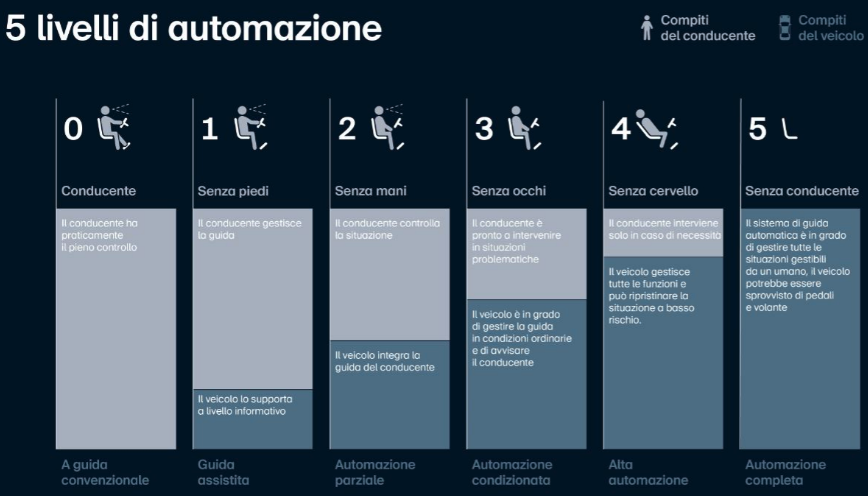
\includegraphics[width = \linewidth]{5 livelli.png}
    \centering
    \caption{Livelli di automazione definiti dalla SAE International.}
    \label{sae}
\end{figure}
\begin{enumerate}
    \setcounter{enumi}{-1}
    \item \emph{A guida convenzionale}:  Non esiste alcun tipo di automazione. Il 
    conducente è responsabile della guida.
    \item \emph{Guida assistita}: il veicolo è dotato di sistemi di assistenza alla guida 
    che consentono per esempio il controllo longitudinale (Cruise control) 
    o trasversale (mantenimento di corsia). Questi assumono il controllo 
    di alcune funzioni del veicolo, come accelerazione, frenata, parcheggio 
    e/o sterzata. Tali sistemi si alternano con il guidatore che dev'essere 
    sempre pronto ad intervenire o a riprendere in maniera autonoma il 
    controllo del veicolo.
    \item \emph{Automazione parziale}: il sistema deve assicurare il controllo della 
    direzione trasversale e longitudinale in situazioni particolari come per 
    esempio un sorpasso. Anche in questo livello è richiesta l'attenzione 
    del guidatore.
    \item \emph{Automazione condizionata}: questo livello corrisponde ad una guida 
    totalmente automatizzata. In questo caso il conducente non è tenuto 
    costantemente a sorvegliare il veicolo ma dev'essere comunque pronto 
    a riprendere la situazione sotto il proprio controllo quando il sistema 
    lo avvisa.
    \item \emph{Alta Automazione}: il sistema assume la piena conduzione del veicolo 
    in maniera del tutto automatica. Questo livello si applica su determinati 
    tratti stradali, come per esempio in autostrada in quanto meno 
    complessa. Il veicolo può disattivarsi solo se il conducente riprenderà 
    il pieno controllo causa arresto sulla corsia di emergenza. 
    \item \emph{Automazione completa}: massimo livello di automazione raggiunto 
    dal sistema. Il veicolo assume il totale controllo, a prescindere dalla 
    tipologia di strada intrapresa, pertanto non richiede la presenza 
    di alcun conducente.
\end{enumerate} 
Un sistema di guida autonoma, per poter garantire la sicurezza, può possedere 
diverse funzionalità come: Rilevamento della strada (Road Detection), 
rilevamento della corsia (Lane detection), rilevamento dei veicoli (Vehicle 
detection), rilevamento dei pedoni (Pedestrian detection), rilevamento della 
stanchezza/sonnolenza (Drowsiness detection) , prevenzione delle collisioni 
(Collision avoidance) e il rilevamento della segnaletica stradale (Traffic sign 
detection).
\subsubsection{Road detection}
Questa tecnica mira a rilevare le aree e i confini in cui un veicolo può circolare 
in maniera autonoma. Tra le tecniche più utilizzate per il rilevamento 
della strada è senz'altro quella della segmentazione. Diversi sono stati i 
lavori proposti incentrati su questa tematica. Per esempio in \cite{Up-conv-Poly} viene 
introdotto un modello, nominato Up-Conv-Poly, in cui viene combinata una 
rete FCN con una rete U-Net. Quest'ultimo è in grado di effettuare delle 
segmentazioni veloci e a un basso costo computazionale grazie alla modifica 
della distribuzione dei parametri presenti negli strati convoluzionali della 
rete. In \cite{CALTAGIRONE2019125} è stato prodotto un modello, chiamato LidCamNet, basato su 
una fully convolutional network per il rilevamento delle immagini stradali 
che fonde la segmentazione di queste con i dati provenienti da un sensore 
Ligth Detector And Range (LIDAR). Diversi sono anche stati gli studi che 
utilizzano le reti FCN che hanno portato ad ottenere le prestazioni migliori 
in questo campo. La segmentazione della strada è visto come un problema di 
classificazione binario (strada o non strada). Per citarne un'ultima, abbiamo 
il modello DEEP-DIG \cite{DEEP-DIG} che utilizza ResNet come backbone con una 
architettura FCN con multipli passaggi di upscaling utili a poter interpolare 
un'immagine. 
\begin{figure}
    \centering
    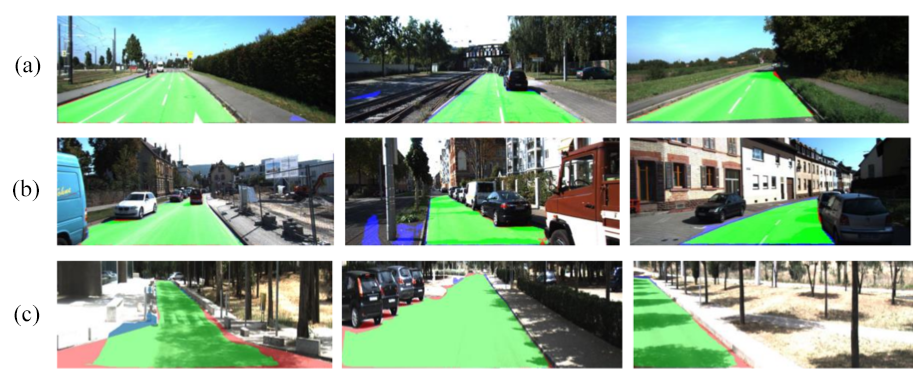
\includegraphics[width = \linewidth]{road detection.png}
    \centering
    \caption{Road Segmentation proveniente dai diversi modelli: (a) Up-Conv-Poly, (b) LidCamNet e (c) DEEP-DIG. Il colore verde indica una segmentazione True-Positive, rosso indica una rilevazione False-Negative e Blu una rilevazione False-Positive.}
    \label{road-det}
\end{figure}
La Figura (\ref{road-det}) mostra una i risultati di segmentazione stradale ottenuta 
dai tre modelli precedenti.

\subsubsection{Lane detection}
I sistemi basati sul rilevamento della corsia garantiscono il giusto posizionamento 
del veicolo nella corretta corsia, o quanto meno avvisano il guidatore, 
tramite un l'emissione di un segnale acustico, dell'imminente fuoriuscita 
da essa. Questa tecnica permette di ridurre al minimo la possibilità di 
collisione con un veicolo circolante in senso opposto. In generale, un sistema 
di lane detection esegue i seguenti passaggi \cite{lane-steps}:
\begin{enumerate}
    \item \emph{Pulizia dell'immagine (Image Cleaning)}: questa è considerata come 
    una fase di pre-elaborazione che ha diversi obiettivi. Il primo fra 
    questi è quello di rimuovere il rumore nell'acquisizione dell'immagine 
    proveniente da una camera installata frontalmente al veicolo. Successivamente, 
    tramite l'utilizzo di alcuni filtri, vengono migliorate alcune 
    feature utili per escludere gli ostacoli e ridurre la presenza delle ombre;
    \item \emph{Rilevamento delle feature (Feature Detection)}: l'obiettivo principale 
    in questa fase è quello di estrarre le feature rilevanti per poter essere 
    elaborate nella fase successiva. La segnaletica orizzontale presenta 
    diverse caratteristiche, come ad esempio la tipologia di linea (continua, 
    segmentata, doppia o singola) e il colore (bianco, giallo, blu). Particolari 
    filtri, come quello di Canny e Sobel, vengono impiegati per poter 
    rilevare queste feature. Un esempio di rilevamento sfrutta informazioni 
    quali colore e intensità. L'apprendimento di queste caratteristiche ha 
    permesso in \cite{lane-detection} una segmentazione efficiente delle linee presenti sulla 
    corsia.
    \item \emph{Adattamento del modello (Model fitting)}: in questa fase viene applicato 
    un modello geometrico sull'immagine acquisita utilizzando le 
    feature estratte precedentemente. La famiglia di modelli disponibili, 
    ad eccezione di quelli parametrici, possono essere classificati in 
    modelli semi-parametrici e non parametrici. Un esempio di modello 
    semi-parametrico può essere rappresentato dalle Splines, mentre un 
    modello non parametrico non è ancora comune;
    \item \emph{Tracciamento (Tracking)}: il sistema dev'essere in grado di supportare 
    il sistema decisionale nel selezionare la migliore linea che meglio rappresenta 
    la corsia da intraprendere. Questa tecnica è particolarmente 
    utile per poter ridurre la ROI (Region Of Interest) che corrisponde 
    alla regione di ricerca all'interno dell'immagine, riducendo a sua volta 
    il costo computazionale. Grazie ad un confronto effettuato tra i 
    vari frame, precedente e successivi, il tracciamento delle linee riduce 
    l'errore di rilevamento delle parti fuorvianti. Esistono vari sensori a 
    supporto di questa tecnica, come ad esempio i sensori IMU (Inertial 
    Measurement Unit) o il GPS che, grazie alla fusione dei loro dati, 
    contribuiscono a stimare la posizione del veicolo, e quindi a definire 
    la sua odometria, che può essere rilevante nella suddetta tecnica di 
    tracciamento.
\end{enumerate}
\begin{figure}
    \centering
    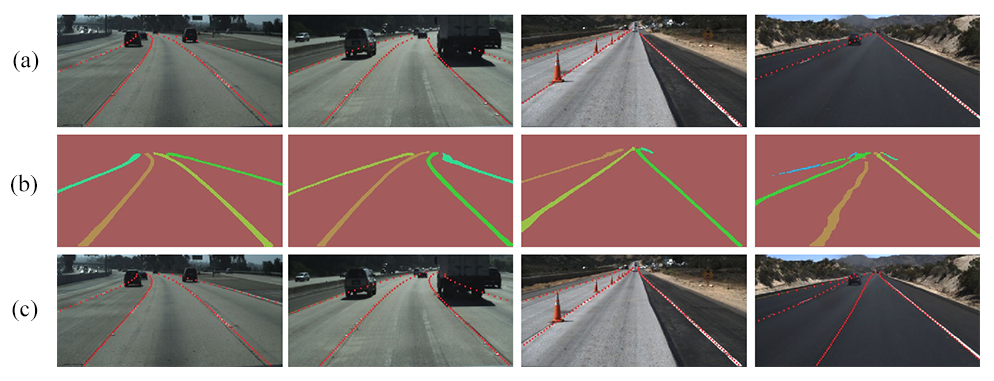
\includegraphics[width = \linewidth]{lane-detection.png}
    \centering
    \caption{Lane detection: (a) ground-truth (b) LaneNet \cite{LaneNet} output (c) model fitting.}
    \label{lane-det}
\end{figure}
In Figura (\ref{lane-det}) è possibile osservare un esempio di lane detection.

\subsubsection{Vehicle detection}
Esistono innumerevoli sfide nella computer vision per quanto riguarda il 
compito di rilevamento dei veicoli su strada. Ci sono diversi fattori mutanti 
che possono incidere sulle performance di un sistema di rilevamento, come 
per esempio le variazioni di illuminazione, forme, ombre, background etc. 
La presenza di disordine nella scena può portare all'occlusione parziale di 
un veicolo, limitandone la visibilità completa con conseguente aumento del 
rischio di incidenti. L'utilizzo delle sole telecamere comporta delle carenze 
a livello di sicurezza in quanto queste sono delle tecnologie passive, che 
non interagiscono in alcun modo con l'ambiente ed inoltre sono altamente 
influenzate dalle condizioni dell'ambiente esterno. La ricerca pertanto si 
sta spostando verso l'utilizzo di altri sensori quali telecamere con flash, 
termocamere e sistemi per la stima della profondità (es: LIDAR). Diversi 
studi hanno esaltato l'importanza del corretto posizionamento delle camere. 
Per il rilevamento e il tracciamento dei veicoli, importante risulta essere 
l'utilizzo delle simmetrie e dei bordi dei veicoli anche se negli ultimi anni si 
è preferito utilizzare altre tipologie di feature. Nello specifico, queste feature 
si riferiscono all'Istogramma dell'Orientazione del Gradiente (\emph{Histogram 
of Oriented Gradient (HOG)}) e \emph{Haar-like}, quest'ultime sono feature che 
devono il loro nome per la loro somiglianza alle wavelet Haar, entrambe molto 
diffuse in ambito di object detection e per il rilevamento dei veicoli. Un'altra 
tipologia di feature importanti sono le \emph{Scale Invariant Feature Transform 
(SIFT)}, ampiamente utilizzate per rimediare alle occlusioni parziali dei 
veicoli. Anche le Speed up Robust Features (SURF), in combinazione con i 
bordi rilevati, vengono utilizzate per poter definire delle potenziali regioni 
di interesse (ROI) in cui potrebbero esserci dei veicoli. Infine, la ricerca si è 
avvalsa di un'ultima feature largamente utilizzata nel campo della computer 
vision, si sta parlando della \emph{Principal Component Analysis (PCA)}. Allo 
stato dell'arte, l'utilizzo di tutte queste feature ha permesso di ottenere i 
risultati utili a creare dei sistemi di guida autonoma intelligenti. Un esempio 
di rilevazione e dei veicoli viene rappresentata nella Figura (\ref{vehicle-det}).
\begin{figure}
    \centering
    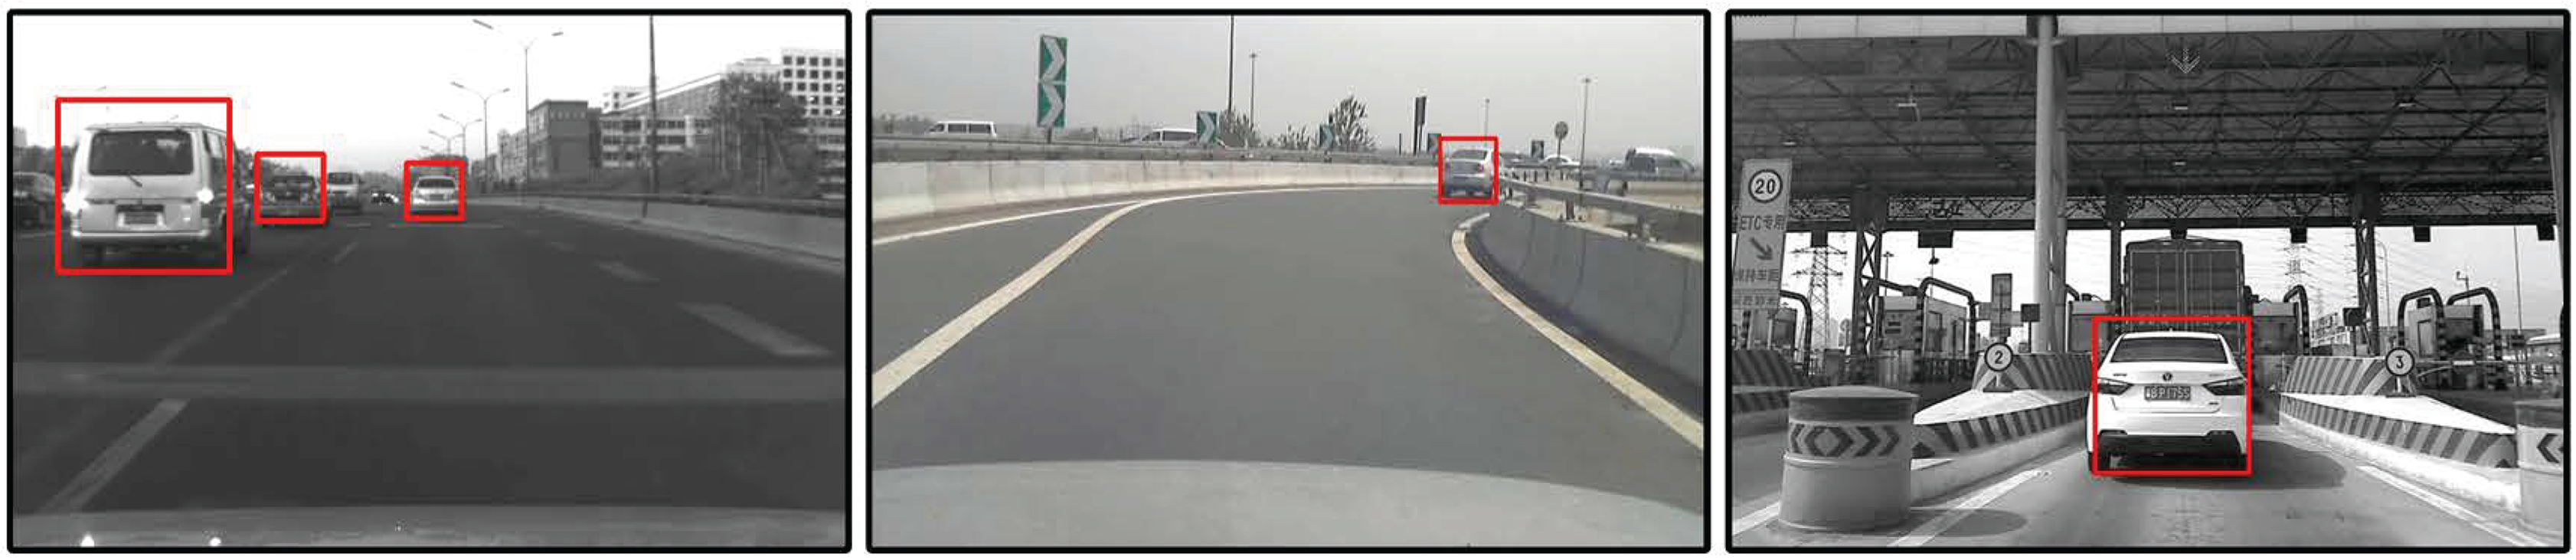
\includegraphics[width = \linewidth]{vehicle detection.png}
    \centering
    \caption{Esempio di Vehicle detection a varie distanze e illuminazioni.}
    \label{vehicle-det}
\end{figure}

\subsubsection{Pedestrian detection}
Per i veicoli a guida autonoma è importante distinguere gli oggetti dagli 
umani a causa della loro diversa importanza. Oltre che ad evitare possibili 
collisioni con i veicoli, le telecamere installate sul veicolo servono per 
rilevare uno dei principali personaggi della circolazione: il pedone. La rilevazione di 
questa classe permette una maggiore comprensione semantica della scena. I 
sistemi avanzati di assistenza alla guida (\emph{Advanced Driver Assistance Systems 
(ADAS)}) hanno lo scopo di aiutare il conducente a prendere decisioni 
e a fornire supporto durante le probabili situazioni di pericolo,  ovvero quando 
entrambi si trovano in una scena popolata da pedoni e veicoli. Esistono 
specifici sistemi ADAS per il rilevamento dei pedoni, questi prendono il 
nome di sistemi di protezione dei pedoni (\emph{Pedestrian Protection Systems 
(PPS)}). L'obiettivo di questa classe di sistemi è quello di rilevare la presenza 
di persone, sia ferme che in movimento, in una specifica regione di interesse 
(ROI) attorno al veicolo, ed eventualmente di avvisare il conducente  o eseguire 
direttamente delle azioni come una franata, o l'apertura dell'airbag, 
se vi è una possibile collisione. Le sfide principali che i sistemi PPS devono 
affrontare sono:
\begin{enumerate}
    \item \emph{Ridurre la variabilità dell'aspetto}: un pedone non può essere scambiato 
    con un oggetto se questo ha delle caratteristiche diverse, come per 
    esempio l'altezza o l'abbigliamento, o se questo assume delle pose 
    diverse;
    \item \emph{Capacità di identificazione}: i pedoni devono essere sempre identificabili 
    in un contesto disordinato, come per esempio in un'area urbana 
    dove vi sono una moltitudine di protagonisti che possono confondersi 
    con un pedone. Oltre a questo aspetto, i sistemi devono risolvere la 
    principale sfida che riguarda l'illuminazione, molte delle volte influenzata 
    dalle condizioni meteorologiche, che influenza la qualità delle 
    informazioni rilevate. Un ulteriore sfida riguarda l'identificazione dei 
    pedoni parzialmente o totalmente occlusi da elementi urbani, come i 
    veicoli parcheggiati. 
    \item \emph{Dinamicità}: il sistema deve poter identificare il pedone in scene 
    altamente dinamiche in cui sia la telecamera e il pedone sono in 
    movimento. Inoltre il sistema deve funzionare ad una distanza minima 
    di 25 metri che, corrispondenti a delle patch di pedoni di $30\times 60$ 
    pixel, utilizzando una fotocamera con lunghezza focale di $6 mm$ che 
    produrrebbe un'immagine di dimensioni $640\times 480$ pixel.
    \item \emph{Velocità}: il principale scopo di questi sistemi è quello di reagire in 
    maniera istantanea, ciò dipenderebbe da delle adeguate prestazioni e 
    da una buona robustezza da perte del sistema. Ci dev'essere il giusto 
    trade-off tra velocità e falsi allarmi o tra velocità e identificazioni 
    errate.
\end{enumerate}
Da un punto di vista pratico, per poter rilevare la presenza di uno o più 
pedoni, ogni sistema PPS effettua diverse elaborazioni \cite{pedestrian-detection}, quali:
\begin{figure}
    \centering
    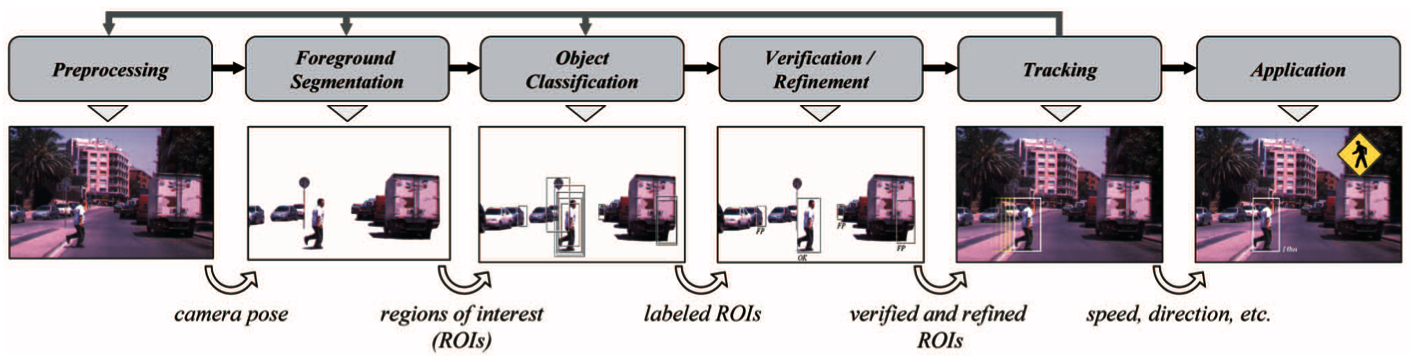
\includegraphics[width = \linewidth]{Pedestrian-detection.png}
    \centering
    \caption{Fasi di elaborazione Pedestrian detection.}
    \label{ped-det}
\end{figure}
\begin{enumerate}
    \item \emph{Pre-processing}: in questa fase vengono svolte operazioni quali calibrazione 
    della fotocamera, regolazione della gamma dinamica e correzione 
    del tempo di esposizione. Questa operazione è di fondamentale importanza 
    per il sistema PPS in quanto contrasta il cambiamento di 
    luminosità (per esempio si pensi a quando si intraprende un tunnel o 
    quando ci si trova nel bel mezzo di un temporale);
    \item \emph{Foreground segmentation}: fase in cui vengono separati il foreground 
    (possibili candidati) dal background (sfondo) per dar vita a regioni di 
    interesse (ROI) che verrano inviate al modulo di classificazione. Lo 
    scopo principale di questa fase è quello di rilevare tutti i pedoni per 
    poter ottenere dei risultati dalle fasi successive;
    \item \emph{Object classification}: dopo aver ricevuto le ROI dal modulo precedente, 
    questo modulo si occupa di verificare la presenza di un pedone al loro  
    in modo da ridurre al minimo i falsi positivi e i falsi negativi. In 
    questa fase vengono utilizzate le stesse feature impiegate nella tecnica 
    di vehicle detection. 
    \item \emph{Verification/Refinement}: diversi sistemi contengono un passaggio aggiuntivo 
    che mira alla verifica e al perfezionamento della classificazione 
    delle ROI. La fase di verifica funge da filtro per i falsi positivi, mentre 
    la fase di perfezionamento esegue delle segmentazioni precise del 
    pedone utili a fornire un'accurata distanza e supportare il successivo 
    modulo;
    \item \emph{Tracking}: la fase di tracciamento consente di seguire i pedoni dopo che 
    questi vengono rilevati nella scena. Lo scopo di questo modulo è quello 
    di evitare falsi rilevamenti nel tempo, prevedere le future posizioni, in 
    modo da generare un corretto numero di candidati utili per l'algoritmo 
    di segmentazione foreground. Un ulteriore utilizzo di questa tecnica 
    permette di rilevare ed effettuare delle stime sul comportamento di 
    ogni singolo pedone, come per esempio la previsione della direzione 
    della sua camminata;
    \item \emph{Application}: l'ultima fase di un sistema PPS riguarda il prendere 
    decisioni di alto livello, come per esempio la generazione di un avviso 
    acustico o una franata di emergenza, basandosi sulle informazioni 
    ricevute dai moduli precedenti. In questa fase vengono utilizzate 
    tecniche precedentemente citate, come la fusione dei dati provenienti 
    dai diversi sensori.
\end{enumerate}
Nella Figura (\ref{ped-det}) viene mostrato un riassunto delle precedenti fasi 
applicate ad un problema di rilevamento dei pedoni.

\subsubsection{Drowsiness detection}
La tecnologia che sta per essere introdotta riguarda i livelli 1,2, e 3 della guida 
autonoma in quanto quelli successivi richiedono parzialmente la presenza 
del conducente (livello 4) o la sua completa assenza (livello 5). La tecnica 
di \emph{Drowsiness Detection (DDT)} è la tecnica che rivela lo stato del conducente 
quando questo è alla guida. Quando il sistema rivela che il conducente risulta 
essere distratto, oppure è in uno stato di sonnolenza, può intraprendere 
automaticamente determinate azioni necessarie a scongiurare un possibile 
incidente. I metodi di drowsiness detection sono classificati in 
tre categorie \cite{drowsiness-detection}:
\begin{enumerate}
    \item \emph{Tecniche basate sulla fisiologia;}
    \item \emph{Tecniche basate sul veicolo;}
    \item \emph{Tecniche basate sul comportamento.}
\end{enumerate}
La prima categoria è in grado di rilevare la sonnolenza in base alle condizioni 
fisiche dei conducenti come la frequenza cardiaca, frequenza respiratoria, 
temperatura corporea, etc. Dal punto di vista di sicurezza, questi parametri 
sono i più affidabili in quanto fanno riferimento a ciò che sta accadendo a livello 
fisico nel conducente. Queste misure sono invasive in quanto richiedono 
sensori adatti posizionati appositamente in varie parti del corpo del conducente. 
In questo elaborato non verrà approfondita questa categoria in quanto 
non pertinente attinente allo studio proposto. La seconda categoria cerca di 
rilevare l'affaticamento del conducente in base ai dati veicolari raccolti. Tale 
tipologia di informazioni possono riguarda il cambio di corsia, la variabilità 
della velocità, l'angolo di rotazione del volante etc. L'analisi svolta su questi 
dati permette al sistema di creare dei modelli di guida e determinare se quelli 
rilevati in real-time si discostano o meno da quelli abituali. Se il sistema 
riscontrasse delle anomalie dovute a un matching sbagliato fra questi, allora 
dovrebbe prendere delle iniziative utili a salvaguardare il conducente o i 
passeggeri presenti nell'abitacolo del veicolo. Tuttavia, tale tecnica può 
essere limitata da fattori esterni quali le condizioni stradali, che possono 
provocare sbandamenti insoliti classificati come campanello d'allarme dal 
sistema, o dalle condizioni meteorologiche. Anche queste tecniche pertanto 
sono ritenute inaffidabili in questi casi. La ricerca sta puntando sull'ultima 
categoria, quella delle tecniche basate sul comportamento. Quest'ultime 
sono ritenute come misure non invasive per il rilevamento della sonnolenza. 
L'affaticamento del conducente è calcolato in base a vari fattori come il 
rapporto di chiusura degli occhi (\emph{eye closure ratio}), il battito delle palpebre 
(\emph{eye blinking}), la posizione della testa (\emph{hand position}), le espressioni facciali 
(\emph{facial expression}) e gli sbadigli (\emph{yawning}). La metrica più utilizzata per 
il rilevamento della sonnolenza si basa sull'osservazione dello stato degli 
occhi, più precisamente alla percentuale di chiusure oculari, soprannominata 
\emph{PERCLOS}. Grazie a questa ,metrica è possibile determinare se gli occhi 
sono aperti, chiusi o socchiusi. L'analisi dello sbadiglio viene effettuato 
monitorando le variazioni della forma geometrica della bocca grazie all'aiuto 
di camere o stereo-camere. Seppur ritenuta la miglior categoria a livello 
di sicurezza, questa non è esente dai problemi derivanti dai fattori esterni 
quali illuminazione e condizioni stradali. Vari sono i sitemi di classificazione 
che svolgono l'attività di drowsiness detection, fra questi abbiamo i classificatori 
\emph{Support-Vector-Machines (SVM)}, \emph{l'Hidden Markow Model (HMM)} 
e le reti neurali convoluzionali (CNN). Essendo questo uno studio incentrato 
sull'argomentazione delle reti CNN, l'algoritmo di Viola Jones \cite{viola2001rapid} 
viene molto utilizzato per il riconoscimento del viso. Le immagini di input 
vengono tutte ritagliate per assumere una dimensione pari a $48\times 48$ su 
cui verrà sottoposto un banco di 20 filtri che produrranno risultato che saranno 
tramandati al layer finale Softmax, da cui ne susseguirà la classificazione. 
Tale rete ha avuto diverse evoluzioni che hanno portato al rilevamento del 
volto anche durante i movimenti di codesto. Venne introdotto pertanto un 
rilevamento basato su tecniche 3D che includono altri due filtri oltre a quelli 
già esistenti. In Figura (\ref{drow-det}) è possibile notare un'idea generale di come un 
modello effettua una drowsiness detection.
\begin{figure}
    \centering
    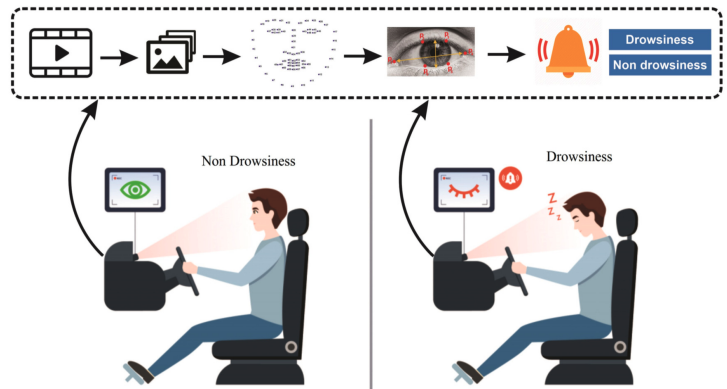
\includegraphics[width = \linewidth]{drowsiness detection.png}
    \centering
    \caption{Modello generale del sistema di Drowsiness detection.}
    \label{drow-det}
\end{figure}

\subsubsection{Collision Avoidance}
\begin{figure}
    \centering
    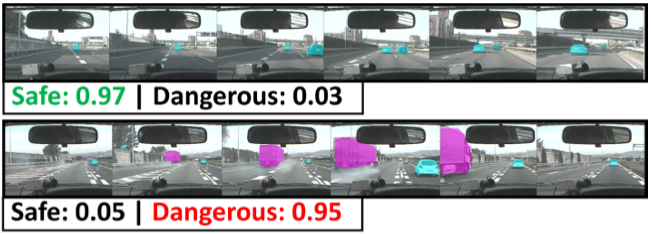
\includegraphics[width = \linewidth]{collision-avoidance.png}
    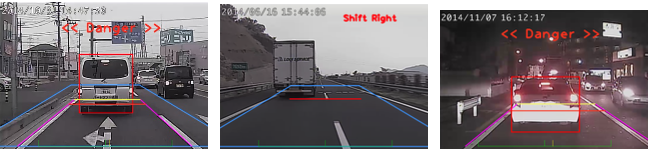
\includegraphics[width = \linewidth]{collision-avoidance 2.png}
    \centering
    \caption{Esempio di alcuni sistemi di Collision Avoidance.}
    \label{coll-avoid}
\end{figure}
Tutte le tecniche precedenti sono in grado di aumentare il livello di sicurezza 
ponendosi l'obiettivo di tracciare con accuratezza veicoli e pedoni presenti 
nell'ambiente circostante. Ciò che non è stato ancora spiegato è il chi prende 
le decisioni importanti e come queste possano trasformarsi in azioni atte a 
mettere in sicurezza le persone coinvolte. Quando un veicolo è dotato di 
guida autonoma, la responsabilità nell'intraprendere determinare azioni/decisioni 
è demandata al sistema di prevenzione delle collisioni (\emph{Collision 
Avoidance System (CAS)}). Solitamente, tutte le informazioni sull'ambiente 
circostante relative ad altri veicoli, la segnaletica orizzontale, le informazioni 
sui segnali stradali e la velocità sono disponibili in un data base centrale 
dinamico (\emph{Dynamic Data Base (DDB)}). Grazie a questo, gli algoritmi di 
controllo e pianificazione riescono a comunicare tra loro. Possiamo considerare 
il CAS come un sistema che, durante la velocità desiderata e il 
comportamento di guida desiderato, minimizza il rischio di collisioni. Per 
realizzare ciò, vengono utilizzati due approcci. Il primo viene chiamato 
il metodo del campo potenziale \cite{col-avoid} che ha il compito di trovare il punto 
minimo all'interno di una mappa del rischio e allo stesso tempo di manovrare 
il veicolo in modo appropriato. Il secondo metodo viene chiamato sistema di 
transazione statale \cite{col-avoid2}. In quest'ultimo vengono considerati tutti i possibili 
casi, condizioni e situazioni. Diversi sono stati gli studi che hanno portato 
ad effettuare stime del rischio durante la guida. Una delle principali azioni 
che è viene considerata altamente rischiosa è quella inerente al cambio corsia. 
Diversi studi \cite{risk} sono stati applicati per poter minimizzare il rischio riguardante 
questa problematica. L'utilizzo di reti profonde, nello specifico delle 
\emph{Recurrent Neural Network (RNN)}, e di opportune tecniche di segmentazione, 
hanno prodotto una serie di risultati incoraggianti che hanno contributo 
allo sviluppo di sistemi utili alla minimizzazione del rischio.  Per poter 
calcolare il livello di rischio bisogna considerare i tratti umani (stili di guida) 
del guidatore affinché venga prodotta una previsione sulle intenzioni dei 
possibili personaggi che compongono l'ambiente esterno (pedoni e veicoli). 
In Figura (\ref{coll-avoid}) è possibile notare alcuni sistemi di Collision Avoidance.

\subsubsection{Traffic Sign/Light Detection and Recognition}
Un'alta percentuale di incidenti stradali è dovuta alla scarsa attenzione verso 
la segnaletica stradale. Un sistema di guida autonoma, grazie a tecniche di 
computer vision e grazie al supporto del deep learning, può essere in grado 
di rilevare segnaletiche stradali quali strisce pedonali, incroci, semafori etc. 
Come tutte le altre tecniche, la tecnica di \emph{Traffic Sign Recognition (TSR)} e 
la tecnica di \emph{Traffic Light Recognition (TLR)} hanno il compito di avvisare 
il guidatore quando questo si trova in prossimità di un'area che richiede 
attenzione, come per esempio una curva o un incrocio. La rilevazione di 
queste aree viene fatta grazie all'utilizzo delle \emph{Region Based Convolutional 
Neural Networks (R-CNN)} \cite{RCNN-TLR}, reti neurali in grado di estrarre le regioni 
di interesse (ROI). Ogni regione estratta verrà analizzata da una rete 
convoluzionale per poter identificare gli oggetti al suo interno. In genere, 
il TSR è diviso in due categorie: Detection e Classification. La detection 
riguarda la localizzazione della segnaletica stradale nelle varie ROI, mentre la 
classificazione riguarda al determinazione del tipo di segnale che il sistema 
ha rilevato. Oltre che a riconoscere i segnali, un TSR dev'essere anche 
intelligente. Durante il percorso, se il sistema rivela più segnali ridondanti, 
questo non deve attirare la concentrazione del conducente in quanto non tutti 
i segnali hanno la stessa importanza. Quando un segnale viene rilevato più 
volte in maniera consecutiva, il sistema dovrebbe notificarlo una sola volta 
o quanto meno dovrebbe avvertire solo in caso di segnaletica importante. 
Oltre a questo aspetto, un TSR dev'essere in grado di rilevare quei segnali 
che il guidatore non ha colto, a causa di una distrazione, durante il tragitto. 
I sistemi TSR sono in grado di gestire i falsi positivi e i falsi negativi. Tutto 
questo è possibile grazie a un confronto fra frame adiacenti in cui vengono 
rilevati e tracciati i vari segnali. Se un segnale venisse erroneamente rilevato 
in un solo frame e non in quelli adiacenti, allora potrebbe trattarsi di un 
falso positivo e pertanto non c'è bisogno di notificarlo al conducente. Oltre 
alla velocità assunta dal veicolo, che potrebbe influenzare la classificazione, 
ovviamente ci dev'essere un corretto trade-off tra la velocità di rilevazione e 
il tempo di riconoscimento del segnale. Quando si confrontano i rilevatori 
di segnali, è necessario impostare alcune metriche di confronto. Come al 
solito, la misura più semplice e la più importante è il tasso dei veri positivi.
La fase di identificazione è di solito suddivisa un due sottofasi \cite{sign-rec}:
\begin{enumerate}
    \item \emph{Metodi basati sul colore;}
    \item \emph{Metodi basati sulla forma.}
\end{enumerate}
Il colore e la forma possono contraddistinguere un segnale da un altro.
Ogni metodo ha i suoi pro e i suoi contro. Se la ricerca è incentrata sul 
colore allora questa potrebbe essere influenzata da fattori esterni come 
l'illuminazione o l'aspetto del segnale (presenza di imbrattature, adesivi 
o semplice sbiadimento). Al contrario, risulta facile ricercare un range di 
colori all'interno di un'immagine. Per quanto riguarda le forme, queste 
sono invarianti all'illuminazione e al tempo mentre, d'altra parte se occluse 
rappresentano una problematica per il rilevamento. Per risolvere i problemi 
inerenti il rilevamento, viene utilizzata la tecnica di segmentazione che segue 
una fase di estrazione delle feature per poter successivamente eseguire il 
rilevamento del segnale. Lo scopo della segmentazione è quello di ottenere 
un'area approssimativa di dove dovrebbero comparire i segni stradali per 
poter quindi restringere lo spazio di ricerca nelle fasi successive. La fase 
di feature extraction ricerca maggiormente elementi appartenenti al set di 
forme geometriche come angoli, bordi, cerchi, rettangoli etc. Per questo 
scopo, una delle tecniche maggiormente utilizzate per l'estrazione delle 
feature è la trasformata di Hough o le già citate wavelet di Haar. Un 
esempio di Traffic Sign e Light recognition è riportato nella Figura (\ref{traffic sing-ligth}).
\begin{figure}
    \centering
    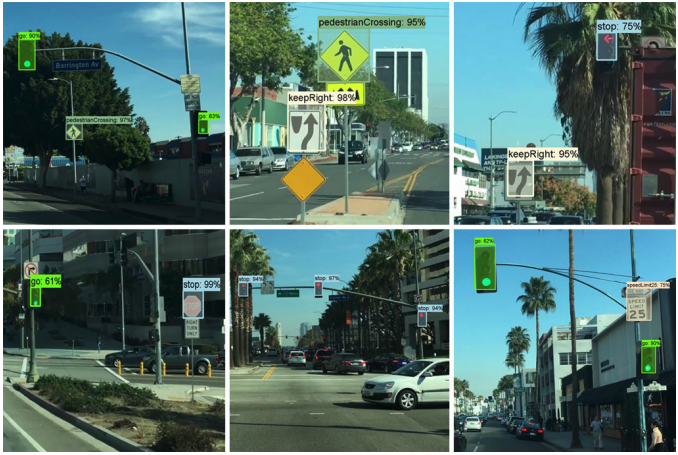
\includegraphics[width = \linewidth]{traffic sign and ligth.png}
    \centering
    \caption{Esempio di Traffic Sign/Light recognition.}
    \label{traffic sing-ligth}
\end{figure}

\section{Tecniche di compressione/ottimizzazione delle reti neurali.}
Le reti neurali sono largamente diffuse in molteplici dispositivi IoT e sistemi 
embedded. Purtroppo, alcuni modelli, a causa dell'enorme requisito 
di calcolo, energia e archiviazione, non possono essere distribuiti su tali 
dispositivi. Pertanto, negli ultimi anni, sono state proposte diverse tecniche 
di compressione in grado di implementare suddetti modelli anche su sistemi 
economici a ridotta potenzialità computazionale. Il principale requisito 
minimo, da parte di queste tecniche, riguarda il raggiungimento di un compromesso 
a basso impatto sull'accuratezza di ogni modello. Ciò che si sta 
cercando di raggiungere è quindi un metodo che sia in grado di ottimizzare 
sia le performance di un sistema, ospitante un modello deep learning, che la 
sua riduzione energetica, oltre a determinare un risparmio dello spazio di 
archiviazione. Le tre tecniche maggiormente diffuse allo stato dell'arte sono:
\begin{enumerate}
    \item {\bfseries{\emph{Pruning}}}: La tecnica di pruning ha l'obiettivo di ridurre le dimensioni 
    di un modello andando a rimuovere componenti superflui quali canali, 
    filtri, neuroni o interi livelli. La potatura può essere applicata solo in 
    maniera iterativa su un modello (\emph{Iterative Pruning}) durante il processo 
    di addestramento, oppure direttamente sul modello pre-addestrato 
    (\emph{One-shot Pruning}).
    \item {\bfseries{\emph{Knowledge Distillation}}}: tecnica in grado di trasferire la capacità 
    di generalizzazione, proveniente da un modello ingombrante chiamato 
    "\emph{Insegnante}", verso un modello più piccolo chiamato "\emph{Studente}", per 
    migliorare le prestazioni di quest'ultimo.
    \item {\bfseries{\emph{Quantization}}}: la riduzione del numero di bit necessari 
    alla memorizzazione dei pesi rappresenta una tecnica di compressione. Passare da 
    una precisione FP32 a una INT8 significherebbe ridurre di un quarto 
    la rappresentazione di un valore.
\end{enumerate}
Di seguito vengono riportate le spiegazioni più dettagliate di ciascuna.

\subsection{Quantization}
La rappresentazione dei parametri, di una rete neurale, avviene utilizzando 
un determinato numero di bit. Trovandoci in un contesto di compressione, e 
di ottimizzazione, diversi sono stati gli studi che hanno avuto l'obiettivo di 
ridurre la quantità di bit preservando l'accuratezza del modello. Allo stato 
dell'arte, tutti questi sforzi hanno dato vita allo sviluppo di una tecnica 
fondamentale: la quantizzazione. La sua popolarità è rapidamente cresciuta 
grazie agli evidenti miglioramenti delle prestazioni dei modelli. I benchmarks 
pubblicati in uno studio \cite{quantization_speed} hanno evidenziato come la quantizzazione possa 
migliorare il proprio throughput di un fattore pari a 10x. La compressione 
effettuata dalla quantizzazione si traduce in una riduzione della precisione 
Floating-Point durante le operazioni matematiche svolte all'interno della 
rete. Poiché possiamo avere numeri infinitamente precisi, ma uno spazio 
limitato in cui memorizzarli, bisogna giungere ad un compromesso tra 
precisione (il numero di decimali che si vogliono includere in un numero 
prima di arrotondarlo) e spazio (quantità di bit da utilizzare per salvare 
il numero). Secondo lo standard tecnico per i numeri a virgola mobile, 
\emph{IEEE-754} stabilisce i seguenti standard:
\begin{itemize}
    \item \emph{FP64}: conosciuto come "\emph{double-precision}" o semplicemente "\emph{double}". 
    \item \emph{FP32}: conosciuto come "\emph{single-precision}" o semplicemente "\emph{single}".
    \item \emph{FP32}: conosciuto come "\emph{half-precision}" o semplicemente "\emph{half}".
\end{itemize}
La quantizzazione ha l'obiettivo di mappare i valori aventi precisione FP32 
in valori a precisione int8. Questo vuol dire passare da una quantità di valori 
memorizzabili pari a $2^{31}$, a una quantità  corrispondente a un massimo 256 
valori, ovvero a $2^8$. La riduzione totale porta ad occupare un numero di bit 
pari a $\frac{1}{4}$ di quelli occupati dalla precisione FP32. Tale beneficio, tradotto in 
termini di performance, dovrebbe portare ad un incremento della velocità di 
inferenza per un fattore massimo pari a quattro volte. Purtroppo, quest'ultimo 
evento non sempre è verificabile. Secondo alcuni test \cite{LIANG2021370}, utilizzando 
frameworks come Google TensorFLow-Lite e NVidia TesnorRt, impostando 
un basso valore di batch-size, riescono a raggiungere un velocità massima 
di circa 2-3x. Aumentando il numero di batch-size, solamente TensorRT 
riesce ad intensificare ulteriormente la velocità di inferenza arrivando a 
3-4x. Dopo aver convertito i parametri come pesi, input e vettori intermedi, 
la maggior parte della matematica che segue viene eseguita in INT8. Una 
prima dimostrazione di tale tecnica, a precisione INT8, venne riportata 
in una ricerca \cite{37631}, nell'anno 2010. I risultati ottenuti con pesi mappati 
a una precisione INT8 hanno portato a un'accelerazione dell'inferenza 
senza avere un calo significativo dell'accuratezza. Di solito, la precisione 
utilizzata durante l'allenamento di una rete è la FP32. Per molte reti, una 
rappresentazione FP32 risulta essere una precisione maggiore del necessario.
La riduzione della precisione, oltre a comprimere un modello, mira alla riduzione della 
quantità energetica impiegata dovuta alla ridotta larghezza 
di banda (bandwidth) utilizzata. Esistono tre tiplogie di quantizzazione:
\begin{enumerate}
    \item \emph{Dynamic Quantization}: viene eseguita a runtime su un modello pre-addestrato. 
    L'operazione si basa nel moltiplicare i valori di input 
    per un fattore di scala variabile da cui seguirà un arrotondamento al 
    numero intero più vicino. Successivamente memorizza il risultato ottenuto. 
    I pesi vengono quantizzati immediatamente mentre le attivazioni 
    vengono quantizzate dinamicamente durante l'inferenza. Purtroppo, 
    questo tipo di metodo non è altamente utilizzato in quanto risulta 
    essere la meno performante, ottenendo delle performance negative.
    \item \emph{Static Quantization}: viene eseguita dopo la fase di allenamento su un 
    modello pre-addestrato. La differenza con la tecnica dinamica riguarda 
    il pre-calcolo delle scale e i punti zero di ogni tensore di attivazione 
    servendosi di dati non strutturati. Oltre ad essere più precisa rispetto 
    alla tecnica dinamica, ottiene delle migliori performance per quanto 
    riguarda l''inferenza della rete.
    \item \emph{Quantization-Aware-Training (QAT)}: risulta essere la tecnica di quantizzazione 
    più accurata. Viene svolta durante il processo di allenamento 
    ma al contempo ne rallenta i tempi di formazione del modello. 
    L'idea di tale tecnica è quella di tenere conto della perdita che si ha 
    nel processo di allenamento durante la conversione del modello.
\end{enumerate}


\subsection{Pruning}
Diversi modelli soffrono di una problematica comune: la numerosità 
dei parametri. I parametri che appaiono insignificanti, a livello di accuratezza, 
costituiscono un punto dolente dal punto di vista dell'occupazione della memoria e della 
velocità di inferenza. Prendendo in considerazione i pesi di 
ogni modello, che a loro volta costituiscono il maggior numero di parametri, 
questi possono essere considerati rilevanti quando hanno un valore divergente 
da zero. Uno o più pesi quindi sono da considerarsi irrilevanti quando 
assumono un valore prossimo allo zero. La sovrabbondanza di quest'ultimi 
impatta drasticamente sulle performance del modello. Allo stato dell'arte 
sono stati proposti diversi approcci \cite{salama2019pruning} utili a mitigare la sparsità di tali 
valori. Tutti questi sforzi hanno dato vita alla tecnica di \emph{Pruning} (Potatura).  
Esistono diverse tecniche di pruning, ovvero:
\begin{figure}
    \centering
    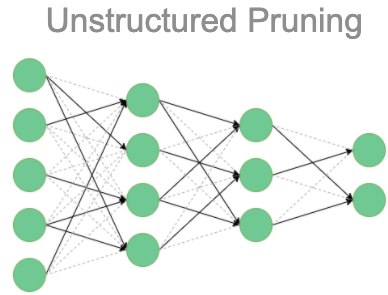
\includegraphics[width = 0.6\linewidth]{unstructured pruning.png}
    \centering
    \caption{Esempio di rete fully connected potata con la tecnica unstructured.}
    \label{unstruct-prun}
\end{figure}

\begin{figure}
    \centering
    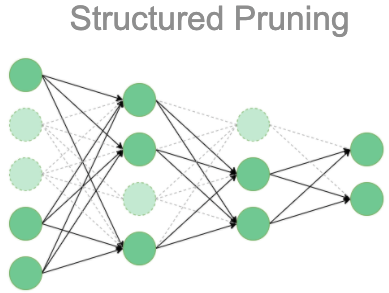
\includegraphics[width = 0.6\linewidth]{structured pruning.png}
    \centering
    \caption{Esempio di rete fully connected potata con la tecnica structured.}
    \label{struct-prun}
\end{figure}

\begin{enumerate}
    \item {\bfseries{\emph{Pruning non-strutturato (Unstructured)}}}: applicato per attività 
    di "\emph{weight pruning}"\cite{NIPS1989_6c9882bb} \cite{NIPS1992_303ed4c6}. Lo scopo di questa tecnica è quello di 
    rimuovere interi pesi introducendo quasi sempre un'elevata sparsità 
    nel modello richiedendo al contempo l'utilizzo di hardware e software 
    dedicati. La potatura dei pesi comporterebbe l'eliminazione di alcuni 
    collegamenti tra i vari neuroni, ma non la loro disattivazione (Fig. 
    \ref{unstruct-prun})
    \item {\bfseries{\emph{Pruning strutturato (Structured)}}}: tecnica che va a rimuovere interi 
    filtri (canali), o neuroni, al posto di singoli pesi, alleviando il problema 
    della sparsità. A questo proposito, \cite{li2017pruning} propose una "\emph{channel-wise 
    pruning}" in accordo con la norma \emph{L1} del filtro corrispondente. La 
    potatura strutturata in genere porta a prestazioni di runtime migliori 
    rispetto alla potatura non strutturata in quanto le operazioni vengono 
    eseguite su matrici dense. Contrariamente, questa tecnica impatta 
    pesantemente sull'accuratezza del modello. Questa tecnica, in un 
    contesto di reti fully connected, va a disattivare tutte le connessioni 
    di determinati nodi rendendoli obsoleti (Fig. \ref{struct-prun}).
    \item {\bfseries{\emph{Pruning non strutturato globale (Global Unstructured)}}}: rispetto 
    alla tecnica non strutturata, la globale applica una potatura su 
    tutti i parametri specificati in tutti i filtri appartenenti ad ogni layer 
    in maniera parallela. È importante notare che la tecnica globale di 
    unstructured pruning consente di potare i layers meno utili (entropia 
    inferiore) rispetto a quelli più utili (entropia più elevata).
\end{enumerate}

\begin{figure}
    \centering
    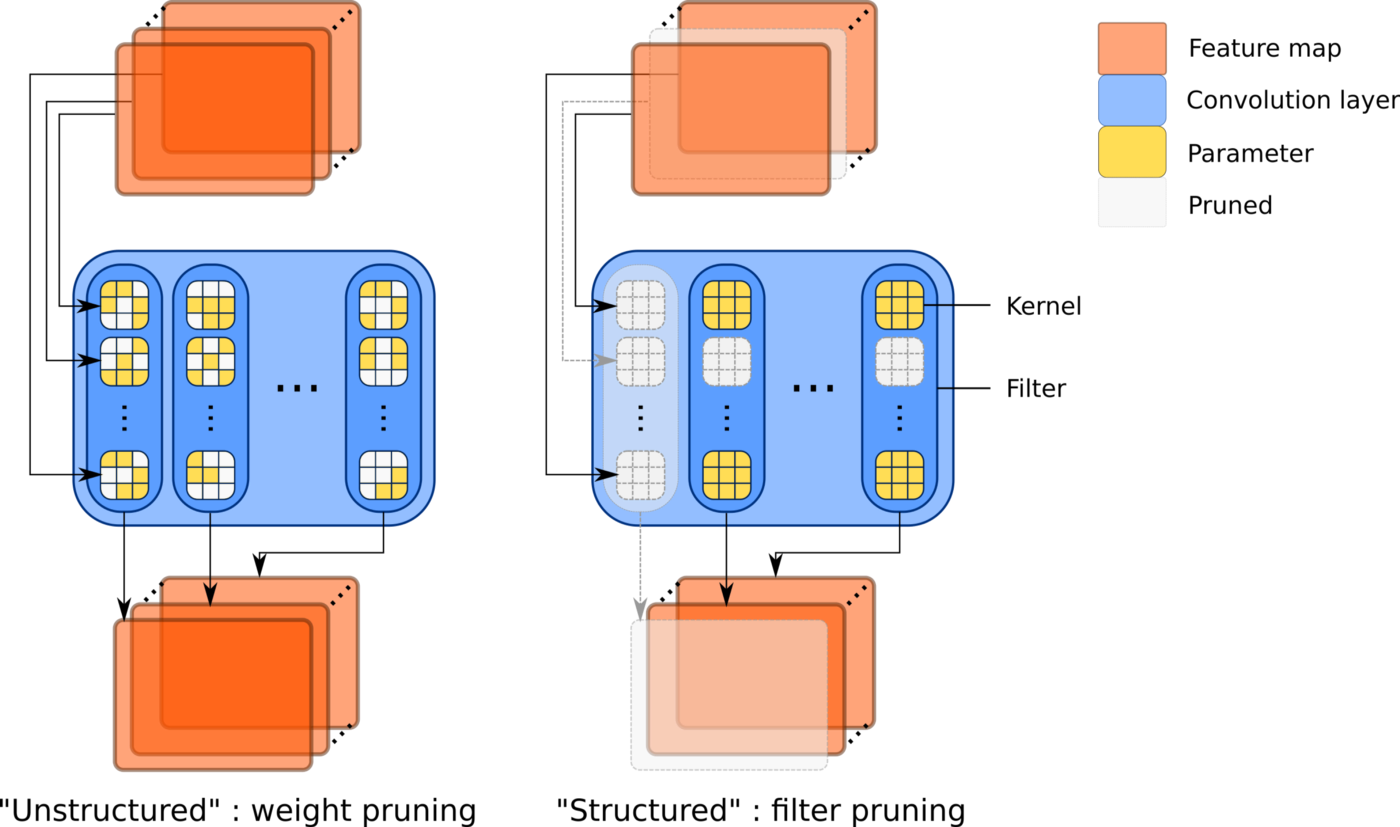
\includegraphics[width = \linewidth]{structured and unstructured pruning.png}
    \centering
    \caption{Differenza tra Ustructured Pruning (sinistra) e Structured Pruning (destra) su ogni filtro e feature maps nei vari layers.}
    \label{filter-pruning}
\end{figure}

La domanda sorge spontanea. Quali tipi di parametri dovranno essere 
sottoposti a potatura? Un criterio abbastanza intuitivo ed efficiente riguarda 
la potatura dei pesi il cui valore assoluto (o magnitudo) è il più piccolo. 
Sebbene questo criterio sembri banale da implementare in un dominio di 
unstructured pruning, ci si può chiedere come adattarlo ad una structured 
pruning. In quest'ultimo caso, per determinare l'importanza di un valore, 
queste tecniche utilizzano le norme L1 (Geometria dei Taxi/Distanza di 
Manhattan) e L2 (Distanza Euclidea) come regolarizzatori. Nello specifico, 
la relativa importanza di un filtro, in ogni layer, viene misurata calcolando 
la somma dei valori assoluti dei suoi pesi, cioè la sua norma (L1 o L2). 
Successivamente, questi filtri vengono ordinati in base al precedente risultato 
e potati se assumo il valore più basso. La potatura di un filtro porta 
all'azzeramento di un intera feature maps. Rispetto ad una unstructured 
pruning, dove l'azzeramento di un parametro influenzerebbe minimamente 
il kernel nel successivo layer, in un contesto structured ciò comporterebbe 
l'eliminazione del kernel, corrispondente a tale feature maps, presente nel 
layer successivo (Fig. \ref{filter-pruning}). Attualmente la ricerca è suddivisa su due linee di 
pensiero. Da una parte si pensa che la tecnica di pruning porti effettivamente 
al miglioramento delle performance di un modello, dovuto dalla riduzione 
delle sue dimensioni  \cite{han2015learning} e al conseguente risparmio energetico \cite{yang2017designing}, dall'altra 
parte invece si afferma tutto il contrario \cite{cheng2020survey}. Un recente studio, intitolato 
"\emph{The lottery ticket hypothesis}" \cite{frankle2019lottery} ha intensificato l'interesse per le tecniche 
di potatura. Tale studio sostiene la seguente tesi: 
\begin{displayquote}
    \emph{"Una rete neurale densa contiene una sottorete più piccola che 
    può raggiungere la stessa accuratezza, dell'intera rete originale, 
    dopo essere stata sottoposta a un processo di addestramento 
    individuale per lo stesso numero di epoche."}
\end{displayquote}
Questa ideologia ha portato gli autori ad attuare la tecnica di pruning 
iterativa utile a ricavare dei modelli più piccoli (i cosiddetti "\emph{winning 
tickets}") che hanno pienamente confermato la veridicità della propria tesi.
Sempre secondo \cite{frankle2019lottery}, l'introduzione di una crescente percentuale di sparsità 
all'interno di un modello mai ri-addestrato, porterà codesto ad avere un lento 
apprendimento in fase di training oltre che a un decremento dell'accuratezza.

\subsection{Knowledge Distillation}
I modelli profondi hanno avuto considerevoli successi, tuttavia l'elevata richiesta 
computazionale e l'aumento della richiesta di archiviazione, rendono 
difficile la loro implementazione in applicazioni real-time, specialmente su 
dispositivi con risorse limitate come la videosorveglianza e la guida autonoma. 
Questa grande limitazione ha aperto le porte allo sviluppo di una 
nuova tecnica di compressione/ottimizzazione delle reti neurali chiamata 
\emph{Knowledge Distillation} (Conoscenza distillata). Tale tecnica risulta utile 
per migliorare l'accuratezza di una piccola rete, chiamata "Studente", trasferendo 
la conoscenza distillata prodotta da una (o anche molteplici) rete 
più grande chiamata "Insegnante" (Fig. \ref{KD_simple}).
\begin{figure}
    \centering
    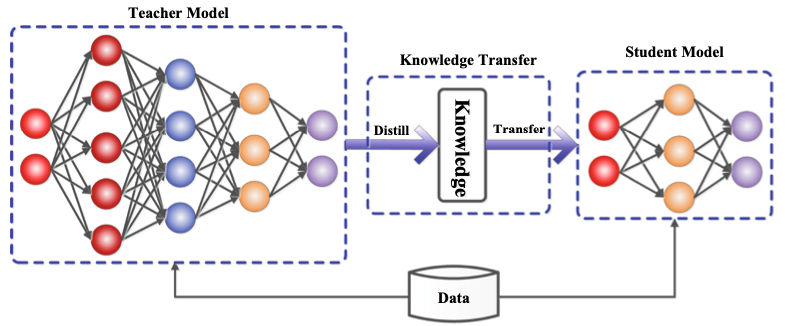
\includegraphics[width = \linewidth]{KD simple.png}
    \centering
    \caption{Il quadro generico insegnante-studente per la distillazione della conoscenza}
    \label{KD_simple}
\end{figure}
È bene non confondere tale 
argomento con il concetto di "Transfer Learning". L'obiettivo del Transfer 
Learning è quello di trasferire i pesi da un modello pre-addestrato verso 
un nuovo modello, entrambi esattamente con la stessa architettura di rete. 
Questo vuol dire che la nuova rete è profonda e complessa quanto la rete pre-addestrata.
L'obiettivo della Knowledge distillation è nettamente differente.
In \cite{hinton2015distilling} gli autori hanno mostrato che le conoscenze su "come generalizzare", 
possono essere trasferite da un insegnante verso uno studente mediante i 
cosiddetti "\emph{soft targets}". Utilizzando i logits del modello insegnante, che 
altro non sono che distribuzioni di probabilità sulle classi, si può attuare 
il principio cardine su cui è basata la knowledge distillation (o \emph{Vanilla 
Knowledge Distillation}). Il modello studente verrà allenato utilizzando i 
suddetti logits come conoscenza distillata, con lo scopo di ridurre al minimo 
l'entropia incrociata tra i logits dell'insegnante e i propri logits prodotti. 
Prima di introdurre il concetto principale, bisogna ricordare come una 
funzione Softmax (o funzione di attivazione) trasformi i numeri (logits) in 
delle probabilità che se sommate producono un valore sempre uguale a 1.  
Lo scopo di tale funzione quindi è quello di generare un range di valori, 
compresi tra 0 e 1, in cui il valore più grande rappresenterà la probabilità 
della classe target. Per calcolare la probabilità individuale di una classe 
(Softmax), viene utilizzata la seguente formula:
\begin{equation}\label{softmax_normal}
    q_j = \frac{exp(z_j)}{\sum_{k=1}^K exp(z_k)}
\end{equation}
dove:
\begin{itemize}
    \item $q_j$: probabilità della classe $j$-esima;
    \item $z_J$ logit corrispondente alla classe $j$-esima;
    \item $\sum_{k=1}^K exp(z_k)$: termine di normalizzazione;
    \item $K$: numero di classi.
\end{itemize}
La formula (\ref{softmax_normal}) calcola il rapporto tra l'esponenziale del valore di input 
dato e la sommatoria dei valori esponenziali di tutti i valori presenti negli 
inputs. Le probabilità risultati vengono chiamate "\emph{hard-targets}" (o hard 
labels). Per allenare il modello studente, bisogna modificare la suddetta 
formula (Eq. \ref{softmax_normal}) applicata dalla funzione Softmax nella seguente formula:
\begin{equation}
    q_j = \frac{e^{z_j/T}}{\sum_{k=1}^K e^{z_k/T}}
\end{equation}
dove:
\begin{itemize}
    \item $T>1$: indica un parametro chiamato \emph{Temperatura} \cite{marino2021compact}.
\end{itemize}
Le probabilità risultanti da questa softmax modificata, prenderanno il nome 
di "\emph{soft-targets}" (o soft-labels). Arrivati a questo punto, c'è da porsi la 
seguente domanda: Qual'è il significato delle soft-targets? Per comprendere 
questo concetto, guardiamo le figure X e Y.
\begin{figure}[]
    \begin{minipage}[t]{.45\textwidth}
        \centering
        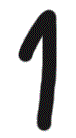
\includegraphics[width=0.5\textwidth]{number1.png}
    \end{minipage}
    \hfill
    \begin{minipage}[t]{.45\textwidth}
        \centering
        \includegraphics[width= 0.5\textwidth]{number7.png}
    \end{minipage}  
    \caption{Numeri 1 e 7.}
    \label{numbers_Mnist}
\end{figure}
Entrambi sono due numeri, l'1 
e il 7. Ciò che viene immediatamente notata è la somiglianza tra questi due 
numeri, ma nonostante ciò sappiamo distinguerli. Avere una buona capacità 
di distinzione di tali numeri vuol dire avere una buona "\emph{generalizzazione}". 
\begin{displayquote}
    \emph{"La generalizzazione è la capacità di ottenere delle predizioni 
    attendibili su nuovi dati mai utilizzati in fase di allenamento 
    da parte di un modello."}
\end{displayquote}
Quando un modello riuscirà ad intuire una somiglianza tra i due numeri, 
e allo stesso tempo a distinguerli, vuol dire che ha una buona capacità di 
generalizzazione. La temperatura è utile a controllare l'importanza di ogni 
probabilità prodotta utile a determinare il grado di generalizzazione. Dai 
risultati restituiti dal modello (Fig. \ref{7_1}), si può osservare che la probabilità 
di predire il numero 7 si "ammorbidisce" all'aumentare della temperatura T.
\begin{figure}
    \centering
    \includegraphics[width = \linewidth]{graph_numbers.png}
    \centering
    \caption{Previsione di probabilità per la cifra del numero '7' a temperature variabili.}
    \label{7_1}
\end{figure}
Seguendo la linea verde, indicante la temperatura T=7, capiremmo già da 
subito che, con un'alta confidenza, il numero target predetto dal modello è 7 
ma, allo stesso tempo, notiamo che la probabilità dei numeri 1 e 9 è più alta 
rispetto a 6. Perché accade ciò? Semplicemente perchè tra il numero 7 e i 
due numeri 1 e 9, il modello percepisce un livello di somiglianza. Prendendo 
ora in considerazione le linee blu e arancione, aventi corrispettivamente 
temperatura T=1 e T=3, si può osservare che il modello prevede giustamente 
il numero 7, ma contemporaneamente non è più in grado di distinguere se il 
numero 7 è più vicino a 1 o a 6, in quanto entrambi questi numeri hanno 
probabilità molto vicine allo zero. L'unica differenza tra un umano e un 
modello è che quest'ultimo sa quantificare precisamente, attraverso l'utilizzo 
della temperatura, quanto il numero 7 sembri più vicino a 1. Questo concetto 
è diffuso sotto il nome di "\emph{Dark Knowledge}" (Conoscenza Oscura). Un 
modello a bassa temperatura, o verosimilmente i modelli a temperatura 
T=1, sono molto bravi ad effettuare previsioni difficili ma allo stesso tempo 
perdono questo concetto di conoscenza oscura. Lo scopo della Knowledge 
distillation punta a trasmettere questa conoscenza oscura da un insegnante 
ben addestrato e un modello studente più leggero. Per allenare lo studente 
sia con le soft-targets che con le hard-targets, gli autori hanno utilizzato la 
somma ponderata di due perdite. La prima perdita ($L_{soft}$) è quella ricavata 
dal calcolo dell'entropia incrociata (cross-entropy loss) tra le previsioni del 
modello studente e le label corrette fornite dal ground-truth. La seconda 
funzione di perdita ($L_{hard}$) invece si basa sul calcolo di un'entropia incrociata 
tra le soft-targets prodotte da entrambi i modelli, studente e insegnante, 
alla stessa quantità di temperatura. Matematicamente parlando, denotiamo 
corrispettivamente con $v_j$ e $z_j$ i logits di insegnante e studente. Dopo esserci 
calcolati le probabilità soft-targets $q_j$ e $p_j$ derivanti dalla softmax dello 
studente e dell'insegnante, ad una stessa temperatura T, possiamo definire 
la seconda funzione di perdita, ovvero la seconda entropia incrociata, con la 
seguente formula:
\begin{equation}\label{cross_entropy_loss}
    C(z,v) = -\sum_jp_j \log{q_j}
\end{equation}
Il gradiente derivante dal calcolo della derivata $dC/dz_J$ sull'entropia incrociata 
(\ref{cross_entropy_loss}), si ottiene con la seguente formula:
\begin{equation}\label{cross_entropy_soft}
    \frac{dC}{dz_j}=\frac{1}{T}(q_j-p_j)=\frac{1}{T}\left(\frac{e^{z_j/T}}{\sum_{k=1}^K e^{z_k/T}}-\frac{e^{v_j/T}}{\sum_{k=1}^K e^{v_k/T}}\right)
\end{equation}
La Formula (\ref{cross_entropy_soft}) permette di minimizzare l'entropia incrociata (\ref{cross_entropy_loss}) 
e a migliorare le performance dello studente sfruttando la capacità di 
generalizzazione dell'insegnante. La perdita totale del modello studente è 
data dalla somma tra la prima e la seconda funzione di perdita. ovvero 
dalla seguente formula:
\begin{equation}
    L= L_{hard}+T^2L_{soft}
\end{equation}
Poichè i magnitudi dei gradienti prodotti dai soft-targets scalano a $1/T^2$, 
è importante moltiplicare la seconda funzione di perdita per $T^2$. A livello 
grafico, la singola generazione delle due perdite è riportata nella Figura 
(\ref{l_hard_soft}). Da come possiamo vedere, la funzione di perdita $L_{soft}$ è generata 
nel blocco "Distillation", mentre la funzione di perdita $L_{hard}$ dello studente 
è generata nella parte in basso dell'immagine.
\begin{figure}
    \centering
    \includegraphics[width = \linewidth]{KD_losses.png}
    \centering
    \caption{Generazione entropie incrociate $L_{soft}$ (in alto) e $L_{hard}$ (in basso).}
    \label{l_hard_soft}
\end{figure}